\chapter{\label{app:1-proj1}Chapter \ref{ch:proj1_LS} appendix}


\section{Experimental Results under $k$-bandlimited noise}
\label{app:Experiments_Bandlimited}
In this section we provide results on synthetic datasets under $k$-bandlimtied noise.

\begin{figure*}%
    \centering
    \begin{subfigure}{0.3\columnwidth}
    \resizebox{\width}{0.62\columnwidth}{
    \includegraphics[width=\columnwidth]{figures/proj1/plots/GLR_threshold/ER_bl.png}}
    \caption{Erdős–Rényi ($\tau_{GLR\_bl}$)}
    \label{tau_GLR_bl_er}
    \end{subfigure}
    \hfill
    \begin{subfigure}{0.3\columnwidth}
    \resizebox{\width}{0.62\columnwidth}{
    \includegraphics[width=\columnwidth]{figures/proj1/plots/GLR_threshold/BA_bl.png}}
    \caption{Barabási-Albert ($\tau_{GLR\_bl}$)}%
    \label{tau_GLR_bl_BA}%
    \end{subfigure}
    \hfill%
    \begin{subfigure}{0.3\columnwidth}
    
    \resizebox{\width}{0.62\columnwidth}{
    \includegraphics[width=\columnwidth]{figures/proj1/plots/GLR_threshold/SBM_bl.png}}
    \caption{SBM ($\tau_{GLR\_bl}$)}%
    \label{tau_GLR_bl_SBM}%
    \end{subfigure}%
    \caption{$\tau_{GLR\_bl}$ for different random graph models (\#vertices = colour, bandwidth = $\frac{\text{\# vertices}}{10}$)}
\label{GLR_Threshold_plots_bl}
\end{figure*}


%ER MSEs
\begin{figure*}%
    \centering
    \begin{subfigure}{0.3\columnwidth}
    \resizebox{\width}{0.62\columnwidth}{
    \includegraphics[width=\columnwidth]{figures/proj1/LS_MSE_bl_old/ER_0pt8_500_bandwidth_50_SNRdbs_-10.0_samps_100_MSE_LS.png}}
    \caption{Bandlimited noise, SNR = $10^{-1}$}
    \label{bandlimited_MSE_subfiga}
    \end{subfigure}\hfill
    \begin{subfigure}{0.3\columnwidth}
    \resizebox{\width}{0.62\columnwidth}{
    \includegraphics[width=\columnwidth]{figures/proj1/plots/LS_MSE/ER_0pt8_500_bandwidth_50_SNRdbs_0.0_samps_100_bl_MSE_LS.png}}
    \caption{Bandlimited noise, SNR = $1$}%
    \label{bandlimited_MSE_subfigb}%
    \end{subfigure}\hfill%
    \begin{subfigure}{0.3\columnwidth}
    \resizebox{\width}{0.62\columnwidth}{
    \includegraphics[width=\columnwidth]{figures/proj1/LS_MSE_bl_old/ER_0pt8_500_bandwidth_50_SNRdbs_100.0_samps_100_MSE_LS.png}}
    \caption{Bandlimited noise, SNR = $10^{10}$}%
    \label{bandlimited_MSE_subfigc}%
    \end{subfigure}%
    \caption{Average MSE under LS on ER Graphs (\#vertices=500, bandwidth = 50) }
\label{LS_ER_MSE_fig_bl}
\end{figure*}


\begin{figure*}%
    \centering
    \begin{subfigure}{0.3\columnwidth}
    \resizebox{\width}{0.62\columnwidth}{
    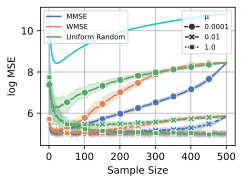
\includegraphics[width=\columnwidth]{figures/proj1/plots/GLR_MSE/ER_0pt8_500_bandwidth_50_SNRdbs_-20.0_samps_500_mus_0.0001_0.01_1_bl_noise.png}}
    \caption{Bandlimited noise, SNR = $10^{-2}$}
    \label{bandlimited_GLR_MSE_subfiga}
    \end{subfigure}\hfill
    \begin{subfigure}{0.3\columnwidth}
    \resizebox{\width}{0.62\columnwidth}{
    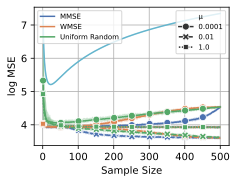
\includegraphics[width=\columnwidth]{figures/proj1/plots/GLR_MSE/ER_0pt8_500_bandwidth_50_SNRdbs_-3.01_samps_500_mus_0.0001_0.01_1_bl_noise.png}}
    \caption{Bandlimited noise, SNR = $\frac{1}{2}$}%
    \label{bandlimited_GLR_MSE_subfigb}%
    \end{subfigure}\hfill%
    \begin{subfigure}{0.3\columnwidth}
    \resizebox{\width}{0.62\columnwidth}{
    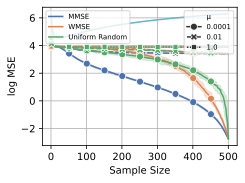
\includegraphics[width=\columnwidth]{figures/proj1/plots/GLR_MSE/ER_0pt8_500_bandwidth_50_SNRdbs_100.0_samps_500_mus_0.0001_0.01_1_bl_noise.png}}
    \caption{Bandlimited noise, SNR = $10^{10}$}%
    \label{bandlimited_GLR_MSE_subfigc}%
    \end{subfigure}%
    \caption{Average MSE under GLR on ER Graphs (\#vertices=500, bandwidth = 50), line without markers is an upper bound}
\label{GLR_ER_MSE_fig_bl}
%\label{bandlimited_GLR_ER_MSE_fig}
\end{figure*}

\subsection{\texorpdfstring{$\tau$ and $\tau_{GLR}$ plots}{\texttau and \texttau\_GLR plots}}

\subsubsection{LS}
We do not provide a plot as in this case, as our theoretical results provide the magnitude of $\tau$: by Corollary \ref {corr:LS_bandlimited_noise_sample_only_k}, $\tau(\set{S},v) = 1$ for $|\set{S}| \leq k$ under sequential noiseless-optimal sampling. Corollary \ref{corr:LS_bandlimited_noise_sample_only_k} overall says something stronger, i.e. we can always reduce MSE by reducing sample size if $\text{SNR} < 1$ at any sample size.

\subsubsection{GLR}
Our purpose in showing bandlimited variants is to show that reducing sample size can reduce MSE even under bandlimited noise. Figs. \ref{tau_GLR_bl_er}- \ref{tau_GLR_bl_SBM} show the same overall trend as Figs. \ref{tau_GLR_er}-\ref{tau_GLR_SBM}, i.e. $\tau_{GLR\_bl}$ can be positive for ER, {\color{black} BA} and SBM graphs, giving evidence to our claim. \iffalse Fig. \ref{tau_GLR_bl_BA} is entirely negative, and so entirely uninformative, i.e. it does not prove whether reducing sample size can or cannot reduce MSE under bandlimited noise for BA graphs, at least based on our theoretical results.\fi As with the full-band case, Fig. \ref{tau_GLR_bl_er} validates our asymptotic result for ER graphs (Proposition \ref{propn:GLR_big_N_bl}).

\subsection{MSE plots}
The MSE plots demonstrate the validity of our theoretical results linking MSE and sample size.

\subsubsection{LS}
Figs. \ref{bandlimited_MSE_subfiga}-\ref{bandlimited_MSE_subfigc} show how MSE behaves as sample size increases. Fig. \ref{bandlimited_MSE_subfiga} shows that under high noise, MSE increases with sample size when sample size is no larger than bandwidth, and is constant beyond that. Fig. \ref{bandlimited_MSE_subfigb} shows at an SNR of $\tau_{LS\_bl} = 1$, MSE is constant with sample size. Finally, Fig. \ref{bandlimited_MSE_subfigc} shows that in the almost noiseless case MSE decreases with sample size. Fig. \ref{bandlimited_MSE_subfiga} demonstrates Corollary \ref{corr:LS_bandlimited_noise_big_variance} by showing that for $\textrm{SNR} < \tau_{LS\_bl}=1$ the MSE is increasing with sample size. In all cases, MSE remains unchanged for sample sizes exceeding the bandlimit $k$, demonstrating Corollary \ref{corr:LS_bandlimited_noise_sample_only_k}.

\subsubsection{GLR}
Our observations about Figs. \ref{GLR_MSE_subfiga}-\ref{GLR_MSE_subfigc}  and Theorem \ref{thm:main_GLR_exist} also apply to Figs. \ref{bandlimited_GLR_MSE_subfiga}-\ref{bandlimited_GLR_MSE_subfigc} and Theorem \ref{thm:main_GLR_bl}; specifically, for sufficiently small $\mu$ and SNR, MSE is minimised at sample sizes well below $N$ under bandlimited noise and $\tau_{GLR\_bl}$ is a lower bound for $\tau(\set{N},\set{S}^{c})$ rather than an exact characterisation.

\subsection{Checking Conditions}
As in the full-band case, our theorems on GLR rely on conditions around graph invariants.  We sample graphs from each random graph model to empirically show the probability the conditions of Theorem \ref{thm:main_GLR_bl} are met at a sample size of $m_{opt}$ for some $\mu > 0$:
\vspace{-0.2cm}
\begin{table}[h!]
\caption{Probability theorem conditions are met}
    \begin{center}
        \begin{tabular}{|l|c|c|c|}
     \hline
       & \textbf{ER} & \textbf{SBM} & \textbf{BA} \\ 
     \hline
     Theorem \ref{thm:main_GLR_bl} conditions met & 100\% & 100\% & 99.4\% \\ \hline
        \end{tabular}
    \end{center}
    \label{tbl:empirical_probabilities_conditions_bl}
\end{table}
\vspace{-0.2cm}

As with full-band noise, Proposition \ref{propn:GLR_big_N_bl} shows the conditions in Theorem \ref{thm:main_GLR_bl} hold w.h.p. for ER graphs as $N \to \infty$, and Table \ref{tbl:empirical_probabilities_conditions_bl} shows empirically that the conditions hold under $k$-bandlimited noise noise (Theorem \ref{thm:main_GLR_exist}) for all ER and SBM graphs tested with $500$ vertices, and most BA graphs tested.

\section{Asymptotics}
\label{app:Asymptotics}


\section{Bias-Variance Decomposition}
\label{app:bias-variance}
We present a proof of the Bias-Variance decomposition we use. We assume that $\vect{x}$ and $\vect{\epsilon}$ are independent. Let $\hat{\vect{x}}$ be any reconstruction of the signal $\vect{x}$, then
\begin{align}
    \textrm{MSE}_{\set{S}} &= \expect[\vect{x}]{\expect[\vect{\epsilon}]{\sqnormvec{\vect{x} - \hat{\vect{x}}}}}\\
    &= \expect[\vect{x}]{\expect[\vect{\epsilon}]{\sqnormvec{\vect{x} - \expect[\vect{\epsilon}]{\hat{\vect{x}}} + \expect[\vect{\epsilon}]{\hat{\vect{x}}} - \hat{\vect{x}}}}}\\
    &= \expect[\vect{x}]{2 {\expect[\vect{\epsilon}]{ {\left(\vect{x} - \expect[\vect{\epsilon}]{\hat{\vect{x}}} \right)^{T}} {\left(\expect[\vect{\epsilon}]{\hat{\vect{x}}} - \hat{\vect{x}}\right) }}} } \label{eq:bias_variance_decomp:cross_terms} \\
    &+ \expect[\vect{x}]{{\sqnormvec{\vect{x} - \expect[\vect{\epsilon}]{\hat{\vect{x}}}}} + {\expect[\vect{\epsilon}]{\sqnormvec{ \expect[\vect{\epsilon}]{\hat{\vect{x}}} - \hat{\vect{x}}}}}} \label{eq:bias_var_decomp1}.
\end{align}

\noindent Note that by the properties of expectation,
\begin{flalign}
 &&   \expect[\vect{\epsilon}]{\expect[\vect{\epsilon}]{\hat{\vect{x}}}^{T}{\hat{\vect{x}}}} = {\expect[\vect{\epsilon}]{\hat{\vect{x}}}^{T}\expect[\vect{\epsilon}]{\hat{\vect{x}}}} &= \expect[\vect{\epsilon}]{\expect[\vect{\epsilon}]{\hat{\vect{x}}}^{T}\expect[\vect{\epsilon}]{\hat{\vect{x}}}} \\
 \text{so} &&  \expect[\vect{\epsilon}]{ { \expect[\vect{\epsilon}]{\hat{\vect{x}}}^{T}} {\left(\expect[\vect{\epsilon}]{\hat{\vect{x}}} - \hat{\vect{x}}\right) }} &= 0
\end{flalign}
and as the value of the signal $\vect{x}$ is independent to the value of $\vect{\epsilon}$, 
\begin{align}
 \expect[\vect{\epsilon}]{ {\vect{x}^{T}} {\left(\expect[\vect{\epsilon}]{\hat{\vect{x}}} - \hat{\vect{x}}\right) }} = \vect{x}^{T}\expect[\vect{\epsilon}]{  {\expect[\vect{\epsilon}]{\hat{\vect{x}}} - \hat{\vect{x}} }} = 0 \\
 {\expect[\vect{\epsilon}]{ {\left(\vect{x} - \expect[\vect{\epsilon}]{\hat{\vect{x}}} \right)^{T}} {\left(\expect[\vect{\epsilon}]{\hat{\vect{x}}} - \hat{\vect{x}}\right) }}} = 0
\end{align}
for any value of $\vect{x}$. Therefore
\begin{equation}
    \textrm{MSE}_{\set{S}} = \expect[\vect{x}]{\underbrace{\sqnormvec{\vect{x} - \expect[\vect{\epsilon}]{\hat{\vect{x}}}}}_{\text{Bias}(\hat{\vect{x}},\vect{x})^{2}} + \underbrace{\expect[\vect{\epsilon}]{\sqnormvec{ \expect[\vect{\epsilon}]{\hat{\vect{x}}} - \hat{\vect{x}}}}}_{\text{Var}(\hat{\vect{x}})}}.
\end{equation}

Note that if $\vect{x}$ was fixed (which can be understood as being drawn from a distribution with one possible value), $\vect{\epsilon}$ and $\vect{x}$ must be independent, and therefore
\begin{align}    
\textrm{MSE}_{\set{S}}\big\vert_{\vect{x}} &= \expect[\vect{\epsilon}]{\sqnormvec{\hat{\vect{x}} - \vect{x}} \smallskip \mid \enspace \set{S} \textrm{ observed} } \\
&= {\underbrace{\sqnormvec{\vect{x} - \expect[\vect{\epsilon}]{\hat{\vect{x}}}}}_{\text{Bias}(\hat{\vect{x}},\vect{x})^{2}} + \underbrace{\expect[\vect{\epsilon}]{\sqnormvec{ \expect[\vect{\epsilon}]{\hat{\vect{x}}} - \hat{\vect{x}}}}}_{\text{Var}(\hat{\vect{x}})}}.
\end{align}

\iffalse
\section{Proof of Main Results}
\label{proof_appendix}
\subsection{Proof of Theorem \ref{main_general}}
\label{proof_appendix_thm}
We can write the corrupted signal as $\vect{y} = \vect{x} + \sigma \cdot \vect{\epsilon}$, where $\vect{\epsilon} \sim \mathcal{N}(\vect{0}, \matr{I}_{N})$ and $\sigma^2 = \frac{k}{N \cdot \text{SNR}}$. We also note that $\vect{x} \overset{d}{=} \matr{U}_{k} \vect{z}$ for some $\vect{z} \sim \mathcal{N}(\vect{0}, \matr{I}_{k})$. We are calculating the expected MSE from observing $\vect{y}$ at a vertex set $\set{S}$ and reconstructing $\vect{x}$:
\begin{align}
    &\mathbb{E}[\text{MSE}_{\set{S}}] \\
    &= \mathbb{E}\left[ || \vect{x} - \matr{R}_{\set{S}} \matr{M}_{\set{S}} \vect{y} ||^{2}_{2} \right] \\
    &= \mathbb{E}\left[ \text{tr}(\text{cov}(\vect{x} - \matr{R}_{\set{S}} \matr{M}_{\set{S}} \vect{y})) \right] \\
        &= \mathbb{E}\left[ \text{tr}(\text{cov}(\vect{x} - \matr{R}_{\set{S}} \matr{M}_{\set{S}} (\vect{x} + \sigma \cdot \vect{\epsilon}))) \right] \\
    &= \mathbb{E}\left[ \text{tr}( \text{cov}( (\matr{I} - \matr{R}_{\set{S}} \matr{M}_{\set{S}}) \vect{x} ) ) \right] 
    + \sigma^{2} \cdot \mathbb{E}\left[ \text{tr}( \text{cov}( \matr{R}_{\set{S}} \matr{M}_{\set{S}} \vect{\epsilon} ) ) \right] \\
    &= tr\left( \mathbb{E} \left[ \text{cov}( (\matr{I} - \matr{R}_{\set{S}} \matr{M}_{\set{S}}) \vect{x} ) \right] \right)
    + \sigma^{2} \cdot \text{tr}(\matr{R}_{\set{S}} \matr{M}_{\set{S}} \matr{M}_{\set{S}}^{T} \matr{R}_{\set{S}}^{T}) \\
    &= tr\left( \mathbb{E} \left[ \text{cov}( (\matr{U}_{k} - \matr{R}_{\set{S}} \matr{M}_{\set{S}}\matr{U}_{k}) \vect{z} ) \right] \right)
    + \sigma^{2} \cdot \text{tr}(\matr{R}_{\set{S}} \matr{R}_{\set{S}}^{T}) \\
    &= || \matr{U}_{k} - \matr{R}_{\set{S}}\matr{M}_{\set{S}}\matr{U}_{k} ||^{2}_{F} + \sigma^2 \cdot || \matr{R}_{\set{S}} ||^{2}_{F} \\ 
    &= \xi_{1}(\set{S}) + \sigma^{2} \cdot \xi_{2}(S) \\
    &= \xi_{1}(\set{S}) + \frac{k}{N \cdot \text{SNR}} \cdot \xi_{2}(S)
\end{align}

\noindent Removing $\{v\}$ improves $\set{S}$ if and only if $\mathbb{E}[\text{MSE}_{\set{S}}] - \mathbb{E}[\text{MSE}_{\set{S} \backslash \{v\}}] > 0$; that is, if and only if
\[
    \xi_{1}(\set{S}) - \xi_{1}(\set{S} \backslash \{v\}) + \frac{k}{N \cdot \text{SNR}} \left( \xi_{2}(S) - \xi_{2}(\set{S} \backslash \{v\}) \right) > 0 
    \] which can be written as
    \[\Delta_{1}(\set{S},v) + \frac{k \Delta_{2}(\set{S},v)}{N \cdot \text{SNR}} > 0.
    \]
Rearranging gives the desired result. \qed


\subsection{Proof that $\xi_2(\set{S})$ is the reconstruction error in the absence of noise}
\label{proof_appendix_noiseless}
We note that from the formula in Appendix \ref{proof_appendix_thm} for $\mathbb{E}[\text{MSE}_{\set{S}}]$ that $\xi_{1}(\set{S})$ is the MSE if there is no observation noise.
\fi

\section{Extending Results to Other Settings - Proof of Proposition \ref{propn:averages_generalise_to_forall}}
\label{app:every_x}
In this proof we refer to the distribution of $\vect{x}$ as the signal model and the distribution of $\vect{\epsilon}$ as the noise model.

We apply Theorem \ref{main_general}; we note that all results in Section \ref{sec:general} don't require $\expect{\vect{x}} = 0$, so apply when $\vect{x}$ is a fixed nonzero signal.  By (\ref{eq:def_var_gen}),
\begin{align}
    \Delta_{2}(\set{S},\set{T}) &= \xi_{2}(\set{S}) - \xi_{2}(\set{S} \backslash \set{T}) \\
    &= \sqfrob{\matr{R}_{\set{S}}\vectsub[S]{\epsilon}} - \sqfrob{\matr{R}_{\set{S}}\msubgen[\set{S} \backslash \set{T}]{\vect{\epsilon}}}
\end{align}
therefore $\Delta_{2}(\set{S},\set{T})$ is not a function of the signal model. %This means that if $\Delta_{2}(\set{S},\set{T})>0$ under one signal model then $\Delta_{2}(\set{S},\set{T})>0$ under every signal model.

Pick a signal model $\vect{x}$ with  $\expect[\vect{x}]{\sqnormvec{\vect{x}}} < \infty$. Then let
\begin{align}
    \tau'(\set{S},\set{T}) = \begin{dcases}
  \frac{\expect{\sqnormvec{\vect{x}}}} {\expect{\sqnormvec{\vect{\epsilon}}}} \cdot \frac{\Delta_2(\set{S}, \set{T})}{- \Delta_1(\set{S}, \set{T})}  &\text{if }\Delta_{1} < 0 \\
    \infty &\text{otherwise} 
    \end{dcases}
\end{align}

As ${\Delta_2(\set{S}, \set{T})} > 0$, $\tau'(\set{S},\set{T}) > 0$.

We now apply Theorem \ref{main_general}. We look at the three cases
\subsubsection{$\Delta_{1} < 0$}
In this case, $\tau'$ is $\tau$ in Theorem \ref{main_general}, and the Theorem directly gives the proposition.
\subsubsection{$\Delta_{1} > 0$}
This case in Theorem \ref{main_general} results in negative $\tau$, and thus $\text{SNR} \geq 0 > \tau $ is always fulfilled, and is equivalent to $\text{SNR} < \infty$. Thus we set $\tau' = \infty$.

\subsubsection{$\Delta_{1} = 0$}
As $\Delta_{2} > 0$ by assumption, this case always holds and reduces to the case where $\Delta_{1} > 0$.

Therefore under this new signal model if $\text{SNR} < \tau'(\set{S},\set{T})$, $\text{MSE}_{\set{S}} > \text{MSE}_{\set{S} \backslash \set{T}}$.

\iffalse
Our paper studies the MMSE criterion, which averages over a known distribution of signal and noise. However, as we study cases where $\Delta_{2}(\set{S},\set{T}) > 0$, our results carry over to the setting where the signal is fixed and we average over the noise.

Firstly, we restate some notation. Fix a signal $\vect{x}$, and assume have noisy observations of $\vect{x}$ at $\set{S}$. Let our reconstruction of $\vect{x}$ be $\hat{\vect{x}}$. We write the MSE in this setting as
\begin{equation}
\textrm{MSE}_{\set{S}}\big\vert_{\vect{x}} = \expect[\vect{\epsilon}]{\sqnormvec{\hat{\vect{x}} - \vect{x}} \smallskip \mid \enspace \set{S} \textrm{ observed} }.
\end{equation}
and note that $\text{MSE}_{\set{S}} = \expect[\vect{x}]{\textrm{MSE}_{\set{S}}\big\vert_{\vect{x}}}$.
%This corresponds to A-optimality under LS.
We now prove Proposition
We now provide a proposition, which shows that the results in the MMSE setting carry over to the fixed-signal setting.

\begin{propn}
    Suppose that $\Delta_{2}(\set{S},\set{T}) > 0$. Then for any signal $\vect{x}$, there exists a threshold $\tau^{\vect{x}}(\set{S},\set{T}) > 0$ such that if
    \begin{equation}
        \textrm{SNR} < \tau^{\vect{x}}(\set{S},\set{T})
    \end{equation}
    then
    \begin{equation}
        \textrm{MSE}_{\set{S} \backslash \set{T}} \big\vert_{\vect{x}} < \textrm{MSE}_{\set{S}}\big\vert_{\vect{x}}.
    \end{equation}
\end{propn}
\begin{proof}
From the last equation in Appendix \ref{app:bias-variance}
\begin{equation}
\textrm{MSE}_{\set{S}}\big\vert_{\vect{x}} = \sqfrob{\left(\matr{I} - \matr{R}_{\set{S}}\matrsub[S,N]{I} \right)\matrsubU{N}} + \sigma^{2}\cdot \xi_{2}(\set{S}).
\end{equation}
   Rearrange this using $\Delta_{2} > 0$ to see that $\textrm{MSE}_{\set{S} \backslash \set{T}} \big\vert_{\vect{x}} < \textrm{MSE}_{\set{S}}\big\vert_{\vect{x}}$ if and only if
   \begin{align}
       \sigma^{2} > \frac{{\sqnormvec{\left(\matr{I} - \matr{R}_{\set{S \backslash \set{T}}}\msubgen[\set{S}\backslash\set{T},\set{N}]{\matr{I}}\right)\vect{x}}} - {\sqnormvec{\left(\matr{I} - \matr{R}_{\set{S}}\matrsub[S,N]{I}\right)\vect{x}}}}{\Delta_{2}(\set{S},\set{T})} \label{eq:Proof_mean_to_forall_signal}
   \end{align}
   and pick $\tau^{\vect{x}}(\set{S},\set{T})$ to be the corresponding SNR threshold (which is infinite if the $\text{LHS} \leq 0$).
\end{proof}

All of the proofs in the paper for specific reconstruction methods showing when reducing sample size reduces MSE do so by showing $\Delta_{2}(\set{S},\set{T}) > 0$, and therefore Proposition \ref{propn:averages_generalise_to_forall} applies to each of them.

That is to say, in this paper we demonstrate that for both LS and GLR reconstruction, under both bandlimited and full-band noise, under certain conditions, reducing sample size reduces MSE when averaged across our signal model and noise model. By this proposition we have that for any given fixed signal $\vect{x} \neq 0$, under the same conditions, for both LS and GLR reconstruction, under both bandlimited and full-band noise, if SNR is below some signal-specific threshold $\tau^{x}$ then reducing sample size reduces MSE.

This shows the observation that reducing sample size may reduce MSE is not fundamentally dependent on our choice of signal model.
\fi
\section{Proof of Table \ref{tbl:Delta_Behaviour}}
\label{app:table_delta_proof}
{\color{black}
For GLR reconstruction, Table \ref{tbl:GLR_Reconstruction_Delta} does not rule out any option. In experiments with Erdős–Rényi graphs, all options marked as $\checkmark$ in Figure \ref{tbl:GLR_Reconstruction_Delta} can be observed at some sample size without too much difficulty under random or WMSE sampling.

The options marked $\sim$ do not turn up in such experiments, but may happen for very specific values of $\mu$ dependent on the graph and sampling scheme.

For LS reconstruction, we decompose the pattern in Table \ref{tbl:LS_Reconstruction_Delta} into the following statements: 
\begin{itemize}
    \item $\Delta_{1} \leq 0$
    \item $\Delta_{1} < 0 $ if and only if $ \Delta_{2} > 0$
\end{itemize}
}
\subsection{Under LS reconstruction, \texorpdfstring{$\Delta_{1} \leq 0$}{\textDelta\textoneinferior =< 0}}
\label{app:delta_1_non_positive}
For LS we have:  \[\matr{R}_{\set{S}} = \matrsubU{N}[\matr{U}]_{\set{S},\set{K}}^{\dagger}.\]

\iffalse
\begin{lemma}
\label{lemma:frob_orthog}
    For any matrix $\matr{A}$, $||\matr{U}_{k}\matr{A}||^{2}_{F} = ||\matr{A}||^{2}_{F}$
\end{lemma}

\begin{proof}
    \begin{align}
    ||\matr{U}_{k}\matr{A}||^{2}_{F} 
    &= \text{tr}(\matr{U}_{k}\matr{A}\matr{A}^{T}\matr{U}_{k}^{T})
    = \text{tr}(\matr{U}_{k}^{T}\matr{U}_{k}\matr{A}\matr{A}^{T}) \\
    &= \text{tr}(\matr{A}\matr{A}^{T}) = ||\matr{A}||^{2}_{F}.
\end{align}
\end{proof}
\fi
\begin{lemma}
    \label{lemma:LS_xi_1_is_rank}
    For LS, 
    \begin{align}
        \xi_{1}(\set{S}) = k - \text{rank}([\matr{U}]_{\set{S},\set{K}}),\label{eq:Lemma_xi_1_is_rank:rk}\\
        \Delta_{1}(\set{S},v) \in \{0, -1\} \label{eq:Lemma_xi_1_is_rank:discrete}.
    \end{align}
\end{lemma}
\begin{proof}
As $\sqfrob{\matrsubU{N}\matr{A}} = \sqfrob{\matr{A}}$ for any matrix $\matr{A}\in \mathbb{R}^{k \times k}$, 
    \begin{align}
        \xi_{1}(\set{S}) &= || \matrsubU{N} - \matr{R}_{\set{S}}[\matr{U}]_{\set{S},\set{K}} ||^{2}_{F} \\
        &= || \matrsubU{N} - \matrsubU{N}([\matr{U}]_{\set{S},\set{K}})^{\dagger}[\matr{U}]_{\set{S},\set{K}} ||^{2}_{F} \\
        &= || \matr{I}_{k} -([\matr{U}]_{\set{S},\set{K}})^{\dagger}[\matr{U}]_{\set{S},\set{K}}||^{2}_{F}
    \end{align}
    Let $\matr{\Pi} = ([\matr{U}]_{\set{S},\set{K}})^{\dagger}[\matr{U}]_{\set{S},\set{K}}$. $\matr{\Pi}$ is of the form $\matr{A}^{\dagger}\matr{A}$, so is a symmetric orthogonal projection onto the range of $([\matr{U}]_{\set{S},\set{K}})^{T}$ \cite[p.~290]{golub13}. Orthogonal projections are idempotent ($\matr{\Pi} = \matr{\Pi}^{2}$) hence have eigenvalues which are $0$ or $1$, and therefore $\text{tr}(\matr{\Pi}) = \text{rank}(([\matr{U}]_{\set{S},\set{K}})^{T}) = \text{rank}([\matr{U}]_{\set{S},\set{K}})$. We then have:
    \begin{align}
        \xi_{1}(\set{S}) &= ||\matr{I}_{k} - \matr{\Pi}||^{2}_{F} \\
        &= \text{tr}((\matr{I}_{k} - \matr{\Pi})(\matr{I}_{k} - \matr{\Pi})^{T})\\
        & =\text{tr}((\matr{I}_{k} - \matr{\Pi})(\matr{I}_{k} - \matr{\Pi})) \\
        &= \text{tr}(\matr{I}_{k} - 2\matr{\Pi} + \matr{\Pi}^{2}) \\
        &= \text{tr}(\matr{I}_{k} - \matr{\Pi}) \\
        &= \text{tr}(\matr{I}_{k}) - \text{tr}(\matr{\Pi}) \\
        &= k - \text{rank}([\matr{U}]_{\set{S},\set{K}})
    \end{align}
    proving (\ref{eq:Lemma_xi_1_is_rank:rk}). We now prove (\ref{eq:Lemma_xi_1_is_rank:discrete}). Removing a vertex from $\set{S}$ removes a row from $[\matr{U}]_{\set{S},\set{K}}$, reducing the rank by $0$ or $1$, so 
\begin{align}
\Delta_{1}(\set{S},v) &= \xi_{1}(\set{S}) - \xi_{1}(\set{S} \backslash \{v\})  \\
&= - \text{rank}([\matr{U}]_{\set{S},\set{K}}) + \text{rank}([\matr{U}]_{\set{S} \backslash \{v\}, \set{K}})  \\
&\in \{0, -1\}. 
\end{align} 
\end{proof}

\iffalse
\begin{lemma}
\label{lemma:delta_1_ls_is_discrete}
    For LS, $\Delta_{1}(\set{S},v) \in \{0, -1\}$.
\end{lemma}
\begin{proof}
    
Removing a vertex from $\set{S}$ removes a row from $[\matr{U}]_{\set{S},\set{K}}$, reducing the rank by $0$ or $1$. 
\begin{align}
\Delta_{1}(\set{S},v) &= \xi_{1}(\set{S}) - \xi_{1}(\set{S} \backslash \{v\})  \\
&= - \text{rank}([\matr{U}]_{\set{S},\set{K}}) + \text{rank}([\matr{U}]_{\set{S} \backslash \{v\}, \set{K}})  \\
&\in \{0, -1\}. 
\end{align}
\end{proof}
\fi

Non-positivity of $\Delta_{1}$ immediately follows from Lemma \ref{lemma:LS_xi_1_is_rank}


\subsection{Under LS reconstruction, \texorpdfstring{$\Delta_{1} < 0$ if and only if $ \Delta_{2} > 0$
}{\textDelta\textoneinferior < 0 if and only if \textDelta\texttwoinferior > 0}}
\label{app:Delta_LS_opposite_signs}
We first need the following lemmas.

\begin{lemma}
\label{lemma:simplify_xi_2}
\begin{equation}
    \xi_{2}(\set{S}) = \sum_{\lambda_{i}^{\set{S}} \neq 0} { \frac{1}{\lambda_{i}^{\set{S}}}  }
\end{equation}
    where $\lambda_{i}^{\set{S}}$ is the $i^{th}$ eigenvalue of $\projbl[S]$.
\end{lemma}
\begin{proof} As
\begin{align}
\xi_{2}(\set{S}) = ||\matr{R}_{\set{S}}||^{2}_{F}
= ||\matrsubU{N}[\matr{U}]_{\set{S},\set{K}}^{\dagger}||^{2}_{F} = ||[\matr{U}]_{\set{S},\set{K}}^{\dagger}||^{2}_{F} \label{eq:xi_2_is_U_pseudo_frob}
\end{align}
    $\xi_{2}(\set{S})$ is the sum of the squares of the singular values of $([\matr{U}]_{\set{S},\set{K}})^{\dagger}$ \cite[Corollary 2.4.3]{golub13}. The pseudoinverse maps the singular values of $[\matr{U}]_{\set{S},\set{K}}$ onto the singular values of $([\matr{U}]_{\set{S},\set{K}})^{\dagger}$ in the following way \cite[Section 5.5.2]{golub13}:
    \begin{equation}
    \sigma_{i}(([\matr{U}]_{\set{S},\set{K}})^{\dagger}) =
        \begin{cases}
            0 &\textrm{if }\sigma_{i}([\matr{U}]_{\set{S},\set{K}}) = 0 \\
            \sigma_{i}([\matr{U}]_{\set{S},\set{K}})^{-1} &\textrm{otherwise}
        \end{cases}
    \end{equation}
    and the squares of the singular values of $[\matr{U}]_{\set{S},\set{K}}$ are $\lambda_{i}$ \cite[Eq. (8.6.1)]{golub13}. As $[\matr{U}]_{\set{S},\set{K}}[\matr{U}]_{\set{S},\set{K}}^{T} = \projbl[S]$, summing the singular values gives the result.
\end{proof}



\iffalse
\begin{theorem}[Cauchy's Interlacing Theorem]
    Take $\matr{A}$ an $n \times n$ matrix with eigenvalues $\mu_1 \leq \dots \leq \mu_n$, $B$ a $m \times m$ principal submatrix of A with eigenvalues $\lambda_1 \leq \dots \leq \lambda_m$. Then $\forall j \leq m$:
\[ \mu_j \leq \lambda_j \leq \mu_{n-m+j}  \]
\end{theorem}
\begin{proof}
    See \cite[p.~59]{bhatia2013matrix}.
\end{proof}
\fi
\begin{lemma}
\label{lemma:square_to_rect_rank}
\begin{equation}
\rank{\projbl[S]} =  \rank{\matrsubU{S}} \leq k. 
\end{equation}
\end{lemma}
\begin{proof}
Remember that $[\matr{\Pi}_{bl(\set{K}}]_{\set{S}}= [\matr{U}]_{\set{S},\set{K}}[\matr{U}]_{\set{S},\set{K}}^T$.

The equality: The number of strictly positive singular values of a matrix is its rank \cite[Corollary 2.4.6]{golub13} and both $[\matr{\Pi}_{bl(\set{K}}]_{\set{S}}= [\matr{U}]_{\set{S},\set{K}}[\matr{U}]_{\set{S},\set{K}}^T$ and $[\matr{U}]_{\set{S},\set{K}}$ have the same number of strictly positive singular values \cite[Eq. (8.6.2)]{golub13}. 

The inequality: $[\matr{U}]_{\set{S},\set{K}}$ has $k$ columns and so $\textrm{column rank}([\matr{U}]_{\set{S},\set{K}})\leq k$ and rank equals column rank.
\end{proof}

We can now prove the overall result:

\iffalse
\begin{proof}
    By %Appendix \ref{app:delta_1_non_positive} 
    Lemma \ref{lemma:LS_xi_1_is_rank} and Lemma \ref{lemma:LS_delta_1_is_0_improves_stability}.
\end{proof}
\begin{lemma}
\label{lemma:LS_delta_1_is_0_improves_stability}
    For LS, $\Delta_{1} = 0 \iff \Delta_{2} \leq 0$.
    %and $\Delta_{1}^{LS} = -1 \implies \Delta_{2}^{LS} \geq 0$.
\end{lemma}
\fi

\begin{lemma}    \label{lemma:LS_delta_1_improvement_means_delta_2_worse}
    For LS, $\Delta_{1} < 0 $ if and only if $ \Delta_{2} > 0$.
\end{lemma}
\begin{proof}
As $\Delta_{1} \in \{0,1\}$ (Lemma \ref{lemma:LS_xi_1_is_rank}), we instead prove that $\Delta_{1} = 0$ if and only if $ \Delta_{2} \leq 0$.

     Write the eigenvalues of $[\matr{\Pi}_{bl(\set{K})}]_{\set{S}}$ as $\lambda_{1}, \dots, \lambda_{n}$ and the eigenvalues of $[\matr{\Pi}_{bl(\set{K})}]_{\set{S} \backslash \{v\}}$ as $\mu_{1}, \dots \mu_{n+1}$. As $[\matr{\Pi}_{bl(\set{K})}]_{\set{S} \backslash \{v\}}$ is a principal submatrix of $[\matr{\Pi}_{bl(\set{K})}]_{\set{S}}$, by Cauchy's Interlacing Theorem \cite[p.~59]{bhatia2013matrix},
     \begin{equation}
         0 \leq \mu_{1} \leq \lambda_{1} \leq \dots \leq \lambda_{n} \leq \mu_{n+1} \leq 1 \label{eq:MUUM_nonnegative}
     \end{equation} 
    where the outer bounds come from the fact that both matrices are principal submatrices of $\matr{\Pi}_{bl(\set{K})}$, an orthogonal projection matrix.
    
    \subsubsection{\texorpdfstring{$\Delta_{1}= 0 \implies \Delta_{2} \leq 0$}{\textDelta\textoneinferior = 0 implies \textDelta\texttwoinferior =< 0}}
    $\Delta_{1} = 0$ implies  $\textrm{rank}([\matr{U}]_{\set{S},\set{K}}) = \textrm{rank}(\matrsubUGen{\set{S} \backslash\{v\}})$,  so  $\rank{\projbl[S]} = \rank{\projblgen[\set{S} \backslash \{v\}]}$. As the rank is unchanged, $[\matr{\Pi}_{bl(\set{K})}]_{\set{S}}$ has one more zero-eigenvalue than 
 $[\matr{\Pi}_{bl(\set{K})}]_{\set{S} \backslash \{v\}}$. This means:
    \begin{align}
        \mu_{1} = 0 \label{eq:mu_1_is_zero}\\
        \lambda_{i} = 0 \iff \mu_{i+1} = 0 \label{eq:mu_lambda_biject_zeros}
    \end{align} 
    By Cauchy's Interlacing Theorem, $\lambda_{i} \leq \mu_{i+1}$ and so 
    \begin{equation}
        \frac{1}{\lambda_{i}} \geq \frac{1}{\mu_{i+1}} \text{ if } \lambda_{i} \neq 0 \text{ and } \mu_{i+1} \neq 0.  \label{eq:lambda_mu_ineq}
    \end{equation} Therefore
 \begin{equation}
     \sum_{\lambda_{i}^{\set{S}} \neq 0} { \frac{1}{\lambda_{i}^{\set{S}}}} \geq \sum_{\mu_{i}^{\set{S}} \neq 0} { \frac{1}{\mu_{i}^{\set{S}}}} \label{eq:eig_sum_ineq}
 \end{equation}
 as we have the same number of non-zero terms in each of these terms by (\ref{eq:mu_1_is_zero}) and (\ref{eq:mu_lambda_biject_zeros}), and the inequality is proved by summing over the non-zero terms using (\ref{eq:lambda_mu_ineq}).
Equation (\ref{eq:eig_sum_ineq}) is exactly 
\begin{equation}
   \xi_{2}(\set{S} \backslash \{v\}) \geq \xi_{2}(\set{S}).
\end{equation}
Rearranging gives $\Delta_{2} \leq 0$.

\subsubsection{\texorpdfstring{$\Delta_{1} = 0 \impliedby \Delta_{2} \leq 0$}{\textDelta\textoneinferior = 0 <== \textDelta\texttwoinferior =< 0}} We prove the equivalent statement
\begin{equation}
    \Delta_{1} \neq 0 \implies \Delta_{2} > 0 .
\end{equation}
By Lemma \ref{lemma:LS_xi_1_is_rank} , if $\Delta_{1} \neq 0$ then $ \Delta_{1} = -1$. This means that  $\rank{\matrsubU{S}} -1 = \rank{\matrsubUGen{\set{S} \backslash \{v\}}}$, therefore $\projbl[S]$ has one more non-zero eigenvalue than $[\matr{\Pi}_{bl(\set{K})}]_{\set{S} \backslash \{v\}}$. This means:
\begin{align}
    \mu_{n+1} > 0 \label{eq:mu_nonzero} \\
    \lambda_{i} \neq 0 \iff \mu_{i} \neq 0 \label{eq:lambda_mu_match2}
\end{align}
By Cauchy's interlacing theorem, $\lambda_i \geq \mu_i$ and so
\begin{equation}
        \frac{1}{\lambda_{i}} \leq \frac{1}{\mu_{i}} \text{ if } \lambda_{i} \neq 0 \text{ and } \mu_{i} \neq 0.  \label{eq:lambda_mu_inv_ineq2}
    \end{equation}
    Let $I$ be the number of zero eigenvalues of $\projbl[S]$. Then 
\begin{equation}
    \sum_{I\leq i \leq n} { \frac{1}{\lambda_{i}^{\set{S}}}} \leq \sum_{I\leq i \leq n} { \frac{1}{\mu_{i}^{\set{S}}}} <  \sum_{I \leq i \leq n+1} { \frac{1}{\mu_{i}^{\set{S}}}}. \label{eq:eig_sum_ineq2_intermediate}
\end{equation}
With the left inequality by matching terms via (\ref{eq:lambda_mu_match2}) and then summing over (\ref{eq:lambda_mu_inv_ineq2}), and the right inequality because (\ref{eq:mu_nonzero}) means $\frac{1}{\mu_{n+1}} > 0$. We then note the left and the right terms in this equality say:
\begin{equation}
     \sum_{\lambda_{i}^{\set{S}} \neq 0} { \frac{1}{\lambda_{i}^{\set{S}}}} < \sum_{\mu_{i}^{\set{S}} \neq 0} { \frac{1}{\mu_{i}^{\set{S}}}} \label{eq:eig_sum_ineq2}
 \end{equation}
or equivalently,
\begin{equation}
 \xi_{2}(\set{S} \backslash \{v\}) < \xi_{2}(\set{S}).   
\end{equation}
Rearranging gives $\Delta_{2} > 0$.
\end{proof}


{\color{black}
\section{Proof of Theorem \ref{main_general}}
\label{app:main_thm_proof}
\begin{proof}
    
$\set{S} \backslash \set{T}$ is better than $\set{S}$ if and only if $\textrm{MSE}_{\set{S}\backslash\set{T}} < \textrm{MSE}_{
\set{S}}$. By (\ref{eq:EMSE_decomp_into_delta}) this happens if and only if
\begin{equation}
    \Delta_{1}(\set{S},\set{T}) + \sigma^{2} \cdot \Delta_{2}(\set{S},\set{T}) > 0.
\end{equation}
By substituting in $\sigma^{2} = {\color{black} \frac{\expect{\sqnormvec{\vect{x}}}}{\expect{\sqnormvec{\vect{\epsilon}}}} }  \cdot \textrm{SNR}$ and multiplying both sides by SNR (which does not change the direction of the inequality, as $\textrm{SNR} > 0$), $\set{S} \backslash \set{T}$ is better than $\set{S}$ if and only if
\begin{equation}
\label{eq:proof_main_general_intermediate}
   {\color{black} \frac{\expect{\sqnormvec{\vect{x}}}}{\expect{\sqnormvec{\vect{\epsilon}}}} } \cdot \Delta_{2}(\set{S},\set{T}) > -\Delta_{1}(\set{S},\set{T}) \cdot \textrm{SNR}. 
\end{equation}
We consider the conditions of (\ref{eq:main_thm_cond}):
\subsection*{\texorpdfstring{(\ref{eq:main_thm_cond:d1neg}): $\Delta_{1}(\set{S},\set{T}) < 0$}{(\ref{eq:main_thm_cond:d1neg}): \textDelta\textoneinferior(S,T) < 0}}
We can divide both sides of (\ref{eq:proof_main_general_intermediate}) by $-\Delta_{1}(\set{S},\set{T})$ without changing the inequality, so (\ref{eq:proof_main_general_intermediate}) holds if and only if
\begin{equation}
  {\color{black} \frac{\expect{\sqnormvec{\vect{x}}}}{\expect{\sqnormvec{\vect{\epsilon}}}} } \cdot \frac{\Delta_{2}(\set{S},\set{T})}{-\Delta_{1}(\set{S},\set{T})} >  \textrm{SNR}.
\end{equation}

\subsection*{\texorpdfstring{(\ref{eq:main_thm_cond:d1pos}): $\Delta_{1}(\set{S},\set{T}) > 0$}{(\ref{eq:main_thm_cond:d1pos}): \textDelta\textoneinferior(S,T) > 0}}
Dividing both sides of (\ref{eq:proof_main_general_intermediate}) by $-\Delta_{1}(\set{S},\set{T})$ flips the inequality, so (\ref{eq:proof_main_general_intermediate}) holds if and only if
\begin{equation}
  {\color{black} \frac{\expect{\sqnormvec{\vect{x}}}}{\expect{\sqnormvec{\vect{\epsilon}}}} } \cdot\frac{\Delta_{2}(\set{S},\set{T})}{-\Delta_{1}(\set{S},\set{T})} < \textrm{SNR}.
\end{equation}

\subsection*{\texorpdfstring{(\ref{eq:main_thm_cond:d1zero}): $\Delta_{1}(\set{S},\set{T}) = 0$}{(\ref{eq:main_thm_cond:d1zero}): \textDelta\textoneinferior(S,T) = 0}}
$-\Delta_{1}(\set{S},\set{T}) \cdot \textrm{SNR} = 0$ so (\ref{eq:proof_main_general_intermediate}) holds if and only if $ {\color{black} \frac{\expect{\sqnormvec{\vect{x}}}}{\expect{\sqnormvec{\vect{\epsilon}}}} }\cdot \Delta_{2}(\set{S},\set{T}) > 0$, if and only if
\begin{equation}
\Delta_{2}(\set{S},\set{T}) > 0.
\end{equation}
\end{proof}
}


\section{Proof of Corollary \ref{main_ls}}
\label{proof_appendix_LS}
\begin{proof}
For brevity, we fix $\set{S}$ and $v$ and write $\Delta_{1} = \Delta_{1}(\set{S},v)$ and $\Delta_{2} = \Delta_{2}(\set{S},v) $.


Rearranging (\ref{eq:EMSE_decomp_into_delta}) gives us that $\set{S} \backslash \{v\}$ is better than $\set{S}$ if and only if 
\begin{equation}
    \Delta_{1} + \sigma^{2} \cdot \Delta_{2} > 0
\end{equation}
or equivalently if and only if 
\begin{equation}
    \Delta_{1} > - \sigma^{2} \cdot \Delta_{2} .
\end{equation}
By definition, $\sigma^{2} = \frac{k}{N \cdot \text{SNR}}$, so this condition is equivalent to
\begin{equation}
    \Delta_{1} > - \frac{k}{N \cdot \text{SNR}} \Delta_{2}
\end{equation}
and as SNR is strictly positive, this is equivalent to
\begin{equation}
    \text{SNR}\cdot \Delta_{1} > - \frac{k}{N} \Delta_{2}. \label{eq:thm_proof_linear_cond}
\end{equation}

We can now use the major lemmas from the previous appendices. By Lemma \ref{lemma:LS_xi_1_is_rank}, we have two possible values of $\Delta_{1}(\set{S},v)$:
\subsection*{$\Delta_{1} = 0$:}
Lemma \ref{lemma:LS_delta_1_improvement_means_delta_2_worse} means $\Delta_{2} < 0$, so
\begin{equation}
    \Delta_{1} + \sigma^{2} \cdot \Delta_{2} = \sigma^{2} \cdot \Delta_{2} < 0
\end{equation}
and so $\set{S} \backslash \{v\}$ is not better than $\set{S}$.

\subsection*{$\Delta_{1} = -1$:}
Eq. (\ref{eq:thm_proof_linear_cond}) simplifies to:
\begin{equation}
    - \text{SNR} > - \frac{k}{N} \Delta_{2}
\end{equation}
which is equivalent to
\begin{equation}
    \text{SNR} < \frac{k}{N} \Delta_{2}. \label{eq:delta_is_minus_1_cond_SNR}
\end{equation}

On the one hand, $v$ improves $\set{S}$ implies $\Delta_{1} = -1$, which implies (\ref{eq:delta_is_minus_1_cond_SNR}). On the other hand, (\ref{eq:delta_is_minus_1_cond_SNR}) implies $\Delta_{2} > 0$ which in turn implies $\Delta_{1}=-1$, which means (\ref{eq:delta_is_minus_1_cond_SNR}) implies (\ref{eq:thm_proof_linear_cond}), which implies $\set{S} \backslash \{v\}$ is better than $\set{S}$. 

Note that the right-hand side of (\ref{eq:delta_is_minus_1_cond_SNR}) is $\tau(\set{S},v)$; this completes the proof.
\end{proof}

\section{Proof of Proposition \ref{propn:main_existence_LS}}
\label{app:LS_satisfied}
We reframe the Proposition to the following equivalent statement:

    Consider any sequence of vertices $v_{1},\dots, v_{N}$ with no repeated vertices, and let $\set{S}_{i} = \{v_{1} , \dots , v_{i} \}$. Then there are exactly $k$ indices $I_{1}, \dots, I_{k}$ such that under LS reconstruction of a noisy $k$-bandlimited signal,
    \begin{equation}
        \forall 1\leq j \leq k: \tau(\set{S}_{I_{j}}, v_{I_{j}}) > 0
    \end{equation}
    and so for some $\text{SNR}>0$, $\set{S}_{I_{j}} \backslash \{v_{I_{j}}\}$ is better than $\set{S}_{I_{j}}$.

\begin{proof}
\label{app:proof_main_existence_LS}
By Lemma \ref{lemma:LS_xi_1_is_rank} in Appendix \ref{proof_appendix_LS}: 
\begin{align}
    &\xi_{1}(\set{S}_{i}) = k -\text{rank}([\matr{U}]_{\set{S}_{i}, \set{K}}), \\
    &\Delta_{1} \in \{0,1\}
\end{align}
 and as $\text{rank}(\matrsubU{N}) = k$, $\xi_{1}(\set{S}_{N}) = 0$. As $\xi_{1}(\set{S}_{0}) = k$, we must have exactly $k$ indices for which $\Delta_{1}(\set{S}_{i}, v_{i}) = -1$, and by Lemma \ref{lemma:LS_delta_1_improvement_means_delta_2_worse} in Appendix \ref{proof_appendix_LS}  
  we have exactly $k$ indices for which $\Delta_{2}(\set{S}_{i}, v_{i}) > 0$. As $\tau (\set{S}_{i}, v_{i})= \frac{k}{N} \Delta_{2}(\set{S}_{i}, v_{i})$, we're done.
\end{proof}

\section{Proofs for LS reconstruction with Bandlimited Noise}
\label{app:LS_Bandlimited_Noise_proofs}
\subsection{Proof of Lemma \ref{lemma:LS_bandlimited_noise_MSE}}
\begin{proof}
By Appendix \ref{app:table_delta_proof}, Lemma \ref{lemma:LS_xi_1_is_rank}, under LS reconstruction,
    \begin{equation}
    \xi_{1}(\set{S}) = k - \textrm{rank}([\matr{U}]_{\set{S},\set{K}}).
    \end{equation}
    \iffalse
    The calculation of $\xi_{2}$ becomes:
    \begin{align}
    \xi_{2,\textrm{bandlimited}}(\set{S}) &=   \textrm{tr}(\textrm{cov}(\matr{R}_{\set{S}}[\vect{\epsilon}]_{\set{S}})) \\
    &= 
         \textrm{tr}(\textrm{cov}(\matr{R}_{\set{S}}[\matr{U}]_{\set{S},\set{K}}\vect{\epsilon}_{k})) \\
        &=  ||\matr{R}_{\set{S}}[\matr{U}]_{\set{S},\set{K}}||^{2}_{F} \label{eq:xi_2_bandlimited_general}
    \end{align}
    \fi
    Assuming LS reconstruction,
    \begin{align}
         \xi_{2}(\set{S}) &=  || \matrsubU{N}[\matr{U}]_{\set{S},\set{K}}^{+}[\matr{U}]_{\set{S},\set{K}}||^{2}_{F} \\
         &= || [\matr{U}]_{\set{S},\set{K}}^{+}[\matr{U}]_{\set{S},\set{K}}||^{2}_{F}.
    \end{align}
    As $\matr{A}^{+}\matr{A}$ is an orthogonal projection matrix, its eigenvalues are 0 or 1. Therefore
    \begin{equation}
         || [\matr{U}]_{\set{S},\set{K}}^{+}[\matr{U}]_{\set{S},\set{K}}||^{2}_{F} =  \textrm{rank}([\matr{U}]_{\set{S},\set{K}}).
    \end{equation}
    Add this times $\sigma^{2}$ to $\xi_{1}(\set{S})$ to get the result.
\end{proof}
\subsection{Proof of Corollary \ref{corr:LS_bandlimited_noise_big_variance}}
\begin{proof}
    As sample size increases, $\textrm{rank}([\matr{U}]_{\set{S},\set{K}})$ is increasing. If $\textrm{SNR} < 1$, then $1<\sigma^{2}$ and the MSE increases with sample size by Lemma \ref{lemma:LS_bandlimited_noise_MSE}.
\end{proof}
\subsection{Proof of Corollary \ref{corr:LS_bandlimited_noise_sample_only_k}}
\begin{proof}
    Under a noiseless-optimal sampling scheme, after sampling $k$ vertices we have perfect reconstruction of any clean $k$-bandlimited signal, and so $\xi_{1}(\set{S}_{k}) = k - \textrm{rank}([\matr{U}]_{\set{S}_{k},\set{K}}) = 0$. 
    
    Let $m \leq k$. As $\msubgen[\set{S}_{k},\set{K}]{\matr{U}}$ is of full rank, for any $\set{S}_{m} \subseteq \set{S}_{k}$, $\msubgen[\set{S},\set{K}]{\matr{U}}$ must also be full rank.
    Therefore
    \begin{align}
        \textrm{MSE}_{\set{S}_{m}} - \textrm{MSE}_{\set{S}_{m} \backslash \{v\}} &= (\sigma^{2} - 1)(m - (m-1)) \\
        &= \sigma^{2} - 1
    \end{align}
    so $\set{S}_{m} \backslash \{v\}$ is better than $\set{S} \iff \sigma^{2} > 1 \iff \textrm{SNR} < 1$.
    
    In the case where $m > k$:
    \begin{align}
        |\set{S}| \geq k &\implies \textrm{rank}([\matr{U}]_{\set{S},\set{K}}) = k \\
        &\implies \mathrm{MSE}_{\set{S}} = \sigma^{2}k.
    \end{align}
    which is constant as sample size increases.
\end{proof}

\section{Proof of Theorem \ref{thm:noiseless_optimality_means_noise_sensitivity}}
\label{app:optimal_noiseless_schemes_immediately_satisfy}
\subsection{Proof of (\ref{eq:greedy_sampling_first_k})}
We first show that if $m \leq k$ then 
\begin{equation}
    \forall m \leq k: \enskip \forall v \in \set{S}_{m}: \enskip \Delta_{1}(\set{S}_{m},v) = -1. \label{eq:proof_LS_exist:delta_1_neg}
\end{equation}
\begin{proof}
By Appendix \ref{proof_appendix_LS}, Lemma \ref{lemma:LS_xi_1_is_rank}, the noiseless error
\begin{equation}
    \xi_{1}(\set{S}) = k -\text{rank}([\matr{U}]_{\set{S},\set{K}})
\end{equation}
must be 0, as we can perfectly reconstruct any $k$-bandlimited signal. Therefore, $\text{rank}([\matr{U}]_{\set{S},\set{K}}) = k$.

$[\matr{U}]_{\set{S},\set{K}}$ is a $k \times k$ matrix of full rank, so its rows must be linearly independent. 
Any subset of linearly independent rows is linearly independent, so for any non-empty $\set{R} \subset \set{S}$, $[\matr{U}]_{\set{R},\set{K}}$ has linearly independent rows.

Greedy schemes pick increasing sample sets: that is, if asked to pick a vertex sample set $\set{S}_{m}$ of size $m$ for $m < k$ and a sample set $\set{S}$ of size $k$, $\set{S}_{m} \subset \set{S}$. Therefore for any sample set $\set{S}_{m}$ of size $m \leq k$ picked by the scheme, $[\matr{U}]_{\set{S}_{m},\set{K}}$ has independent rows.

If $[\matr{U}]_{\set{S}_{m},\set{K}}$ has independent rows, then removal of any row (corresponding to removing any vertex) reduces its rank by 1; which is (\ref{eq:proof_LS_exist:delta_1_neg}).
\end{proof}

We now show that for $m \leq k$, 
\begin{equation}
    \forall m \leq k: \enskip \forall v \in \set{S}_{m}: \enskip \Delta_{2}(\set{S}_{m},v) \geq 1.
\end{equation}
\begin{proof}
By the previous section, we know that $\matrsubU{R}$ is full rank for $\set{R}\subseteq \set{S}_{m}$, so $\matrsubU{R}\matrsubU{R}^{T} = \projbl[R]$ is invertible. By Appendix \ref{app:table_delta_proof}, (\ref{eq:xi_2_is_U_pseudo_frob}), $\xi_{2}(\set{S}_{m}) = \trace{\projblgen[\set{S}_{m}]^{-1}}$. We have
\begin{align}
    &\xi_{2}(\set{S}_{m}) \\
    &= \trace{\projblgen[\set{S}_{m}]^{-1}} \\
    &= \msubgen[\{v\}]{\projblgen[\set{S}_{m}]^{-1}} + \trace{\msubgen[\set{S}_{m} \backslash \{v\}]{\projblgen[\set{S}_{m}]^{-1}}} \\
    &\geq \projblgen[\{v\}]^{-1} + \trace{\projblgen[\set{S}_{m} \backslash \{v\}]^{-1}} \label{eq:proof_LS_exist:bring_submatrix_inverse_in} \\
    &= \frac{1}{\projblgen[\{v\}]} + \xi_{2}(\set{S}_{m} \backslash \{v\}) \\
    &\geq 1 + \xi_{2}(\set{S}_{m} \backslash \{v\})
\end{align}
where the inequality in (\ref{eq:proof_LS_exist:bring_submatrix_inverse_in}) is by \cite[Eq. 5]{zhang2000schur}, and the final inequality is because the diagonal elements of $\projbl$ are bounded above by its maximum eigenvalue, which is 1 as $\projbl$ is a projection. Therefore, for all $v \in \set{S}_{m}$,
\begin{align}
    \Delta_{2}(\set{S}_{m},v) = \xi_{2}(\set{S}_{m}) - \xi_{2}(\set{S}_{m} \backslash \{v\}) \geq 1.
\end{align}

\end{proof}
Finally as $\tau(\set{S}_{m},v) = \frac{k}{N}\Delta_{2}(\set{S}_{m},v)$,
\begin{equation}
     \forall m \leq k: \enskip \forall v \in \set{S}_{m}: \enskip \tau(\set{S}_{m},v) \geq \frac{k}{N}. 
\end{equation}
\subsection{Proof of (\ref{eq:greedy_sampling_over_k})}
\begin{proof}
    
As $[\matr{U}]_{\set{S}_{k},\set{K}}$ has $k$ independent rows, it is of rank $k$. Adding further rows cannot decrease its rank, so for $m' > k$, $\textrm{rank}( [\matr{U}]_{\set{S}_{m'},\set{K}}) \geq k$. As $\matrsubU{N}$ is of rank $k$, $\textrm{rank}([\matr{U}]_{\set{S}_{m'},\set{K}}) \leq k$. This means for all samples sizes $m' > k$, $\textrm{rank}([\matr{U}]_{\set{S}_{m'},\set{K}}) = k$. This says that further additions of rows do not change rank; that is:
\begin{equation} 
   \forall m' > k: \enskip \forall v \in \set{S}_{m'} \backslash \set{S}_{k}: \enskip \Delta_{1}(\set{S}_{m'},v) = 0
\end{equation}
Then, by Appendix \ref{proof_appendix_LS}, Lemma \ref{lemma:LS_delta_1_improvement_means_delta_2_worse},
\begin{equation}
    \forall m' > k: \enskip \forall v \in \set{S}_{m'} \backslash \set{S}_{k}: \enskip \Delta_{2}(\set{S}_{m'},v) \leq 0 
\end{equation}
and, like for (\ref{eq:greedy_sampling_first_k}, as $\tau(\set{S}_{m},v) = \frac{k}{N}\Delta_{2}(\set{S}_{m},v)$ and $\frac{k}{N} > 0$,
\begin{equation}
     \forall m' > k: \enskip \forall v \in \set{S}_{m'}\backslash \set{S}_{k} : \enskip \tau(\set{S}_{m'},v) \leq 0. 
\end{equation}
\end{proof}


\section{Proof of Remark \ref{remark:ADE_are_noiseless_optimal}}
\label{app:proof_of_remark_ADE_are_noiseless_optimal}

\subsection*{A-Optimality}
A-optimality depends on the existence of the inverse of $\projbl[S]$  existing, which requires it to be of full rank. By Appendix \ref{proof_appendix_LS}, Lemma \ref{lemma:square_to_rect_rank}, if an A-optimal scheme picks a set $\set{S}$ of size $k$, then $\text{rank}([\matr{U}]_{\set{S},\set{K}}) = k$. Therefore, $\set{S}$ is a uniqueness set \cite{{anis2016efficient}} and can perfectly reconstruct any $k$-bandlimited signal.


\subsection*{D- and E-optimality}
We show that for sample sizes less than $k$ we can always pick a row which keeps $\projbl[S]$ full rank (of rank $|\set{S}|$), and that D- and E-optimal schemes do so.

By Appendix \ref{proof_appendix_LS}, Lemma \ref{lemma:square_to_rect_rank}, $\text{rank}(\projbl[S]) = \text{rank}(\matrsubU{S})$, so we only need to ensure $\text{rank}(\matrsubU{S}) = |\set{S}|$.

We proceed by induction: given $\set{S}_{1}$ with $|\set{S}_{1}| = 1$, $\text{rank}(\matrsubUGen{\set{S}_{1}}) = 1$. Assume that for $\set{S}_{i}$ with $|\set{S}_{i}| = i < k$, $\text{rank}(\matrsubUGen{\set{S}_{i}}) = i$. As $\text{rank}(\matrsubU{N}) = k$ and $i < k$, we can find a row to add to $\matrsubUGen{\set{S}_{i}}$ which will increase its rank (else all other rows would lie in the $i$-dimensional space spanned by the rows of $\matrsubUGen{\set{S}_{i}}$, which would imply $\text{rank}(\matrsubU{N}) = i$, which is a contradiction as $i < k$). Adding the vertex which corresponds to the row to $\set{S}_{i}$ gives $\set{S}_{i+1}$ with $\text{rank}(\matrsubUGen{\set{S}_{i+1}}) = i+1$.

We have shown that we can greedily choose to keep $\text{rank}(\matrsubU{S}) = |\set{S}|$. We now show that D- and E-optimal schemes do so. The eigenvalues of $\projbl[S]$ are non-negative (see Appendix \ref{proof_appendix_LS}, Eq. (\ref{eq:MUUM_nonnegative})), so any invertible $\projbl[S]$ will have a strictly positive determinant and minimum eigenvalue, which are preferable under the D- and E- optimality criterion respectively to a non-invertible $\projbl[S]$, which has a determinant and minimum eigenvalue of 0. Therefore, greedy D- and E- optimal sampling schemes will make sure $\projbl[S]$ is invertible, and thus keep $\text{rank}(\matrsubU{S}) = |\set{S}|$ for $|\set{S}| \leq k$. Therefore when D- and E- optimal schemes pick a set $\set{S}$ of size $k$, $\text{rank}(\matrsubU{S}) = k$. Therefore, $\set{S}$ is a uniqueness set \cite{{anis2016efficient}} and can perfectly reconstruct any $k$-bandlimited signal.

\section{Proof of Corollary \ref{corr:main_GLR_iff}}
\label{app:proof_main_GLR_iff}
We first simplify $\xi_{1}(\set{S})$:
\begin{align}
    &\matrsubU{N} - \matr{R}_{\set{S}}\matrsubU{S} \\
    &= \left(\matr{I} - \left(\proj{S} + \mu\matr{L} \right)^{-1}\proj{S}\right)\matrsubU{N}  \\
    &=  \left(\proj{S} + \mu\matr{L} \right)^{-1}\mu\matr{L}\matrsubU{N} \\
    &=  \left(\proj{S} + \mu\matr{L} \right)^{-1}\matrsubU{N}\matr{\Lambda}_{k}
\end{align}
where $\matr{\Lambda}_{k}$ is a $k \times k$ diagonal matrix with the corresponding graph frequencies to $\matrsubU{N}$ as its diagonal. Write $u_{i}$ for the $i^{\textrm{th}}$ column of $\matrsubU{N}$, so $\vect{u}_{i}$ is an eigenvector of $\matr{L}$. 
\begin{align}
    \xi_{1}(\set{S}) &= \sqfrob{\matrsubU{N} - \matr{R}_{\set{S}}\matrsubU{S}}  \\
    &= \sum_{i=2}^{k} \mu\lambda_{i}\vect{u}_{i}^{T}\left(\proj{S} + \mu\matr{L} \right)^{-2}\vect{u}_{i} \label{eq:GLR_corr_proof:xi_1_def}
\end{align}

Note that the condition is equivalent to the following:
\begin{equation}
    \msubgen[\set{S}^{c},\{2,\ldots,k\}]{\matr{U}} = \matr{0} \iff \forall i \in [2,k]: \proj{S}\vect{u}_{i} = \vect{u}_{i}
\end{equation}
that is, the projection is idempotent on each of the $k-1$ non-constant eigenvectors. We consider the cases where this is and is not true and correlate them to cases in Theorem \ref{main_general}.

\subsection{The projection is idempotent}
\label{subapp:GLR_iff_proof:idempotent}
as $\proj{S}\vect{u}_{i} = \vect{u}_{i}$,
\begin{equation}
   (\proj{S} + \mu \matr{L})\vect{u}_{i} = (1 + \mu\lambda_{i})\vect{u}_{i} 
\end{equation}
therefore $\vect{u}_{i}$ is an eigenvector of $(\proj{S} + \mu \matr{L})$ with eigenvalue $1 + \mu\lambda_{i}$ and
\begin{align}
    \vect{u}_{i}^{T}(\proj{S} + \mu \matr{L})^{-2}\vect{u}_{i} = (1 + \mu\lambda_{i})^{-2}.
\end{align}
By Lemma \ref{lemma:GLR_full_observation_MSE}, in this case $\xi_{1}(\set{S}) = \xi_{1}(\set{N})$, i.e. that $\Delta_{1}(\set{N},\set{S}^{c}) = 0$. This corresponds to condition (\ref{eq:main_thm_cond:d1zero}), and gives us condition (\ref{eq:GLR_corol_iff_weird}) in our Corollary.
\subsection{The projection is not idempotent}
Applying Cauchy-Schwartz to $\vect{x} = (\proj{S} + \mu \matr{L})^{-1}\vect{u}_{i}$ and  $\vect{y} = (\proj{S} + \mu \matr{L})\vect{u}_{i}$ gives, as $\vect{u}_{i}^{T}\vect{u}_{i} = 1$,
\begin{align}
    1 \leq \vect{u}_{i}^{T}(\proj{S} + \mu \matr{L})^{-2}\vect{u}_{i} \vect{u}_{i}^{T}(\proj{S} + \mu \matr{L})^{2}\vect{u}_{i}.
\end{align}

We note that 
\begin{align}
    \sqnormvec{\proj{S}\vect{u}_{i}} = \sum_{j \in \set{S}} \left(\vect{u}_{i}\right)_{j} < \sum_{j =1}^{N} \left(\vect{u}_{i}\right)_{j} = \sqnormvec{\vect{u}_{i}} = 1
\end{align}
with a strict inequality as some component of $\vect{u}_{i}$ in $\set{S}^{c}$ is nonzero, by the assumption.
Therefore
\begin{align}
    \vect{u}_{i}^{T}(\proj{S} + \mu \matr{L})^{2}\vect{u}_{i} &= (\mu\lambda_{i})^{2} + (1 + 2\mu\lambda_{i}) \sqnormvec{\proj{S}\vect{u}_{i}} \\
    &\leq (1 + \mu\lambda_{i})^{2}.
\end{align}
Therefore, by Lemma \ref{lemma:GLR_full_observation_MSE} and (\ref{eq:GLR_corr_proof:xi_1_def}),
\begin{equation}
    \xi_{1}(\set{S}) > \xi_{1}(\set{N})
\end{equation}
so $\Delta_{1}(\set{N},\set{S}^{c}) < 0$.

\subsection{Simplifying Theorem \ref{main_general}}
We see that the projection is idempotent on $(\vect{u}_{i})_{i=2}^{k}$ implies $\Delta_{1}(\set{N},\set{S}^{c}) = 0$, and the projection is not idempotent implies $\Delta_{1}(\set{N},\set{S}^{c}) < 0$. As the projection must either be idempotent or not idempotent, these implications must be `if and only if' statements. We therefore rule out (\ref{eq:main_thm_cond:d1pos}) in Theorem \ref{main_general}. 

\section{Proof of Theorem \ref{thm:main_GLR_exist}}
\label{app:Proof_thm_main_GLR_exist}
\noindent See Appendix \ref{app:proof_of_remark_GLR_mopt} for a proof that $ m_{opt} < \frac{N+1}{2}$ if $B(m)<N$.

We restate the following definitions from Lemmas \ref{lemma:GLR_xi_2_bound_main} and \ref{lemma:GLR_xi_2_bound_main_bl}:
\begin{align}
        r &= \omega\left( \frac{\lambda_{N}}{\lambda_{2}}\right) \\
        B(m) &= r \frac{N}{m} + \sum^{m}_{i=1}\omega\left(\max\left[1,\frac{\lambda_{N+2-i}}{\lambda_{i}}\right]\right) \\
        r_{bl} &= \omega\left( \frac{\lambda_{k}}{\lambda_{2}}\right) \\
        B_{k}(m) &= r_{bl} \frac{N}{m} + \sum^{m}_{i=1}\omega\left(\max\left[1,\frac{\lambda_{k+2-i}}{\lambda_{i}}\right]\right)
\end{align}


We define the following:
\begin{align}
    \bar{\lambda} &= \frac{1}{N}\sum_{i=1}^{N}\lambda_{i}\\
    \mu_{ub} &= \bar{\lambda}^{-1}\left(\sqrt{\frac{N}{B(m_{opt})}} -1\right)  \\
    \tau_{GLR}(\mu) &= \frac{k}{N} \cdot \frac{\left(\sum^{N}_{i=1}\left(1 + \mu\lambda_{i} \right)^{-2}\right) - B(m_{opt})}{k+B_{k}(m_{opt}) - \sum_{i=1}^{k} \left(1 - (1+\mu\lambda_{i})^{-1}\right)^{2}} 
    %\\ \mu_{ub} &= \mu_{ub}(m_{opt}) \\
    %\tau_{GLR} &= \tau_{lb}(m_{opt})
\end{align}

We start by calculating $\xi_{i}(\set{N})$.

\begin{lemma}
\label{lemma:GLR_full_observation_MSE}
  Under GLR reconstruction with parameter $\mu$,
    \begin{align}
        \xi_{1}(\set{N}) &= \sum_{i=1}^{k} \left(1 - \frac{1}{1+\mu\lambda_{i}}\right)^{2} \\
         \xi_{2}(\set{N}) &= \sum_{i=1}^{N} \left( \frac{1}{1+\mu\lambda_{i}}\right)^{2}
    \end{align}
\end{lemma}
\begin{proof}
    Set $\matr{R}_{\set{N}}= (\matr{I} + \mu \matr{L})^{-1}$ in (\ref{eq:xi_1_def}) and (\ref{eq:xi_2_def}), noting $\matrsubU{N}$ are eigenvectors for $\matr{R}_{\set{N}}$.
\end{proof}

Let $\set{S}$ be any sample set of size $m$. We show that under our conditions $\Delta_{2}(\set{S}) > 0$ and then apply Corollary \ref{corr:main_GLR_iff}. 
To do so, we use the following bounds:
\begin{align}
    \xi_{2}(\set{S}) &\leq B(m) \\
    \xi_{1}(\set{S}) &\leq k + B_{k}(m) \\
    \xi_{1}(\set{N}) &= \sum_{i=1}^{k} \left(1 - \frac{1}{1+\mu\lambda_{i}}\right)^{2} \\
    \xi_{2}(\set{N}) & = \sum_{i=1}^{N} \left( \frac{1}{1+\mu\lambda_{i}}\right)^{2}
\end{align}
These are proven in Lemma \ref{lemma:GLR_xi_2_bound_main}, Appendix \ref{app:proof_unif_ub_xi_1_MSE} Lemma \ref{lemma:unif_ub_xi_1_GLR}, and Lemma \ref{lemma:GLR_full_observation_MSE}.
We therefore see that, as $\Delta_{i}(\set{N},\set{S}^{c}) = \xi_{i}(\set{N}) - \xi_{i}(\set{S})$,
\begin{align}
    \Delta_{2}(\set{N},\set{S}^{c}) &\geq \sum_{i=1}^{N} \left( \frac{1}{1+\mu\lambda_{i}}\right)^{2} - B(m) \label{eq:proof_main_GLR_exist:delta_2_lb} \\
    \Delta_{1}(\set{N},\set{S}^{c}) &\geq \sum_{i=1}^{k} \left(1 - \frac{1}{1+\mu\lambda_{i}}\right)^{2} - (k + B_{k}(m)) \label{eq:proof_main_GLR_exist:delta_1_lb}
\end{align}

We now consider a sets $\set{S}$ of size $m_{opt}$ and show that $\Delta_{2}(\set{N},\set{S}^{c}) > 0$. We have that $r > 0$ so $B(m) > 0$ and by assumption $B(m_{opt}) < N$. Therefore $\mu_{ub} > 0$ and is real and it therefore possible to pick $0 < \mu < \mu_{ub}$.
By assumption $0<\mu<\mu_{ub}$, so by Jensen's Inequality,
\begin{align}
    \sum_{i=1}^{N}\left(\frac{1}{1 + \mu\lambda_{i}}\right)^{2} &\geq \frac{N}{\left(1+\mu\frac{\trace{ \matr{L}
 }}{N}  \right)^{2}}\\
    &> \frac{N}{\left(1+\mu_{ub}\frac{\trace{ \matr{L}
 }}{N} 
  \right)^{2}}\\ 
    &= B(m_{opt})
\end{align}
And therefore by (\ref{eq:proof_main_GLR_exist:delta_2_lb}), $\Delta_{2}(\set{N},\set{S}^{c}) > 0$. 

We now apply Corollary \ref{corr:main_GLR_iff}. We case-split on whether $ \projgen{\set{S}^{c}}\msubgen[\set{N},\{2,\ldots,k\}]{\matr{U}}$ is or is not $\vect{0}$, and show $\set{S}$ is better than $\set{N}$ in both cases.
\subsubsection{(\ref{eq:GLR_corol_iff}) - is not 0}
We assume $ \projgen{\set{S}^{c}}\msubgen[\set{N},\{2,\ldots,k\}]{\matr{U}} \neq \matr{0}$. By (\ref{eq:proof_main_GLR_exist:delta_2_lb}) and (\ref{eq:proof_main_GLR_exist:delta_1_lb}),
\begin{align}
    \tau(\set{N},\set{S}^{c}) = \frac{k}{N} \cdot \frac{\Delta_{2}(\set{N},\set{S}^{c})}{-\Delta_{1}(\set{N},\set{S}^{c})} \geq \tau_{GLR}(\mu) > \text{SNR}
\end{align}
where the last inequality is by our assumption. Therefore Corollary \ref{corr:main_GLR_iff}  (\ref{eq:GLR_corol_iff}) holds and  $\set{S}$ is better than $\set{N}$.
\subsubsection{(\ref{eq:GLR_corol_iff_weird}) - is 0}
We assume $ \projgen{\set{S}^{c}}\msubgen[\set{N},\{2,\ldots,k\}]{\matr{U}} = \matr{0}$. We have that $\Delta_{2}(\set{N},\set{S}^{c}) > 0$, so Corollary \ref{corr:main_GLR_iff} (\ref{eq:GLR_corol_iff_weird}) holds and $\set{S}$ is better than $\set{N}$.

Therefore $\set{S}$ is better than $\set{N}$ regardless of whether $\projgen{\set{S}^{c}}\msubgen[\set{N},\{2,\ldots,k\}]{\matr{U}}$ is or is not $\matr{0}$ and we are done.

\section{Bounding $\xi_{2}(\set{S})$ under GLR -- Proof of Lemma \ref{lemma:GLR_xi_2_bound_main}}
\label{app:proof_unif_ub_xi_2}
\iffalse
In this Appendix, we state and prove the following Lemma:
\begin{lemma}
\label{lemma:unif_ub_xi_2}
Let $\hat{\vect{\lambda}}, r_{i}, \rho, r$ and $B(m)$ be defined as in Theorem \ref{thm:main_GLR_exist}.
    Then, for any sample set $\set{S}$ of size $m$, and any $\mu>0$,
    \begin{align}
    \xi_{2}(\set{S}) &\leq B(m). \label{eq:GLR_xi_2_bound_stronger}
    %\\ &\leq  r\left(\frac{N}{m} + m\right) - r\label{eq:GLR_xi_2_bound_weaker}
    \end{align}
\end{lemma}
\fi
In this Appendix, we aim to prove Lemma \ref{lemma:GLR_xi_2_bound_main} which states that under GLR
\begin{align}
    \xi_{2}(\set{S}) &\leq r\frac{N}{m} + \sum_{i=2}^{m} \omega\left(\max\left[1,\frac{\lambda_{N+2-i}}{\lambda_{i}}\right]\right)  \label{eq:xi_2_GLR_bound_strong_appendix}
        \\ 
        &\leq r\frac{N}{m} + r(m -1) . \label{eq:xi_2_GLR_bound_weak_appendix}
\end{align}
\subsection{Preliminaries and Notation}
We assume that $\matr{L}$ is the combinatorial Laplacian. We write the eigenvalues of $\matr{L}$ as $0 = \lambda_{1} \leq \ldots \leq \lambda_{N}$.
\iffalse
We now introduce a submatrix notation. For a matrix $\matr{X}$, let $[\matr{X}]_{\alpha,\beta}$ be the submatrix of $\matr{X}$ with rows in $\alpha$ and columns in $\beta$. We also define the notation 
\begin{align}
    [\matr{X}]_{N, \beta} &= [\matr{X}]_{\{1 , \ldots, N\}, \beta}\\ [\matr{X}]_{\alpha} &= [\matr{X}]_{\alpha, \alpha}.
\end{align}
Similarly, for a vector $\vect{x} \in \mathbb{R}^{d}$, we define taking a subvector in the expected way:
\begin{equation}
    [\vect{x}]_{\alpha} = [\matr{I}]_{\alpha, d}\vect{x}.
\end{equation}
\fi
We note, for any $\matr{X}\in \mathbb{R}^{x \times N}, \matr{Y}\in \mathbb{R}^{N \times y }$,
\begin{align}
   [\matr{X}]_{a,N}[\matr{Y}]_{N,c} &= [\matr{X}\matr{Y}]_{ac}.
\end{align}
We pick a basis suited to our proof. Let the standard basis for $\mathbb{R}^{N}$ be $(\vect{e}_{i})_{i=1}^{N}$. Let
\begin{equation}
    \vect{v}_{1} = \frac{1}{\sqrt{m}}\sum_{i \in \set{S}} \vect{e}_{i} = \frac{1}{\sqrt{m}}\proj{S}\vect{1}_{N}.
\end{equation}
so $||v_{1}||_{2} = 1$. Pick $\{\vect{v}_{2} , \ldots, \vect{v}_{m}\}$ so that $(\vect{v}_{i})_{i=1}^{m}$ is an orthonormal basis for $(\vect{e}_{i})_{i \in \set{S}}$. Finally let $(\vect{v}_{i})_{i=m+1}^{N} = (\vect{e}_{i})_{i \in \set{S}^{c}}$. Now $(\vect{v}_{i})_{i=1}^{N}$ is a basis for $\mathbb{R}^{N}$.

For the rest of this Appendix, we will write out matrices in this new basis. In our new basis, the top left entry when writing out $\matr{L}^{\dagger}$ is 
\begin{equation}
    \matr{L}^{\dagger}_{1,1} = \frac{1}{m}\vect{1}_{m}^{T}[\matr{L}^{+}]_{\set{S}}\vect{1}_{m} \in \mathbb{R}
\end{equation}
and our frequently used projection $\proj{S}$ looks like:
\begin{align}
    \proj{S} = \begin{pmatrix}
        \matr{I} & \matr{0} \\
        \matr{0} & \matr{0}
    \end{pmatrix}.
\end{align}

We define the set $\set{\Theta} = \{2, \ldots, m\}$, and note that
\begin{equation}
     \proj{\Theta} = \matr{I}_{m} - \frac{1}{m}\matr{1}_{m \times m} .
\end{equation}
We have $\{1\} \cup \Theta = \set{S}$ and $ \{1\} \cup \Theta \cup \set{S}^{c} = \set{N}$. 

\iffalse
For a matrix $\matr{X} \in \mathbb{R}^{r \times r}$, we write
\begin{align}
    \matr{X} + \delta = \matr{X} + \delta \matr{1}_{r \times r}.
\end{align}

Note that for any matrix $\matr{X}$, $\forall \delta$,
\begin{equation}
     \msub[\Theta]{\matr{X} + \delta } = \matrsub[\Theta]{X}
\end{equation}
\fi
Finally, we define a useful matrix:
\begin{align}
    \matr{P} &= \matr{I} - \frac{1}{m}\matrsub[N,S]{I}\matr{1}_{m \times N}.
\end{align}
\subsection{Proof Overview}
We decompose $\xi_{2}(\set{S}) = \sqfrob{\matr{R}_{\set{S}}}$ row-wise in our new basis (Subsection \ref{subapp:GLR_Proof:row_decomp}).
\begin{align}
 \sqfrob{\matr{R}_{\set{S}}} &= ||\msubgen[\set{N}, \{1\}]{\matr{R}_{\set{S}}}||^{2}_{2} &&+ \sqfrob{\msub[N, \Theta]{\matr{R}_{\set{S}}}} \\
    &= \frac{N}{m} &&+ \sqfrob{\msub[N, \Theta]{\matr{R}_{\set{S}}}}
\end{align}
We explicitly write out $\msub[N,\Theta]{\matr{R}_{\set{S}}}$ (Subsection \ref{subapp:GLR_Proof:Explicit_submatrix}),
\begin{align}
    \msub[N,\Theta]{\matr{R}_{\set{S}}} &= \matr{P}^{T}\msub[N,\Theta]{\frac{1}{\mu}\matr{L}^{\dagger}}\msub[\Theta]{\matr{I} + \frac{1}{\mu}\matr{L}^{\dagger}}^{-1} \\
    &= \matr{P}^{T}\msub[N,\Theta]{\matr{L}^{\dagger}}\msub[\Theta]{\mu \matr{I} + \matr{L}^{\dagger}}^{-1}
\end{align}
and use this to remove the dependence on $\mu$ in our bound (Subsection \ref{subapp:GLR_Proof:no_more_mu}):
\begin{align}
     \sqfrob{\msub[N,\Theta]{\matr{R}_{\set{S}}}} \leq \sqfrob{\matr{P}^{T}\msub[N,\Theta]{\matr{L}^{\dagger}}\msub[\Theta]{\matr{L}^{\dagger}}^{-1}} \label{eq:GLR_Proof_intro:muless_ineq}
\end{align}

We exactly calculate the effects of $\matr{P}^{T}$ on the Frobenius norm (which yields the $\frac{N}{m}$ term in (\ref{eq:GLR_Proof_intro:small1}))(Subsection \ref{subapp:GLR_Proof:column_decomp}):
\begin{align}
    &\sqfrob{\matr{P}^{T}\msub[N,\Theta]{\matr{L}^{\dagger}}\msub[\Theta]{\matr{L}^{\dagger}}^{-1}} \\
    &= \left(\frac{N}{m} \right) \sqfrob{\msubgen[\{1\},\Theta]{\matr{L}^{\dagger}}\msub[\Theta]{\matr{L}^{\dagger}}^{-1}} \label{eq:GLR_Proof_intro:small1}\\
    &+ \sqfrob{\msubgen[\set{N},\Theta]{\matr{L}^{\dagger}}\msub[\Theta]{\matr{L}^{\dagger}}^{-1}} \label{eq:GLR_Proof_intro:small2}
\end{align}

As 
\begin{equation}
\sqfrob{\matrsubpow[\Theta]{L}{\dagger}\msub[\Theta]{\matr{L}^{\dagger}}^{-1}} = \sqfrob{\matr{I}_{m-1}} = m-1,
\end{equation} we get that

\begin{equation}
    \xi_{2}(\set{S}) = \left(\frac{N}{m} + m - 1\right) + \textrm{error}
\end{equation}
where the error term is quantified in (\ref{eq:GLR_Proof_intro:small1}) and (\ref{eq:GLR_Proof_intro:small2}).

Finally, we bound (\ref{eq:GLR_Proof_intro:small1}) and (\ref{eq:GLR_Proof_intro:small2}) using variants of the Kantorovich Inequality. We have that \cite[Eq. 20-23]{householder1965kantorovich} gives (Subsection \ref{subapp:GLR_Proof:adjustment_term})
\begin{equation}
    \sqfrob{\msubgen[\{1\},\Theta]{\matr{L}^{\dagger}}\msub[\Theta]{\matr{L}^{\dagger}}^{-1}} \leq (r-1)
\end{equation}
We use another variant to show that (Subsection  \ref{subapp:GLR_Proof:off_diag_err})
\begin{equation}
    \sqfrob{\msubgen[\set{N},\Theta]{\matr{L}^{\dagger}}\msub[\Theta]{\matr{L}^{\dagger}}^{-1}} \leq \sum^{m}_{i=2}\omega \left( \max\left[1,\frac{\lambda_{N-2+i}}{\lambda_{i}}\right] \right)
\end{equation}

Combine these bounds with (\ref{eq:GLR_Proof_intro:muless_ineq} - \ref{eq:GLR_Proof_intro:small2}) to prove the first inequality in the Lemma.

The second, weaker bound follows as $\omega$ is increasing so 
\begin{equation}
    \omega \left( \max\left[1,\frac{\lambda_{N-2+i}}{\lambda_{i}}\right] \right) \leq \omega\left(\frac{\lambda_{N}}{\lambda_{2}}\right) =r.
\end{equation}

\subsection{Row Decomposition}
\label{subapp:GLR_Proof:row_decomp}
As $(\vect{v}_{i})^{m}_{i=1}$ are orthogonal and span $(\vect{e}_{i})_{i \in \set{S}}$, and $\matr{R}_{\set{S}}\vect{1}_{m} = \vect{1}_{N}$,
\begin{align}
 \sqfrob{\matr{R}_{\set{S}}} &= \sum_{i=1}^{m} \left|\left| \matr{R}_{\set{S}}\vect{v}_{i}\right|\right|^{2}_{2} \\
 &=  \sum_{i=1}^{m} \left|\left| \left[\matr{R}_{\set{S}}\right]_{\set{N},\{i\}}\right|\right|^{2}_{2} \\
 &=\left|\left|\matr{R}_{\set{S}}\frac{1}{\sqrt{m}}\vect{1}_{m}\right|\right|^{2}_{2} &&+ \sqfrob{\msub[N, \Theta]{\matr{R}_{\set{S}}}} \\ 
    &= \frac{N}{m} &&+ \sqfrob{\msub[N, \Theta]{\matr{R}_{\set{S}}}}.
\end{align}


\subsection{Explicit submatrix computation}
\label{subapp:GLR_Proof:Explicit_submatrix}
We explicitly compute that 

\begin{align}
    \msub[N,\Theta]{\matr{R}_{\set{S}}} &= \left(\proj{S} + \mu\matr{L}\right)^{-1}\matrsub[N,\Theta]{I}  \\
    &= \matr{P}^{T}\msub[N,\Theta]{\frac{1}{\mu}\matr{L}^{\dagger}}\msub[\Theta]{\matr{I} + \frac{1}{\mu}\matr{L}^{\dagger}}^{-1} \label{eq:GLR_Proof:explicit_submatrix}
\end{align}
\begin{proof}
    We show the equivalent statement,
    \begin{align}
        \matrsub[N,\Theta]{I} \msub[\Theta]{\matr{I} + \frac{1}{\mu}\matr{L}^{\dagger}} &= \left( \proj{S} + \mu\matr{L}\right)\matr{P}^{T}\msub[N,\Theta]{\frac{1}{\mu}\matr{L}^{\dagger}}.
    \end{align}
We have that
\begin{align}
    \mu\matr{L}\matr{P}^{T} &= \mu\matr{L} \\
    \proj{S}\matr{P}^{T} &= \matrsub[N,S]{I} \left( \matr{I} - \frac{1}{m}\matr{1}_{m \times m}\right)\matrsub[S,N]{I} \\
    &= \matrsub[N,S]{I} \msub[S]{\proj{\Theta}}\matrsub[S,N]{I} \\
    &= \matrsub[N,\Theta]{I} \matrsub[\Theta,N]{I}
\end{align}
so 
\begin{align}
\mu\matr{L}\matr{P}^{T} \msub[N,\Theta]{\frac{1}{\mu}\matr{L}^{\dagger}} &= \mu\matr{L} \msub[N,\Theta]{\frac{1}{\mu}\matr{L}^{\dagger}} \\
&= \matr{L}\matr{L}^{\dagger}\matrsub[N,\Theta]{I} \\
&= \left( \matr{I} - \frac{1}{N}\matr{1}_{N \times N}\right)\matrsub[N,\Theta]{I} \\
&= \matrsub[N,\Theta]{I} 
\end{align}
and
\begin{align}
    \proj{S} \matr{P}^{T}\msub[N,\Theta]{\frac{1}{\mu}\matr{L}^{\dagger}} &= \matrsub[N,\Theta]{I} \matrsub[\Theta,N]{I}\msub[N,\Theta]{\frac{1}{\mu}\matr{L}^{\dagger}} \\
    &= \matrsub[N,\Theta]{I} \msub[\Theta]{\frac{1}{\mu}\matr{L}^{\dagger}}
\end{align}
Sum these two terms for the result.
\end{proof}
\subsection{Removing the dependency on $\mu$}
\label{subapp:GLR_Proof:no_more_mu}
By multiplying out the constant in \ref{eq:GLR_Proof:explicit_submatrix}, we see that
\begin{align}
    \msub[N,\Theta]{\matr{R}_{\set{S}}} = \matr{P}^{T}\msub[N,\Theta]{\matr{L}^{\dagger}}\msub[\Theta]{\mu\matr{I} + \matr{L}^{\dagger}}^{-1} \label{eq:GLR_thm_proof:RSNTheta}
\end{align}
We prove that
\begin{align}
    \forall \mu > 0: \sqfrob{\msub[N,\Theta]{\matr{R}_{\set{S}}}} \leq \sqfrob{\matr{P}^{T}\msub[N,\Theta]{\matr{L}^{\dagger}}\msub[\Theta]{\matr{L}^{\dagger}}^{-1}} \label{eq:GLR_Proof:no_more_mu}
\end{align}
\begin{proof}
In this proof, all matrix inequalities are in the standard Loewner ordering \cite[pg. 112]{bhatia2013matrix}. We first show $\msub[\Theta]{\matr{L}^{\dagger}}^{-1}$ is well defined. Principal submatrices of positive definite matrices are positive definite \cite[Corollary III.1.5]{bhatia2013matrix}, so
    \begin{equation}
         \matr{L}^{\dagger} + \vect{1}_{N \times N} >0 \implies \msub[\Theta]{\matr{L}^{\dagger} + \matr{1}_{N \times N}} =\msub[\Theta]{\matr{L}^{\dagger}} >0.
    \end{equation}
    Therefore $\msub[\Theta]{\matr{L}^{\dagger}}$ is invertible and   $\msub[\Theta]{\matr{L}^{\dagger}}^{-1} >0$. Next, as $\mu >0$, $\mu^{2}\matrsub[\Theta]{I} > 0$. Therefore, by expanding the quadratic,
    \begin{equation}    
         \msub[\Theta]{\mu\matr{I} + \matr{L}^{\dagger}}^{2} > \msub[\Theta]{\matr{L}^{\dagger}}^{2}.
    \end{equation}
    By \cite[Proposition V.1.6, page 114]{bhatia2013matrix},
    \begin{equation}
        \msub[\Theta]{\mu\matr{I} + \matr{L}^{\dagger}}^{-2} \leq \msub[\Theta]{\matr{L}^{\dagger}}^{-2}.
    \end{equation}
    As trace is the sum of inner products, by the definition of the Loewner ordering, $\forall \matr{H}\in \mathbb{R}^{N \times m-1}$, $\forall \mu>0$,
    \begin{equation}
        \trace{\matr{H}\msub[\Theta]{\mu\matr{I} + \matr{L}^{\dagger}}^{-2} \matr{H}^{T}} \leq \trace{\matr{H}\msub[\Theta]{\matr{L}^{\dagger}}^{-2}\matr{H}^{T}}
    \end{equation}
    which is the same as
    \begin{equation}
     \sqnormvec{\matr{H}\msub[\Theta]{\mu\matr{I} + \matr{L}^{\dagger}}^{-1} } \leq \sqnormvec{\matr{H}\msub[\Theta]{\matr{L}^{\dagger}}^{-1}}.
    \end{equation}
    Substitute $\matr{H} = \matr{P}^{T}\msub[\set{N},\Theta]{\matr{L}^{\dagger}}$ to finish.
    
\end{proof}
\subsection{Column-wise decomposition}
\label{subapp:GLR_Proof:column_decomp}
We first show that 
\begin{align}
    \sqfrob{\matr{P}^{T}\msub[N,\Theta]{\matr{L}^{\dagger}}\msub[\Theta]{\matr{L}^{\dagger}}^{-1}} &= \frac{N}{m}\sqfrob{\msubgen[\{1\},\Theta]{\matr{L}^{\dagger}}\msub[\Theta]{\matr{L}^{\dagger}}^{-1}}  \\
    &+ \sqfrob{\msub[N,\Theta]{\matr{L}^{\dagger}}\msub[\Theta]{\matr{L}^{\dagger}}^{-1}} \label{eq:GLR_Proof:extract_P_frob}
\end{align}
\begin{proof} 

Let $\matr{K} = \matrsub[N,\Theta]{I}\msub[\Theta]{\matr{L}^{\dagger}}^{-1}$, then 
\begin{align} \sqfrob{\matr{P}^{T}\msub[N,\Theta]{\matr{L}^{\dagger}}\msub[\Theta]{\matr{L}^{\dagger}}^{-1}} &= \textrm{tr}\left(\matr{K}^{T}\matr{L}^{\dagger} \matr{P}\matr{P}^{T} \matr{L}^{\dagger}\matr{K}
 \right)
\end{align}

    As $\matr{1}_{m \times N}\matr{L}^{\dagger} = 0$ cross terms in $\matr{P}\matr{P}^{T}$ disappear in $\matr{L}^{\dagger}\matr{P}\matr{P}^{T}\matr{L}^{\dagger}$, 
    \begin{align}
    \matr{L}^{\dagger}\matr{P}\matr{P}^{T}\matr{L}^{\dagger}  &= \matr{L}^{\dagger}\left(\matr{I} + \frac{N}{m} \begin{pmatrix}
        \frac{1}{m}\matr{1}_{m \times m} & \matr{0}\\
        \matr{0} & \matr{0}
    \end{pmatrix} \right)\matr{L}^{\dagger} \\
    &= \left(\matr{L}^{\dagger}\right)^{2} + \frac{N}{m} \matr{L}^{\dagger}\vect{v}_{1}\vect{v}_{1}^{T}\matr{L}^{\dagger}.
    \label{eq:P_rearrangement_with_extra}
    \end{align}
Therefore
\begin{align}
    &\sqfrob{\matr{P}^{T}\msub[N,\Theta]{\matr{L}^{\dagger}}\msub[\Theta]{\matr{L}^{\dagger}}^{-1}} \\
    &= \trace{\matr{K}^{T}\matr{L}^{\dagger}\matr{L}^{\dagger}\matr{K}} + \frac{N}{m}\trace{\matr{K}^{T}\matr{L}^{\dagger}\vect{v}_{1}\vect{v}_{1}^{T}\matr{L}^{\dagger}\matr{K}} \\
    &=  \sqfrob{\msub[N,\Theta]{\matr{L}^{\dagger}}\msub[\Theta]{\matr{L}^{\dagger}}^{-1}} + \frac{N}{m}\sqfrob{\msubgen[\{1\},\Theta]{\matr{L}^{\dagger}}\msub[\Theta]{\matr{L}^{\dagger}}^{-1}}.
\end{align}
\end{proof}

\subsection{Bounding (\ref{eq:GLR_Proof_intro:small1})}
\label{subapp:GLR_Proof:adjustment_term}
We follow the idea in \cite[Eq. 20-23]{householder1965kantorovich}, but use newer work to account for $\matr{L}^{\dagger}$ not being positive definite.
\begin{align}
    &1 + \sqfrob{\msubgen[\{1\},\Theta]{\matr{L}^{\dagger}}\msub[\Theta]{\matr{L}^{\dagger}}^{-1}} \label{eq:proof_GLR_fb_kantorovich_rminus1_first}\\
    &= 1 + \lambda_{max}\left( \msub[\Theta]{\matr{L}^{\dagger}}^{-1}\msub[\Theta]{\matr{L}^{\dagger}\vect{v}_{1}\vect{v}_{1}^{T}\matr{L}^{\dagger}}\msub[\Theta]{\matr{L}^{\dagger}}^{-1}\right) \\
    &= \lambda_{max}\left(\matrsub[\Theta]{I} + \msub[\Theta]{\matr{L}^{\dagger}}^{-1}\msub[\Theta]{\matr{L}^{\dagger}\vect{v}_{1}\vect{v}_{1}^{T}\matr{L}^{\dagger}}\msub[\Theta]{\matr{L}^{\dagger}}^{-1}\right)\\
    &= \lambda_{max}(\msub[\Theta]{\matr{L}^{\dagger}}^{-1}\msub[\Theta]{\matr{L}^{\dagger}}\msub[\Theta]{\matr{L}^{\dagger}}\msub[\Theta]{\matr{L}^{\dagger}}^{-1}\\
    &\qquad\qquad+ \msub[\Theta]{\matr{L}^{\dagger}}^{-1}\msub[\Theta]{\matr{L}^{\dagger}\vect{v}_{1}\vect{v}_{1}^{T}\matr{L}^{\dagger}}\msub[\Theta]{\matr{L}^{\dagger}}^{-1}) \\
    &\leq \lambda_{max}(\msub[\Theta]{\matr{L}^{\dagger}}^{-1}\msub[\Theta]{\matr{L}^{\dagger}\proj{\Theta}\matr{L}^{\dagger}}\msub[\Theta]{\matr{L}^{\dagger}}^{-1} \label{eq:proof_GLR_fb_kantorovich_proj_expand_rminus1}\\
    &\qquad\qquad+ \msub[\Theta]{\matr{L}^{\dagger}}^{-1}\msub[\Theta]{\matr{L}^{\dagger}\vect{v}_{1}\vect{v}_{1}^{T}\matr{L}^{\dagger}}\msub[\Theta]{\matr{L}^{\dagger}}^{-1}) \\
    &\qquad\qquad+ \msub[\Theta]{\matr{L}^{\dagger}}^{-1}\msub[\Theta]{\matr{L}^{\dagger}\projgen{\set{S}^{c}}\matr{L}^{\dagger}}\msub[\Theta]{\matr{L}^{\dagger}}^{-1}) \label{eq:proof_GLR_fb_kantorovich_add_posdef_rminus1} \\
    &= \lambda_{max}\left(\msub[\Theta]{\matr{L}^{\dagger}}^{-1}\msub[\Theta]{\left(\matr{L}^{\dagger}\right)^{2}}\msub[\Theta]{\matr{L}^{\dagger}}^{-1})\right) \label{eq:proof_GLR_fb_kantorovich_rminus1_last}
\end{align}
where in (\ref{eq:proof_GLR_fb_kantorovich_proj_expand_rminus1}) we use $ \msub[\Theta]{\matr{L}^{\dagger}}\msub[\Theta]{\matr{L}^{\dagger}}= \msub[\Theta]{\matr{L}^{\dagger}\proj{\Theta}\matr{L}^{\dagger}}$. We weaken the inequality in step (\ref{eq:proof_GLR_fb_kantorovich_add_posdef_rminus1}) 
 by adding a positive semi-definite matrix  ($\projgen{\set{S}^{c}}$ is positive semidefinite so for any $\matr{X}$, $\matr{X}\projgen{\set{S}^{c}}\matr{X}^{T}$ is positive semidefinite) -- this is valid by Weyl's inequality \cite[Corollary III.2.2, page 63]{bhatia2013matrix}. The final step comes from $\{1\} \cup \Theta \cup \set{S}^{c} = \set{N}$ so $\matr{X}\vect{v}_{1}\vect{v}_{1}^{T}\matr{X}^{T} + \matr{X}\proj{\Theta}\matr{X}^{T} + \matr{X}\projgen{\set{S}^{c}}\matr{X}^{T} = \matr{X}\matr{X}^{T}$ for any matrix $\matr{X}$.

 We now apply a matrix variant of Kantorovich which holds for positive semi-definite matrices -- \cite[Theorem 3]{liu1997kantorovich} with $\matr{X} = \matrsub[N,\Theta]{I}$,  $\matr{H} = \matr{L}\matr{L}^{\dagger} =\matr{I}_{N} - \frac{1}{N}\vect{1}_{N \times N}$ and $\matr{G} = \matr{L}^{\dagger}$. 
 
 This version has extra constraints on the ranges of $\matr{X}, \matr{G}$ and $\matr{H}$ to handle the semi-definiteness, which we now check. First, $\matr{G}\matr{H} = \matr{H}\matr{G}  = \matr{L}^{\dagger} \geq 0$.   Now $\text{range}(\matr{G}) = \text{range}(\matr{L}^{\dagger}) = \text{range}(\matr{L}\matr{L}^{\dagger}) = \text{range}(\matr{I}-\frac{1}{N}\vect{1}_{N \times N}) = \text{range}(\matr{H})$. As $\vectsub[\Theta]{1_{N}} = \matr{X}\vect{1}_{N} = \vect{0}$ we see that $\text{range}(\matr{X})\subseteq \text{range}(\matr{G})$ and $\text{range}(\matr{X})\subseteq \text{range}(\matr{H})$. 

 Applying \cite[Theorem 3]{liu1997kantorovich} gives
 \begin{equation}
     \msub[\Theta]{\matr{L}^{\dagger}}^{-1}\msub[\Theta]{\left(\matr{L}^{\dagger}\right)^{2}}\msub[\Theta]{\matr{L}^{\dagger}}^{-1} \leq r \proj{\Theta}
 \end{equation}
 and therefore
 \begin{equation}
     \lambda_{max}\left( \msub[\Theta]{\matr{L}^{\dagger}}^{-1}\msub[\Theta]{\left(\matr{L}^{\dagger}\right)^{2}}\msub[\Theta]{\matr{L}^{\dagger}}^{-1}\right) \leq r 
 \end{equation}
By (\ref{eq:proof_GLR_fb_kantorovich_rminus1_first}-\ref{eq:proof_GLR_fb_kantorovich_rminus1_last}) we have

\begin{equation}
    \sqfrob{\msubgen[\{1\},\Theta]{\matr{L}^{\dagger}}\msub[\Theta]{\matr{L}^{\dagger}}^{-1}} \leq r-1.
\end{equation}
therefore, 
\begin{equation}
\left(\frac{N}{m}\right) \sqnormvec{\msubgen[\{1\}, \Theta]{\matr{L}^{\dagger}}\msub[\Theta]{\matr{L}^{\dagger}}}
\leq \left(\frac{N}{m} \right)(r-1).
\end{equation}

\subsection{Bounding  (\ref{eq:GLR_Proof_intro:small2})}
\label{subapp:GLR_Proof:off_diag_err}
We use the Bloomfield-Watson-Knott extension of Kantorovich's inequality \cite[Thm 5]{khatri1982some}. Let $\matr{X} = \matr{Y} = \msub[\set{N},\Theta]{I}$, $\matr{G}=\matr{L}^{\dagger}$ and $\matr{H} = \matr{L}\matr{L}^{\dagger} =\matr{I}_{N} - \frac{1}{N}\vect{1}_{N \times N}$ in \cite[Thm 5]{khatri1982some}. As $\msub[\Theta]{\matr{H}^{2}} = \msub[\Theta]{\matr{I}}$,

\begin{align} 
    &\sqfrob{\msub[N,\Theta]{\matr{L}^{\dagger}}\msub[\Theta]{\matr{L}^{\dagger}}^{-1}} \leq \sum_{i=2}^{m}\omega\left(\max\left[1,\frac{\lambda_{N+2-i}}{\lambda_{i}}\right]\right)
\end{align}
The same checks we ran in Section \ref{subapp:GLR_Proof:adjustment_term} apply to \cite[Thm 5]{khatri1982some}, and so the constraints hold.

In \cite[Thm 5]{khatri1982some}, in the first part of (2.14), $\omega_{i} = \omega\left(\frac{\lambda_{N+2-i}}{\lambda_{i}}\right)$ -- these correspond to the case where $\frac{\lambda_{N+2-i}}{\lambda_{i}} \geq 1$. We have weakened the second part of (2.14) to be increasing by $1$ each time (as $\omega(1)=1$) for ease of presentation; this does not affect the downstream effectiveness of the bound, and lets us have the same form as the bandlimited bound.

\iffalse
\subsection{Bringing it all together}
We present this section as an index and summary of the inequalities/equations involved.
\fi

\section{Bounding $\xi_{1}(\set{S})$}
\label{app:proof_unif_ub_xi_1_MSE}
\begin{lemma}
\label{lemma:unif_ub_xi_1_GLR}
Under GLR reconstruction,
\begin{equation}
    \xi_{1}(\set{S}) \leq k + B_{k}(m)
\end{equation}
    where $m=|\set{S}|$ and $B_{k}(m)$ is as defined in Lemma \ref{lemma:GLR_xi_2_bound_main_bl}.
\end{lemma}
\begin{proof}
    
Note that 
\begin{align}
    \matr{R}_{\set{S}}\matrsub[S,N]{I} &= (\matr{\Pi}_{\set{S}} + \mu\matr{L})^{-1}\matr{\Pi}_{\set{S}}  \\
    &= \matr{I} - (\matr{\Pi}_{\set{S}} + \mu\matr{L})^{-1}\mu \matr{L}
\end{align}
we have
\begin{align}
    \xi_{1}(\set{S}) &= \sqfrob{\matrsubU{N} - \matr{R}_{\set{S}}\matrsubU{S}} \\
    &= \textrm{tr}(\matr{I}_{k} - 2\matrsubU{N}^{T}\matr{R}_{\set{S}}\matrsubU{S}) + \sqfrob{\matr{R}_{\set{S}}\matrsubU{S}} \\
    &= \textrm{tr}\left(2\left(\matrsubU{N}^{T}(\matr{\Pi}_{\set{S}} + \mu\matr{L})^{-1}\mu \matr{L}\matrsubU{N}\right) - \matr{I}_{k}\right)  \\
    &\quad + 
 \sqfrob{\matr{R}_{\set{S}}\matrsubU{S}} \\
    &= 2\left(\sum_{i=1}^{k}\vect{u}_{i}^{T}(\matr{\Pi}_{\set{S}} + \mu\matr{L})^{-1}\vect{u}_{i}\mu\lambda_{i}))\right) - k  \\
    &\quad + \sqfrob{\matr{R}_{\set{S}}\matrsubU{S}}
\end{align}
By \cite[Eq. (1.7)]{nordstrom2011convexity} for $i>1, \vect{u}_{i}^{T}(\matr{\Pi}_{\set{S}} + \mu\matr{L})^{-1}\vect{u}_{i} \leq \vect{u}_{i}^{T}(\mu\matr{L})^{+}\vect{u}_{i} = (\mu\lambda_{i})^{-1}$, and for $i=1, \lambda_{1} = 0$, so
\begin{equation}
    \left(\sum_{i=1}^{k}\vect{u}_{i}^{T}(\matr{\Pi}_{\set{S}} + \mu\matr{L})^{-1}\vect{u}_{i}\mu\lambda_{i}))\right) \leq k-1 
\end{equation}
and therefore
\begin{equation}
    \xi_{1}(\set{S}) \leq (k-1) + \sqfrob{\matr{R}_{\set{S}}\matrsubU{S}}.
\end{equation}
As $\sqfrob{\matr{R}_{\set{S}}\matrsubU{S}} = \xi_{2,bl}$, by Lemma \ref{lemma:GLR_xi_2_bound_main_bl},
\begin{equation}
    \xi_{1}(\set{S}) \leq k + B_{k}(m).
\end{equation}
\iffalse
As $ \sqfrob{\matr{R}_{\set{S}}\matrsubU{S}} \leq \sqfrob{\matr{R}_{\set{S}}\matrsub[S,N]{U}} = \sqfrob{\matr{R}_{\set{S}}} =\xi_{2}(\set{S}) $, therefore
\begin{equation}
    \xi_{1}(\set{S}) < k + \xi_{2}(\set{S}).
\end{equation}
\fi
\end{proof}

\iffalse
\section{Proof of Remark \ref{remark:GLR_xi_2_ub_sample_size_less_than_N}}
\label{app:GLR_xi_2_ub_sample_size_less_than_N}
By the AM-GM inequality, 
\begin{equation}
 \frac{\frac{rN}{m}+(b+1)m}{2} \geq \sqrt{\frac{rN}{m} \cdot (b+1)m} = \sqrt{rN(b+1)}. 
\end{equation}
Therefore
\begin{equation}
    \frac{rN}{m} + (b+1)m \geq 2\sqrt{r(b+1)N}
\end{equation}
where the minimum is attained at $m' = \sqrt{\frac{rN}{b+1}}$.

We note that $b\geq 0$ as $(\matr{L}^{2})_{ii} > 0$ and by Cauchy-Schwartz on $\vect{u}=\vect{v} = \matr{L}^{+}\vect{e}_{i}, (\matr{L^{+ 2}})_{ii} \geq (\matr{L}^{+}_{ii})^{2}$.

As $b\geq 0$, $m = \left\lceil \sqrt{\frac{rN}{b+1}} \right\rceil \leq \left\lceil \sqrt{rN}\right\rceil$. Note that $N - \sqrt{rN} - 1$ is a quadratic with roots at $\sqrt{N} = \frac{\sqrt{r} \pm \sqrt{r+4}}{2}$. As square-root is a concave function, $\frac{\sqrt{r} \pm \sqrt{r+4}}{2} \leq \sqrt{2+r} $.


Therefore if $N > 2+r \geq \left(\frac{\sqrt{r} + \sqrt{r+4}}{2}\right)^{2}$, then $\sqrt{rN} < N-1$, and as $\lceil N-1\rceil = N-1$,
\begin{equation}
    \left\lceil \sqrt{\frac{r N}{b+1}}\right\rceil \leq \left\lceil \sqrt{rN}\right\rceil \leq N-1.
\end{equation}


\section{Proof of Theorem \ref{thm:main_GLR}}
\label{app:Proof_main_GLR}
By Lemma \ref{lemma:GLR_xi_2_bound_main}, sampling a vertex sample set $\set{S}$ uniformly at random with size $m = \left\lceil \sqrt{\frac{rN}{b+1}} \right\rceil$ and letting $z = (b+r)+2\sqrt{r(b+1)N}$,
\begin{align}
&\mathbb{E}[\xi_{2}(\set{S})] \\
&\leq \frac{rN}{\left\lceil \sqrt{\frac{rN}{b+1}} \right\rceil} + (b+1)\left\lceil \sqrt{\frac{rN}{b+1}} \right\rceil + (r - 1) \\
&\leq \frac{rN}{ \sqrt{\frac{rN}{b+1}} } + (b+1)\left(\sqrt{\frac{rN}{b+1}} + 1\right) + (r-1) = z.
\label{eq:xi_2_b_bound_quick} \end{align}

Viewing $z$ as a quadratic in $\sqrt{\frac{b+1}{N}}$ gives that  $\frac{b+1}{N} < (\sqrt{1+r-\left(\frac{r-1}{N}\right)} - \sqrt{r})^{2} \implies z < N$, 
and so
\begin{equation}
        \mu_{ub} = \frac{N}{\trace{\matr{L}}} \left( \sqrt{\frac{N}{z}}  -1 \right) > 0.
\end{equation}

Fix $0 < \mu < \mu_{ub}$, then by Jensen's Inequality,
\begin{align}
    \xi_{2}(\set{N}) = \sum_{i=1}^{N}\left(\frac{1}{1 + \mu\lambda_{i}}\right)^{2} &\geq \frac{N}{\left(1+\mu\frac{\trace{ \matr{L}
 }}{N}  \right)^{2}}\\
    &> \frac{N}{\left(1+\mu_{ub}\frac{\trace{ \matr{L}
 }}{N} 
  \right)^{2}}\\ 
    &= z\\
    &\geq \mathbb{E}[\xi_{2}(\set{S})].
\end{align}
We can also note that as $1 > \left(1 - \frac{1}{1+\mu\lambda_{N}}\right)^{2}$,
\begin{equation}
    1 + \frac{z}{k} - \frac{1}{k}\sum_{i=1}^{k}\left( 1 - \frac{1}{1 + \mu \lambda_{i}}\right)^{2} >0 \label{eq:xi_1_S_bound_greater_than_xi_1_N}
\end{equation}

Now let $\textrm{SNR}<\tau_{GLR}$ where
\begin{equation}
        \tau_{GLR} = \frac{\frac{1}{N}\sum_{i=1}^{N}\left(\frac{1}{1 + \mu \lambda_{i}}\right)^{2} - \frac{z}{N} }{1 + \frac{z}{k} - \frac{1}{k}\sum_{i=1}^{k}\left( 1 - \frac{1}{1 + \mu \lambda_{i}}\right)^{2} }.
\end{equation}
As both the numerator and the denominator of $\tau_{GLR}$ are strictly positive and $\sigma^{2} = \frac{k}{N \cdot \text{SNR}}$,
\begin{align}
    \sigma^{2} &> \frac{k + z  - \sum_{i=1}^{k}\left( 1 - \frac{1}{1 + \mu \lambda_{i}}\right)^{2} }{\sum_{i=1}^{N}\left(\frac{1}{1 + \mu \lambda_{i}}\right)^{2} - z} \\
    &\geq \frac{\mathbb{E}[\xi_{1}(\set{S})] - \sum_{i=1}^{k}\left( 1 - \frac{1}{1 + \mu \lambda_{i}}\right)^{2}}{\sum_{i=1}^{N}\left(\frac{1}{1 + \mu \lambda_{i}}\right)^{2} - \mathbb{E}[\xi_{2}(\set{S})]} \\
    &= \frac{\mathbb{E}[\xi_{1}(\set{S})] - \xi_{1}(\set{N})}{\xi_{2}(\set{N}) - \mathbb{E}[\xi_{2}(\set{S})]}
\end{align}
Which when rearranged gives
\begin{equation}
    \xi_{1}(\set{N}) + \sigma^{2}\xi_{2}(\set{N}) > \mathbb{E}[\xi_{1}(\set{S}) + \sigma^{2}\xi_{2}(\set{S})]
\end{equation}
which is equivalent to $\textrm{MSE}_{\set{N}} > \mathbb{E}[\textrm{MSE}_{\set{S}}]$.
\fi

\section{Proof of Proposition \ref{propn:GLR_simple}}
\label{app:proof_propn_GLR_simple}
As in the proof of Theorem \ref{thm:main_GLR_exist}, we show that $\Delta_{2} > 0$ and then apply Corollary \ref{corr:main_GLR_iff}. We use the following bounds and equalities:

\begin{align}
B_{weak}(m) &= r\left(\frac{N}{m} + m-1 \right) \\
    \xi_{2}(\set{S}) &\leq B_{weak}(m)\\
    \xi_{1}(\set{S}) &\leq k +  B_{weak}(m)\\
    \xi_{1}(\set{N}) &= \sum_{i=1}^{k} \left(1 - \frac{1}{1+\mu\lambda_{i}}\right)^{2} \\
    \xi_{2}(\set{N}) & = \sum_{i=1}^{N} \left( \frac{1}{1+\mu\lambda_{i}}\right)^{2}
\end{align}
These are proven in Lemma \ref{lemma:GLR_xi_2_bound_main}, Appendix \ref{app:proof_unif_ub_xi_1_MSE} Lemma \ref{lemma:unif_ub_xi_1_GLR}, and Lemma \ref{lemma:GLR_full_observation_MSE}. We also use that $\xi_{2,bl}(\set{S}) = \sqfrob{\matr{R}_{\set{S}}\matrsubU{S}} \leq \sqfrob{\matr{R}_{\set{S}}} = \xi_{2}(\set{S})$, which follows because $\matrsubU{N}\matrsubU{N}^{T} = \projbl$ is a projection and thus reduces the Frobenius norm.
We in fact use the following lower bounds:
\begin{align}
    \xi_{2}(N) &\geq N (1 + \mu\bar{\lambda})^{-2} \\
    \xi_{1}(N) &\geq 0
\end{align}
where the first comes via applying Jensen's inequality, and the second by positivity of quadratics.

We therefore see that, as $\Delta_{i}(\set{N},\set{S}^{c}) = \xi_{i}(\set{N}) - \xi_{i}(\set{S})$,
\begin{align}
    \Delta_{2}(\set{N},\set{S}^{c}) &\geq N(1 + \mu\bar{\lambda})^{-2} - B_{weak}(m) \label{eq:proof_GLR_simple:delta_2_lb}\\
    \Delta_{1}(\set{N},\set{S}^{c}) &\geq 0 - (k + B_{weak}(m)).
\end{align}
We now consider a sets $\set{S}$ of size $\lceil\sqrt{N}\rceil$ and show that $\Delta_{2}(\set{N},\set{S}^{c}) > 0$. By assumption $2r\sqrt{N} < N$ so $\sqrt[4]{N}\cdot(2r)^{-\frac{1}{2}} > 1$ and therefore $\mu_{ub\_weak} > 0$ and is real and it therefore possible to pick $0 < \mu < \mu_{ub\_weak}$.
By assumption $0<\mu<\mu_{ub\_weak}$, so 
\begin{align}
     \frac{N}{\left(1+\mu\ \bar{\lambda} \right)^{2}}
    &> \frac{N}{\left(1+\mu_{ub\_weak}\bar{\lambda} 
  \right)^{2}}\\ 
    &= 2r\sqrt{N} \\
    &= r \left(\frac{N}{\sqrt{N}} + \sqrt{N} \right) \\
    &\geq r\left(\frac{N}{\lceil\sqrt{N}\rceil} + \lceil\sqrt{N}\rceil - 1 \right) = B_{weak}(\lceil\sqrt{N}\rceil)
\end{align}
And therefore by (\ref{eq:proof_GLR_simple:delta_2_lb}) (\ref{eq:proof_main_GLR_exist:delta_2_lb}). We then applying Corollary \ref{corr:main_GLR_iff} in the same was as in the proof of Theorem \ref{thm:main_GLR_exist}, which mostly finishes the proof.

The remainder is computing $\tau_{GLR\_weak}$; this is done in the same manner as in Theorem \ref{thm:main_GLR_exist}, except using the bounds for $\Delta_{1}$ and $\Delta_{2}$ presented earlier in this proof, along with $B_{weak}(\lceil\sqrt{N}\rceil) \leq 2r\sqrt{N}$. which was presented above.


\section{Proof of Remark \ref{remark:mopt}}
\label{app:proof_of_remark_GLR_mopt}
We first show $m_{opt} \leq \lceil\frac{N+1}{2}\rceil$. 

First note that if $x > 0$ then $ \frac{1}{2}\left(\sqrt{x} + \frac{1}{\sqrt{x}}\right) \geq \sqrt{\sqrt{x}\frac{1}{\sqrt{x}}} = 1$ by the AM-GM inequality, and so $\forall x, \, \omega(x) \geq 1$. Secondly, $\omega$ is increasing. Therefore
\begin{equation}
    r\frac{N}{m} + m - 1 \leq B(m) \leq r\left(\frac{N}{m} + m - 1\right).
\end{equation}
If $f(m) < g(m)$ then $\min f(m) < \min g(m)$ so
\begin{align}
    2\sqrt{rN} - 1 \leq B(m_{opt}) < N
\end{align}
the LHS has a minimum at $m=\sqrt{rN}$ with value $2\sqrt{rN} - 1$ and so because $\min(\text{LHS}) < \min B(m)$, under the assumption $B(m_{opt}) < N$ we have
\begin{equation}
    2\sqrt{rN} -1 \leq N \label{eq:proof_Bmopt_r_bound}
\end{equation}
For $m \geq \left\lfloor \frac{N}{2}\right\rfloor$,
\begin{equation}
    B(m) = r\frac{N}{m} + m - 1 + c
\end{equation}
for a constant $c \geq 0$ not dependent on $m$. The function $r\frac{N}{m} + m - 1 + c$ is increasing for $m \geq \sqrt{rN}$ and by \ref{eq:proof_Bmopt_r_bound} $\lceil\sqrt{rN}\rceil \leq \lceil\frac{N+1}{2}\rceil$. Therefore, considering that $m$ is discrete, $m_{opt} \leq \lceil\frac{N+1}{2}\rceil$.

We now show that $m_{opt} \in \left[ \left\lfloor \sqrt{N} \right\rfloor, \left\lceil \sqrt{rN} \right\rceil \right]$. Write $r_{i} = \omega\left(\max\left[1,\frac{N+2-i}{\lambda_{i}}\right]\right)$. Then 
\begin{equation}
    B(m) = r\frac{N}{m} + \sum_{i=2}^{m} r_{i}
\end{equation}
and
\begin{equation}
    B(m+1) - B(m) = r_{m} - \frac{rN}{m(m+1)}
\end{equation}
As $B(m_{opt})$ is a global minimum it is a local minimum, so
$B(m_{opt} + 1) \geq B(m_{opt})$ and $B(m_{opt} - 1) \geq B(m_{opt})$. This can be written:
\begin{align}
     r_{m_{opt}} m_{opt}(m_{opt} + 1)&\geq rN \\
    r_{m_{opt}-1}m_{opt}(m_{opt} - 1) &\leq rN
\end{align}
As $1 \leq r_{i} \leq r$ for all $i$, we get
\begin{align}
    m_{opt}(m_{opt} + 1)&\geq N  \\
    m_{opt}(m_{opt} - 1) &\leq rN 
\end{align}
and as $(m+1)^{2} > m(m+1)$ and $(m-1)^{2} < m(m-1)$,
\begin{equation}
    \sqrt{N} - 1 < m_{opt} < \sqrt{rN} + 1
\end{equation}
as these inequalities are strict and $m_{opt}$ is an integer,
\begin{equation}
\left\lfloor\sqrt{N}\right\rfloor \leq m_{opt} \leq \left\lceil\sqrt{rN}\right\rceil.
\end{equation}
\iffalse
\section{Proof of Remark \ref{remark:mopt}}
\label{app:proof_of_remark_GLR_mopt}

If condition (\ref{eq:GLR_exist_thm_B_constraint}) in Theorem \ref{thm:main_GLR_exist} holds for some $m$, then $B(m) < N$ for some $m$. As $m_{opt}$ minimises $B(m)$, $B(m_{opt}) < N$ and  (\ref{eq:GLR_exist_thm_B_constraint}) holds for a sample size of $m_{opt}$. Furthermore, $\mu_{ub}$ is decreasing in $B(m)$ and for fixed $\mu$, $\tau_{lb}(\mu,m)$ is decreasing in $B(m)$, so these are maximised at a sample size of $m_{opt}$. Our upper bound for MSE in Corollary \ref{corr:unif_ub_xi_1_MSE} is decreasing in $B(m)$, so is minimised at a sample size of $m_{opt}$.

Finally, we bound $m_{opt}$ assuming that $B(m) < N$ for some $m$. We do so in the following steps:
\begin{enumerate}
    \item Show $\argmin_{[\left\lfloor\frac{N}{2}\right\rfloor, N-1]} \rho(m)$ is either $\left\lfloor\frac{N}{2}\right\rfloor$ or  $N-1$
    \item Show $m_{opt} \in \left[1,\left\lfloor\frac{N}{2}\right\rfloor\right]$
    \item Show $m_{opt} \in \left[\left\lfloor\sqrt{N}\right\rfloor, \left\lceil\sqrt{rN}\right\rceil \right]$
\end{enumerate}

\subsection{Bounding $\rho$}
Let $m \in \left[\left\lfloor \frac{N}{2}\right\rfloor, N\right]$. Then $m+1 > \frac{N}{2}$.
We write down $\rho(m+1) - \rho(m)$.
If $m > \frac{N}{2}$, then
\begin{align}
    \rho(m+1) - \rho(m) = 2 - r_{N-m}.
\end{align}
If $m \leq \frac{N}{2}$, then $m = \left\lfloor \frac{N}{2}\right\rfloor$ and we have chosen $\hat{\vect{\lambda}}$ s.t.
\begin{equation}
    \rho(m+1) - \rho(m) = 1.
\end{equation}
As $r_{i}$ is decreasing in $i$, $r_{N-m}$ is increasing in $m$. Either $r < 2$ and $\rho(m) < \rho(m+1)$ and $\argmin_{[\left\lfloor\frac{N}{2}\right\rfloor, N]} \rho(m) = \{ \left\lfloor\frac{N}{2}\right\rfloor \}$, or there is some $z$ s.t. $\forall m \in \left[\left\lfloor\frac{N}{2}\right\rfloor, z\right): r_{N-m} \leq 2$ and $\forall  m \in [z,N): r_{N-m} > 2$.
Then
\begin{align}
    \forall m < z:\quad &\rho(m+1) > \rho(m) \\
    \forall m > z:\quad &\rho(m+1) < \rho(m)
\end{align}
This forms a $\Lambda$ shape, so the optimum is at either end of the interval, and so $\argmin_{[\left\lfloor\frac{N}{2}\right\rfloor, N-1]} \rho(m)$ is either $\left\lfloor\frac{N}{2}\right\rfloor$ or  $N-1$.
\subsection{Proving $m_{opt} \leq \frac{N}{2}$}
We case-split on $\argmin_{[\left\lfloor\frac{N}{2}\right\rfloor, N-1]} \rho(m)$.
Suppose for contradiction that $$N-1 \in \argmin_{[\left\lfloor\frac{N}{2}\right\rfloor, N-1]} \rho(m)$$ and $m_{opt} > \left\lfloor\frac{N}{2}\right\rfloor$. Then 
\begin{align}
    B(m_{opt}) &\geq \left(min_{m} \frac{N}{m}\right) +  \rho(N-1) \\
    &= 1 + \left(N-2 + r\right) > N
\end{align}
This is a contradiction as $B(m_{opt})$ is the minimum of $B(m)$ and we've assumed that $B(m) < N$ for some $m$.

We now assume that $\argmin_{[\left\lfloor\frac{N}{2}\right\rfloor, N-1]} \rho(m)$ is $\left\lfloor\frac{N}{2}\right\rfloor$. Then
\begin{align}
    \forall m \in \left[\left\lfloor\frac{N}{2}\right\rfloor + 1, N\right]:\quad B(m) &\geq 1 + \rho\left(\left\lfloor\frac{N}{2}\right\rfloor\right)
    \end{align}
    \begin{align}
    B\left(\left\lfloor\frac{N}{2}\right\rfloor - 1 \right) &= \frac{N}{\left\lfloor\frac{N}{2}\right\rfloor - 1 } + \rho\left(\left\lfloor\frac{N}{2}\right\rfloor - 2 \right) \\
    B(m) - B\left(\left\lfloor\frac{N}{2}\right\rfloor - 1 \right) &= \left( 1 - \frac{N}{\left\lfloor\frac{N}{2}\right\rfloor - 1 } \right) \\
    &+ r_{\left\lfloor\frac{N}{2}\right\rfloor} + r_{\left\lfloor\frac{N}{2}\right\rfloor - 1} \\
    &\geq 3 - \frac{N}{\left\lfloor\frac{N}{2}\right\rfloor - 1 } > 0
\end{align}
as $N \geq 4$. Therefore, if  $\argmin_{[\left\lfloor\frac{N}{2}\right\rfloor, N-1]} \rho(m)$ is $\left\lfloor\frac{N}{2}\right\rfloor$ then for all $m > \frac{N}{2}$,
\begin{equation}
    B(m) > B\left(\left\lfloor\frac{N}{2}\right\rfloor - 1 \right). 
\end{equation}
and so $m_{opt} \leq \frac{N}{2}$.
\subsection{Bounding $m_{opt}$}
Finally, we note that if $m_{opt}$ is a global minimum then $m_{opt}$ is a local minimum, so
$B(m_{opt} + 1) \geq B(m_{opt})$ and $B(m_{opt} - 1) \geq B(m_{opt})$. As $m_{opt} \leq \left\lfloor\frac{N}{2}\right\rfloor$,
\begin{align}
    B(m+1) - B(m) &= r_{m} - \frac{rN}{m(m+1)}
\end{align}
so our inequalities can be written:
\begin{align}
     r_{m_{opt}} m_{opt}(m_{opt} + 1)&\geq rN \\
    r_{m_{opt}-1}m_{opt}(m_{opt} - 1) &\leq rN
\end{align}
As $1 \leq r_{i} \leq r$ for all $i$, we get
\begin{align}
    m_{opt}(m_{opt} + 1)&\geq N  \\
    m_{opt}(m_{opt} - 1) &\leq rN 
\end{align}
and as $(m+1)^{2} > m(m+1)$ and $(m-1)^{2} < m(m-1)$,
\begin{equation}
    \sqrt{N} - 1 < m_{opt} < \sqrt{rN} + 1
\end{equation}
as these inequalities are strict and $m_{opt}$ is an integer,
\begin{equation}
\left\lfloor\sqrt{N}\right\rfloor \leq m_{opt} \leq \left\lceil\sqrt{rN}\right\rceil.
\end{equation}
\fi

\section{Sensitivity Analysis of Theorem \ref{thm:main_GLR_exist} and Proposition \ref{propn:GLR_simple}}
\label{app:GLR_sensitivity}

Proposition \ref{propn:GLR_simple} is centered around the graph property $r$\footnote{We give some intuition for $r$: low $r$, equivalent to low $\frac{\lambda_{N}}{\lambda_{2}}$, is a known condition in the Network Sychronisation literature which allows for dynamic oscillators on a network to synchronise \cite{barahona2002synchronization}.} which measures the spread of the eigenvalues of $\matr{L}$; $r$ is increasing in $\frac{\lambda_{N}}{\lambda_{2}}$. $r$ can also be understood as a bound on degree spread; let $d_{min}$ and $d_{max}$ be the minimum and maximum node degrees on the graph, then $4r \geq \frac{d_{max}}{{d_{min}}}$ (via the min-max theorem).
From condition (\ref{eq:weak_GLR_constraint}) we require $r$ to be small for the theorem to hold -- which means the degree spread needs to be narrow. %In our experiments we find Proposition \ref{propn:GLR_simple} is sufficient for Erdos-Renyi graphs, but needs tightening for models with wider degree spreads such as Stochastic Blockmodel or Barabasi-Albert graphs.

To better understand $\mu_{ub\_weak}$ and $\tau_{ub\_weak}$, we present a sensitivity analysis; this analysis varies one parameter of $\bar{\lambda}$, $N$, $r$ and $\mu$ while holding the others constant.

\begin{table}[h]
\caption{Proposition \ref{propn:GLR_simple} Sensitivity Analysis}
\centering
\begin{tabular}{|l|c|c|c|c|} \hline
     \rule{0pt}{8pt}& $\bar{\lambda}$ & $N$ & $r$ & $\mu$ \\ \hline
    \rule{0pt}{8pt} $\mu_{ub\_weak}$ & $\mathcal{O}(\bar{\lambda}^{-1})$ & $\mathcal{O}(\sqrt[4]{N})$ & $\mathcal{O}(r^{-\frac{1}{2}})$ &  N/A \\
    \rule{0pt}{8pt}$\tau_{GLR\_weak}$ & $\mathcal{O}(\bar{\lambda}^{-2})$ & $\mathcal{O}(N^{-\frac{1}{2}})$ & $\mathcal{O}(r^{-1})$ & $\mathcal{O}(\mu^{-2})$ \\ \hline
\end{tabular}
\label{tbl:GLR_sensitivity_simple}
\end{table}

We see both $\mu_{ub\_weak}$ and $\tau_{GLR\_weak}$ are decreasing in $r$, and furthermore the constraint (\ref{eq:weak_GLR_constraint}) also requires low $r$. This shows that graphs with low $r$ are more amenable to reconstruction with fewer observations via GLR.

Proposition \ref{propn:GLR_simple} summarises the full spectrum of $\matr{L}$ via $\lambda_{2}$, $\bar{\lambda}$ and $\lambda_{N}$ and thus can fail to show that reducing sample size reduces MSE for graph models like the Barabasi-Albert graph model which have a few very large eigenvalues with an otherwise generally concentrated spectrum. Theorem \ref{thm:main_GLR_exist} overcomes this by using the full spectrum; its broader applicability makes it worth understanding.

We briefly talk directly about the parameters of to Theorem \ref{thm:main_GLR_exist}; as $r$ decreases, $m_{opt}$ decreases to $\sqrt{N}$ while $\mu_{ub}$ and $\tau_{GLR}$ increase, which is in line with our suggestion of $r$ as a measure of amenability to reconstruction.

\section{Asymptotic Results for GLR under full-band noise}
\label{app:Proof_GLR_big_N}

\begin{propn}
\label{propn:GLR_big_N_app}
Fix $p \in (0,1]$. Consider graphs drawn from the distribution of random connected Erdős–Rényi graphs with $N$ vertices and edge probability $p$. Then as $N \to \infty$, condition (\ref{eq:GLR_exist_thm_B_constraint}) in Theorem \ref{thm:main_GLR_exist} holds w.h.p. \iffalse both for $m=m_{opt}$ and any fixed $m > 1$ \fi . Furthermore, \iffalse for any fixed $m>1$,\fi as $N \to \infty$,
    %Fix $0 < p  \leq 1$. Let the random matrix $\matr{L}_{N,p}$ be the combinatorial Laplacian corresponding to a random connected Erdős–Rényi graph with $N$ vertices and edge probability $p$. Then as $N \to \infty$, condition (\ref{eq:GLR_exist_thm_B_constraint}) in Theorem \ref{thm:main_GLR_exist} holds w.h.p. both for $m=m_{opt}$ and any fixed $m > 1$ . Furthermore, for any fixed $m>1$, as $N \to \infty$,
    \iffalse
    \begin{align}
        r &\overset{p}{\to} 1 \\
        \frac{m_{opt}}{\sqrt{N}} &\overset{p}{\to} 1 \\
        \mu_{ub}(m) &\overset{p}{\to} 0 \\
        \mu_{ub}(m_{opt})\lambda_{2} &\overset{p}{\to} +\infty. 
    \end{align}
    \fi 
    \iffalse
    \begin{align}
        r &\overset{p}{\to} 1, 
       &  {m_{opt}}\cdot {{N}}^{-\frac{1}{2}} &\overset{p}{\to} 1, \\
        \mu_{ub}(m) &\overset{p}{\to} 0,
      &  \mu_{ub}(m_{opt})\lambda_{2} &\overset{p}{\to} +\infty. 
    \end{align}
    \fi
    \begin{equation}    
        r \overset{p}{\to} 1, \quad
         {m_{opt}}\cdot {{N}}^{-\frac{1}{2}} \overset{p}{\to} 1, \quad
       \mu_{ub}\lambda_{2} \overset{p}{\to} +\infty. 
    \end{equation}
    Assume $\frac{k}{N}$ is fixed and choose $\mu = \frac{c}{\lambda_{2}}$,  or $\frac{c}{\lambda_{N}}$, or $\frac{c}{\sqrt{\lambda_{2}\lambda_{N}} }$ for optimal bias-variance trade-off 
 at $\set{S} = \set{N}$ \cite{chen2017GLRbias}, then
    \begin{align}
        \tau_{GLR} \to \left(1+2c\right)^{-1}.
    \end{align}
\end{propn}
\begin{proof}[Proof Sketch]
By \cite[Theorem 1]{jiang2012low}, $\lambda_{2} \approx Np - \sqrt{2N\log N}$ and $\lambda_{N} \approx Np + \sqrt{2N\log N}$ as $N \to \infty$ so $\frac{\lambda_{N}}{\lambda_{2}} \overset{p}{\to} 1$ and $r \overset{p}{\to} 1$ . Approximately, $B(m) \to \frac{N}{m} + m - 1$, which lets us bound $\mu_{ub}$ and $\tau_{GLR}$.  See Appendix \ref {app:Proof_GLR_big_N} for a full proof.
\end{proof}

\begin{proof}
We prove the proposition by proving some bounds relating terms to $r$, $\lambda_{2}$ and $\lambda_{N}$, then showing that $r \to 1$.
\subsection{Notation and Terms}
While we use standard terminology in probability theory, for convenience we define some of it here.

An event $E_{n}$ happens \emph{with high probability} (abbreviated w.h.p.) if $\lim_{n \to \infty} \mathbb{P}(E_{n}) = 1$.
A sequence of random variables $X_{n}$ \emph{converges in probability} to a random variable or constant $X$ if $\forall \epsilon>0:\, \mathbb{P}(\left\lvert X_{n} - X \right\rvert > \epsilon) \to 0$. We write this as
\begin{align}
    X_{n} \overset{p}{\to} X.
\end{align}
Similarly, we write
\begin{align}
    X_{n} \overset{p}{\to} +\infty.
\end{align}
to mean that $\forall c>0:\, \mathbb{P}( X < c) \to 0$.
\subsection{Limits in Probability}
In this section, we show $r \overset{p}{\to} 1$ in our setting. Morally our argument is that $\frac{\lambda_{N}}{\lambda_{2}} \approx \frac{Np + \sqrt{2N\log N}}{Np - \sqrt{2N\log N}} \overset{p}{\to} 1$. We now prove this formally, starting with statements including disconnected graphs, and using them to derive results about connected graphs.
By \cite[Theorem 1 (i) \& (ii)]{jiang2012low}, across all Erdős–Rényi graphs with edge probability $p$
\begin{align}  
    \frac{ Np - \lambda_{2}}{\sqrt{N\log N}} \overset{p}{\to} \sqrt{2} \\
    \frac{ \lambda_{N} - Np}{\sqrt{N\log N}} \overset{p}{\to} \sqrt{2}.
\end{align}
By Slutsky's Theorem, and as convergence in distribution to a constant implies convergence in probability, we add and square the ratios to get
\begin{align}
    \frac{\left(\lambda_{N} - \lambda_{2}\right)^{2}}{N\log N} \overset{p}{\to} 8. \label{eq:proof_by_slutsky_sq_diff}
\end{align}
We now bound $\frac{N\log N}{\lambda_{2}\lambda_{N}}$. 
\iffalse
By AM-GM, if $\lambda_{2} > 0$,
\begin{align}
    \frac{1}{2}\left(\frac{\sqrt{N \log N}}{\lambda_{2}} + \frac{\sqrt{N \log N}}{\lambda_{N}} \right) \geq \sqrt{\frac{N \log N}{\lambda_{2}\lambda_{N}}}
\end{align}
\fi
By the definition of convergence in probability, because $\frac{Np}{N \log N} \to \infty$ and by the triangle inequality,
\begin{align}
    &\forall \epsilon > 0, \lim_{N \to \infty}\mathbb{P}\left( \left\lvert \frac{ Np - \lambda_{2}}{\sqrt{N\log N}} - \sqrt{2} \right\rvert > \epsilon \right) = 0 \\
    \implies &\forall c > 0, \lim_{N \to \infty}\mathbb{P}\left( \left\lvert \frac{ \lambda_{2}}{\sqrt{N\log N}} \right\rvert < c \right) = 0 \label{eq:Proof_limit_prob_connected} \\
    \implies &\forall \epsilon > 0, \lim_{N \to \infty}\mathbb{P}\left( \left\lvert \frac{\sqrt{N\log N}}{ \lambda_{2}} \mathbbm{1}\{\lambda_{2} > 0\}\right\rvert > \epsilon  \right) = 0
\end{align}
therefore
\begin{align}
    \frac{\sqrt{N\log N}}{ \lambda_{2}} \mathbbm{1}\{ \lambda_{2} > 0 \} \overset{p}{\to} 0
\end{align}
As $0 < \frac{\sqrt{N\log N}}{ \lambda_{N}} < \frac{\sqrt{N\log N}}{ \lambda_{2}}$,
\begin{align}
    \frac{{N\log N}}{ \lambda_{2} \lambda_{N}} \mathbbm{1}\{ \lambda_{2} > 0 \} \overset{p}{\to} 0.
\end{align}
we use Slutsky to multiply this with (\ref{eq:proof_by_slutsky_sq_diff}) to get
\begin{align}
    (r-1)\mathbbm{1}\{ \lambda_{2} > 0 \} =  \frac{\left(\lambda_{N} - \lambda_{2}\right)^{2}}{ 4\lambda_{2} \lambda_{N}} \mathbbm{1}\{ \lambda_{2} > 0 \} \overset{p}{\to} 0
\end{align}

By (\ref{eq:Proof_limit_prob_connected}) we know $\lambda_{2} > 0$ w.h.p. . Therefore, for any $\epsilon > 0$
\begin{align}
    &\mathbb{P}\left( \lvert r-1 \rvert > \epsilon \,\big\vert\, \lambda_{2}  > 0 \right)  \\&= \frac{\mathbb{P}\left( \lvert r-1 \rvert> \epsilon \cap \lambda_{2}  > 0 \right)}{\mathbb{P}\left( \lambda_{2}  > 0 \right)} \\
    &= \frac{\mathbb{P}\left( \lvert r-1 \rvert \mathbbm{1}\{\lambda_{2}  > 0\} > \epsilon \right)}{\mathbb{P}\left( \lambda_{2}  > 0 \right)} \to \frac{0}{1}
\end{align}
Therefore under our setting of considering only connected graphs (i.e. that $\lambda_{2} > 0$), $r \overset{p}{\to} 1$.

\subsection{Parameter Bounds}
We first bound $B(m)$ in terms of $r$. Note that $\omega$ is increasing and therefore for $2 \leq i \leq N$,
\begin{align}
   \omega\left(\max\left[1,\frac{\lambda_{N+2-i}}{\lambda_{i}}\right]\right) \leq \omega\left(\frac{\lambda_{N}}{\lambda_{2}}\right) = r.
\end{align}
If $x > 0$ then $ \frac{1}{2}\left(\sqrt{x} + \frac{1}{\sqrt{x}}\right) \geq \sqrt{\sqrt{x}\frac{1}{\sqrt{x}}} = 1$ by the AM-GM inequality, and so $\forall x, \, \omega(x) \geq 1$. Therefore
\begin{align}
    1 &\leq \omega\left(\max\left[1,\frac{\lambda_{N+2-i}}{\lambda_{i}}\right]\right) \leq r \\
    \frac{N}{m} + m - 1 &\leq B(m) \leq r\left(\frac{N}{m} + m - 1\right).
\end{align}
We also have that
\begin{align}
   \frac{1}{\lambda_{N}} \left( \sqrt{\frac{N}{B(m)}}-1 \right) \leq \mu_{ub}\left(m\right) \leq \frac{1}{\lambda_{2}} \left( \sqrt{\frac{N}{B(m)}}-1 \right).
\end{align}

\subsection{Pulling it together}
We already have that $r \overset{p}{\to} 1$. As $\sqrt{N} \leq m_{opt} \leq \left\lceil\sqrt{rN}\right\rceil$, $\frac{m_{opt}}{\sqrt{N}} \overset{p}{\to} 1$. By the squeeze theorem, for a fixed $m$,
\begin{align}
    \frac{B(m)}{N} \overset{p}{\to} \frac{1}{m}.
\end{align}
Because $\frac{1}{m} < 1$ for $m > 1$, condition (\ref{eq:GLR_exist_thm_B_constraint}) in Theorem \ref{thm:main_GLR_exist} holds w.h.p. as $N \to \infty$.
As $B(m) > 0$,
\begin{align}
    \sqrt{\frac{N}{B(m)}} - 1 \overset{p}{\to} \sqrt{m} - 1
\end{align}

Conditioning on $\lambda_{2} > 0$ does not change (\ref{eq:Proof_limit_prob_connected}), so it applies when we only consider the set of connected Erdős–Rényi graphs as well. By setting $c = \sqrt{m} - 1$ in (\ref{eq:Proof_limit_prob_connected}), we get 
\begin{align}
    \frac{1}{\lambda_{2}} \left( \sqrt{\frac{N}{B(m)}}-1 \right) \overset{p}{\to} 0.
\end{align}
and therefore for fixed $m$, $\mu_{ub}(m) \to 0$. We now calculate $\mu_{ub}(m_{opt})$. First note that as $x \mapsto x + \frac{1}{x}$ invertible and monotone on $x \in (0,1)$, so its inverse is continuous. Consider that $\frac{\lambda_{2}}{\lambda_{N}} \in (0,1)$. As the inverse is continuous, we have that $\forall \epsilon > 0 \,\exists \delta > 0:\, \left\lvert\left( \frac{\lambda_{2}}{\lambda_{N}} + \frac{\lambda_{N}}{\lambda{2}}\right) - 2\right\rvert < \epsilon \implies \left\lvert\frac{\lambda_{2}}{\lambda_{N}} - 1\right\rvert < \delta$. Using this with the definition of convergence in probability and that $r \overset{p}{\to} 1$ gives
\begin{equation}
    \frac{\lambda_{2}}{\lambda_{N}} \overset{p}{\to} 1.
\end{equation}

Next, note that
\begin{align}
    \frac{\sqrt{N}}{m_{opt}} + \frac{m_{opt}}{\sqrt{N}} - \frac{1}{\sqrt{N}} &\leq \frac{B(m_{opt})}{\sqrt{N}} \leq r\left( \frac{\sqrt{N}}{m_{opt}} + \frac{m_{opt}}{\sqrt{N}} \right).
\end{align}

so 
\begin{align}
 \frac{m_{opt}}{\sqrt{N}} \to 1 \implies \frac{B(m_{opt})}{\sqrt{N}} \overset{p}{\to} 2.  \label{eq:Proof_GLR_big_N:B_mopt}
\end{align}
Therefore (\ref{eq:GLR_exist_thm_B_constraint}) in Theorem \ref{thm:main_GLR_exist} holds for $m_{opt}$ w.h.p. as $N \to \infty$.
Also
\begin{align} \frac{\mu_{ub}\left(m_{opt}\right)\lambda_{2}}{\sqrt[4]{N}} \geq &\frac{\lambda_{2}}{\lambda_{N}} \left( \sqrt{\frac{\sqrt{N}}{B(m_{opt})}}-\frac{1}{\sqrt[4]{N}} \right) \\
&\overset{p}{\to} \frac{1}{\sqrt{2}}
\end{align}
and therefore ${\mu_{ub}\left(m_{opt}\right)\lambda_{2}} \overset{p}{\to} \infty$.

Finally, we bound $\tau_{GLR}$. We first take limits of $\left(\frac{1}{1 + \mu\lambda_{i}}\right)^{2}$. Note that
\begin{align}
    1 \leq \frac{\lambda_{i}}{\lambda_{2}} \leq \frac{N}{\lambda_{2}} \overset{p}{\to} 1, \\
    1 \geq \frac{\lambda_{i}}{\lambda_{N}} \geq \frac{\lambda_{2}}{\lambda_{N}} \overset{p}{\to} 1
\end{align}
and $\frac{\lambda_{i}}{\sqrt{\lambda_{2}\lambda_{N}}} \in \left[ \frac{\lambda_{i}}{\lambda_{N}}, \frac{\lambda_{i}}{\lambda_{2}} \right]$ and so $\frac{\lambda_{i}}{\sqrt{\lambda_{2}\lambda_{N}}} \overset{p}{\to} 1$. Therefore, for all three choices of $\mu$, $\mu\lambda_{i} \overset{p}{\to} 1$. As

\begin{align}
    \frac{1}{N} + \frac{N}{N-1}\left(\frac{1}{1 + \mu\lambda_{N}}\right)^{2} &\leq \frac{1}{N}\sum_{i = 1}^{N}\left(\frac{1}{1+  \mu \lambda_{i}} \right)^{2} \\
    \frac{1}{N} + \frac{N}{N-1}\left(\frac{1}{1 + \mu\lambda_{2}}\right)^{2} &\geq \frac{1}{N}\sum_{i = 1}^{N}\left(\frac{1}{1+  \mu \lambda_{i}} \right)^{2}
\end{align}
For all three choices of $\mu$, 
\begin{equation}
    \frac{1}{N}\sum_{i = 1}^{N}\left(\frac{1}{1+  \mu \lambda_{i}} \right)^{2} \to \left(\frac{1}{1 + c}\right)^{2}.
\end{equation}
Similarly,
\begin{equation}
    \frac{1}{N}\sum_{i = 1}^{N}\left(1 - \frac{1}{1+  \mu \lambda_{i}} \right)^{2} \to \left(1 - \frac{1}{1 + c}\right)^{2}.
\end{equation}
As $\frac{B(m_{opt})}{\sqrt{N}} \overset{p}{\to} 2$, we must have that $\frac{B(m_{opt})}{{N}} \overset{p}{\to} 0$ and as $\frac{k}{N}$ is constant, $\frac{B(m_{opt})}{k} \overset{p}{\to} 0$. Therefore, by Slutsky, for the three choices of optimal $\mu$,
\begin{align}
    \tau_{GLR}(\mu,m_{opt}) \to \frac{\left(\frac{1}{1 + c}\right)^{2}}{1 - \left(1 - \frac{1}{1 + c}\right)^{2}} = \frac{1}{1+2c}.
\end{align}
\end{proof}
\iffalse
\section{Proof of Lemma \ref{lemma:bl_xi_2_leq_regular_xi_2}}
\label{app:GLR_bandlimited_lemma}
Firstly, we note that $\xi_{1}$ is the MSE in the noiseless case, so is invariant to noise-type, proving $\xi_{1, \textrm{bandlimited}} = \xi_{1,\textrm{full-band}}$.
We now show that $\xi_{2, \textrm{bandlimited}}(\set{S}) \leq \xi_{2,\textrm{full-band}}(\set{S})$.
\begin{proof}
    The squared Frobenius norm is the sum of the squares of the entries of a matrix, and therefore the squared Frobenius norm of a submatrix is less than squared Frobenius norm of the full matrix. Because of this, and as $\matrsub[S,N]{U}\matrsub[S,N]{U}^{T} = \matr{I}_{\set{S}}$,
    \begin{align}
       \xi_{2, \textrm{bandlimited}}(\set{S}) &= \sqfrob{\matr{R}_{\set{S}}\matrsubU{S}} \\
       &\leq \sqfrob{\matr{R}_{\set{S}}\matrsub[S,N]{U}} \\
       &= \sqfrob{\matr{R}_{\set{S}}} \\
       &= \xi_{2, \textrm{full-band}}(\set{S})
   \end{align}
\end{proof}
\fi

\section{Proof of Lemma \ref{lemma:GLR_xi_2_bound_main_bl}}
\label{app:GLR_bandlimited_lemma_proof}
We follow the structure and notation of Appendix \ref{lemma:GLR_xi_2_bound_main} and follow the same broad outline. However, there are two additional complexities: firstly, we cannot remove the dependence on $\mu$ at the same stage as we did in the proof of Lemma \ref{lemma:GLR_xi_2_bound_main} because the terms are not of the form $\matr{X}\msub[\Theta]{\mu\matr{I} + \matr{L}^{\dagger}}^{-2}\matr{X}^{T}$, as $\matrsubU{S}$ breaks the symmetry we were using. We overcome this by only removing the dependence on $\mu$ at the end of the proof.

Secondly, we cannot directly apply the matrix versions of Kantorovich's inequality, because $\proj{\Theta}$ and $\projbl$ do not commute, thus breaking the assumptions needed. We prove two bandlimited variants of Kantorovich instead, one which works by directly building the proof from the ground up, and the second of which works by finding a matrix that commutes with $\matr{L}\matr{L}^{\dagger}$ and upper bounds $\projbl$ without weakening the proof too much.

\subsection{Notation and useful matrices}
While we follow the notation described in Appendix \ref{app:GLR_bandlimited_thm}, we also define the following matrices:
\begin{align}
     \matr{L}^{\dagger}_{\mu} &= \mu\matr{I} + \matr{L}^{\dagger} \\
     \projgen{\matr{L}} &= \matr{I} - \frac{1}{N}\vect{1}_{N \times N} = \matr{L}^{\dagger}\matr{L} = \matr{L}\matr{L}^{\dagger}
\end{align}
where the latter can be seen to be a projection operator as $ \projgen{\matr{L}} = \projgen{\matr{L}}^{T} = \projgen{\matr{L}}^{2}$. Futhermore, $\projgen{\matr{L}}\matr{L}^{\dagger} = \matr{L}^{\dagger}$ and because $\vect{1}_{N}\matrsub[N,\Theta]{I} = 0$, $\projgen{\matr{L}}\matrsub[N,\Theta]{I} = \matrsub[N,\Theta]{I}$.

\subsection{Proof Overview}
Overall we show that 
\begin{align}
    &\xi_{2,bl}(\set{S}) = \sqfrob{\matr{R}_{\set{S}}\matrsubU{S}} \\
    &= 1 + \sqfrob{\matr{R}_{\set{S}}\msubgen[\set{S},2:k]{\matr{U}}} \\
    &= 1 + \sqfrob{\msubgen[\set{N},\Theta]{\matr{L}^{\dagger}} \msubgen[\Theta]{\mu\matr{I} + \matr{L}^{\dagger}}^{-1}\msubgen[\set{\Theta},2:k]{\matr{U}} } \\
    &+ {\frac{N}{m}}\sqnormvec{\vect{v}_{1}^{T}\left( \matr{I} - \msubgen[\set{N},\Theta]{\matr{L}^{\dagger}} \msubgen[\Theta]{ \matr{L}_{\mu}^{\dagger}}^{-1}\msubgen[\Theta,\set{N}]{\matr{I}}\right)\msubgen[\set{N},2:k]{\matr{U}}} \\
    &\leq  1 + B_{k}(m)
\end{align}
by proving that
\begin{align}
    &{\frac{N}{m}}\sqnormvec{\vect{v}_{1}^{T}\left( \matr{I} - \msubgen[\set{N},\Theta]{\matr{L}^{\dagger}} \msubgen[\Theta]{ \matr{L}_{\mu}^{\dagger}}^{-1}\msubgen[\Theta,\set{N}]{\matr{I}}\right)\msubgen[\set{N},2:k]{\matr{U}}} \\
    &\leq \frac{N}{m}r_{bl}
\end{align}
and
\begin{align}
   &\sqfrob{\msubgen[\set{N},\Theta]{\matr{L}^{\dagger}} \msubgen[\Theta]{\mu\matr{I} + \matr{L}^{\dagger}}^{-1}\msubgen[\set{\Theta},2:k]{\matr{U}} }  \\
   &\leq \sum^{m}_{i=1}\omega\left(\max\left[1,\frac{\lambda_{k+2-i}}{\lambda_{i}}\right]\right).
\end{align}

\subsection{Row Decomposition}
Noting that $\matr{R}_{\set{S}}\vectsub[S]{{u}_{1}} = \frac{1}{\sqrt{N}}\matr{R}_\set{S}\vect{1}_{S} = \frac{1}{\sqrt{N}}\vect{1}_{N}$,
\begin{align}
    \xi_{2,bl}(\set{S}) &= \sqfrob{\matr{R}_{\set{S}}\matrsubU{S}} \\
    &= \sqnormvec{\matr{R}_{\set{S}}\vectsub[S]{u_{1}}} + \sqfrob{\matr{R}_{\set{S}}\msubgen[\set{S},2:k]{\matr{U}}} \\
    &= 1 + \sqfrob{\matr{R}_{\set{S}}\msubgen[\set{S},2:k]{\matr{U}}}.
\end{align}

\subsection{Explicit Submatrix Computation}
We first show
\begin{align}
    &\left(\proj{S} + \mu\matr{L}\right)^{-1}\projgen{\matr{L}} \\
    &= \frac{1}{\mu}\matr{P}^{T}\left( \matr{L}^{\dagger} - \msubgen[\set{N},\Theta]{\matr{L}^{\dagger}} \msubgen[\Theta]{ \matr{L}^{\dagger}_{\mu}}^{-1}\msubgen[\Theta,\set{N}]{\matr{L}^{\dagger}}\right)
\end{align}
\begin{proof}
    From Appendix \ref{app:GLR_bandlimited_thm}, $\left(\proj{S} + \mu\matr{L} \right)\matr{P}^{T} = \proj{\Theta} + \mu\matr{L}$, so
    \begin{align}
        \left(\proj{S} + \mu\matr{L}\right)\frac{1}{\mu}\matr{P}^{T}\matr{L}^{\dagger} = \left(\frac{1}{\mu}\proj{\Theta}\matr{L}^{\dagger} + \projgen{\matr{L}} \right)
    \end{align}
    as $\msub[N,\Theta]{\projgen{\matr{L}}} = \matrsub[N,\Theta]{I}$,
    \begin{align}
        &\left(\proj{S} + \mu\matr{L}\right)\frac{1}{\mu}\matr{P}^{T}\msub[N,\Theta]{\matr{L}^{\dagger}}\msub[\Theta]{\matr{L}^{\dagger}_{\mu}}^{-1} \\
        &= \left(\frac{1}{\mu}\proj{\Theta}\matr{L}^{\dagger} + \projgen{\matr{L}} \right)\matrsub[N,\Theta]{I}\msub[\Theta]{\matr{L}^{\dagger}_{\mu}}^{-1} \\
        &= \frac{1}{\mu}\matrsub[N,\Theta]{I} \left(\msub[\Theta]{\matr{L}^{\dagger}} + \mu\matrsub[\Theta]{I} \right)\msub[\Theta]{\matr{L}^{\dagger}_{\mu}}^{-1} \\
        &= \frac{1}{\mu}\matrsub[N,\Theta]{I}
    \end{align}
    Then
    \begin{align}
        &\left(\proj{S} + \mu\matr{L}\right)\frac{1}{\mu}\matr{P}^{T}\msub[N,\Theta]{\matr{L}^{\dagger}}\msub[\Theta]{\matr{L}^{\dagger}_{\mu}}^{-1}\msub[\Theta, N]{\matr{L}^{\dagger}} \\
        &= \frac{1}{\mu}\matrsub[N,\Theta]{I}\msub[\Theta, N]{\matr{L}^{\dagger}} = \frac{1}{\mu}\proj{\Theta}\matr{L}^{\dagger}
    \end{align}
Therefore
\begin{align}
    &\left(\proj{S} + \mu\matr{L}\right) \frac{1}{\mu}\matr{P}^{T}\left( \matr{L}^{\dagger} - \msubgen[\set{N},\Theta]{\matr{L}^{\dagger}} \msubgen[\Theta]{ \matr{L}^{\dagger}_{\mu}}^{-1}\msubgen[\Theta,\set{N}]{\matr{L}^{\dagger}}\right) \\
    &= \left(\frac{1}{\mu}\proj{\Theta}\matr{L}^{\dagger} + \projgen{\matr{L}} \right) - \frac{1}{\mu}\proj{\Theta}\matr{L}^{\dagger} \\
    &= \projgen{\matr{L}}.
\end{align}
Multiplying both sides by $\left(\proj{S} + \mu\matr{L}\right)$ finishes the proof.
\end{proof}

We use this to compute $\left(\proj{S} + \mu\matr{L} \right)^{-1}\proj{S}$. 
\begin{equation}
 \left(\proj{S} + \mu\matr{L} \right)^{-1}\left(\proj{S} + \mu\matr{L} \right) = \matr{I}
\end{equation}
 means
\begin{align}
 &\left(\proj{S} + \mu\matr{L} \right)^{-1}\proj{S} 
 \\&= \matr{I} - \mu\left(\proj{S} + \mu\matr{L} \right)^{-1}\matr{L} \\
 &= \matr{I} - \mu\left(\proj{S} + \mu\matr{L} \right)^{-1}\projgen{\matr{L}}\matr{L} \\
 &= \matr{I} - \matr{P}^{T}\left( \matr{L}^{\dagger} - \msubgen[\set{N},\Theta]{\matr{L}^{\dagger}} \msubgen[\Theta]{ \matr{L}_{\mu}^{\dagger}}^{-1}\msubgen[\Theta,\set{N}]{\matr{L}^{\dagger}}\right)\matr{L}\\
 &= \matr{I} - \matr{P}^{T}\left( \projgen{\matr{L}} - \msubgen[\set{N},\Theta]{\matr{L}^{\dagger}} \msubgen[\Theta]{ \matr{L}_{\mu}^{\dagger}}^{-1}\msubgen[\Theta,\set{N}]{\matr{I}}\right)
\end{align}
As 
\begin{align}
\projgen{\matr{L}}\msubgen[\set{N},2:k]{\matr{U}} = \msubgen[\set{N},2:k]{\matr{U}}, \\
\matr{P}^{T} = \matr{I} - \frac{1}{m}\matr{1}_{N \times m}\matrsub[S,N]{I} = \matr{I} - \sqrt{\frac{N}{m}}\vect{u}_{1}\matr{v}_{1}^{T}
\end{align}
where $\vect{u}_{1} = \frac{1}{\sqrt{N}}\vect{1}_{N}$ is the null eigenvector of $\matr{L}$ and $\vect{v}_{1} = \frac{1}{\sqrt{m}}\vect{1}_{\set{S}}$. We have
\begin{align}
    &\matr{R}_{\set{S}}\msubgen[\set{S},2:k]{\matr{U}} \\ 
    &=  \msubgen[\set{N},\Theta]{\matr{L}^{\dagger}} \msubgen[\Theta]{\mu\matr{I} + \matr{L}^{\dagger}}^{-1}\msubgen[\set{\Theta},2:k]{\matr{U}} \\
    &+ \sqrt{\frac{N}{m}}\vect{u}_{1}\vect{v}_{1}^{T}\left( \matr{I} - \msubgen[\set{N},\Theta]{\matr{L}^{\dagger}} \msubgen[\Theta]{ \matr{L}_{\mu}^{\dagger}}^{-1}\msubgen[\Theta,\set{N}]{\matr{I}}\right)\msubgen[\set{N},2:k]{\matr{U}}
\end{align}

Because $\matr{X}^{T}\matr{L}^{\dagger}\vect{u}_{1}\vect{y}^{T} = \vect{0}$, we have $\sqfrob{\matr{L}^{\dagger}\matr{X} + \vect{u}_{1}\matr{y}} = \sqfrob{\matr{L}^{\dagger}\matr{X}} + \sqnormvec{\vect{y}}$ for any matrix $\matr{X}$ and any vector $\vect{y}$.
This gives that
\begin{align} 
    &\sqfrob{\matr{R}_{\set{S}}\msubgen[\set{S},2:k]{\matr{U}}} \\ 
    &=  \sqfrob{\msubgen[\set{N},\Theta]{\matr{L}^{\dagger}} \msubgen[\Theta]{\matr{L}^{\dagger}_{\mu}}^{-1}\msubgen[\set{\Theta},2:k]{\matr{U}}} \label{eq:GLR_bandlimited_proof:wide_term} \\
    &+ {\frac{N}{m}}\sqfrob{\vect{v}_{1}^{T}{\left( \matr{I} - \msubgen[\set{N},\Theta]{\matr{L}^{\dagger}} \msubgen[\Theta]{ \matr{L}_{\mu}^{\dagger}}^{-1}\msubgen[\Theta,\set{N}]{\matr{I}}\right)\msubgen[\set{N},2:k]{\matr{U}}}} \label{eq:GLR_bandlimited_proof:v1_term}
\end{align}

\subsection{Bounding (\ref{eq:GLR_bandlimited_proof:wide_term})}
We show that
\begin{align}
    \sqfrob{\msubgen[\set{N},\Theta]{\matr{L}^{\dagger}} \msubgen[\Theta]{\matr{L}^{\dagger}_{\mu}}^{-1}\msubgen[\set{\Theta},2:k]{\matr{U}}} \leq 
\sum^{m}_{i=1}\omega\left(\max\left[1,\frac{\lambda_{k+2-i}}{\lambda_{i}}\right]\right).
\end{align}

\begin{proof}
    %We use the same notation as Lemma \ref{lemma:bandlimited_kantorovich}. 
    We seek to apply \cite[Theorem 5]{khatri1982some}.
    
    For this, we first construct some matrices which are diagonal in the eigenbasis of $\matr{L}$. We present them by their values on $\vect{u}_{1}$, $\msubgen[\set{N},2:k]{\matr{U}}$ and $\matr{I} - \projbl$ in Table \ref{tbl:bandlimited_kantorovich_matrices}.We write $$\projgen{bl(2:k)} = \msubgen[\set{N},2:k]{\matr{U}} \msubgen[\set{N},2:k]{\matr{U}}^{T}.$$

\begin{table}[h!]
\caption{Matrices diagonal in the eigenbasis of $\matr{L}$}
    \begin{center}
        \begin{tabular}{|l|c|c|c|}
     \hline
       & $\vect{u}_{1}$ & $\vect{u}_{2},\ldots,\vect{u}_{k}$ & $\vect{u}_{k+1},\ldots,\vect{u}_{N}$ \\ 
     \hline
     $\matr{G}$ & 0 & $\sqrt{\lambda_{i}(\mu + \frac{1}{\lambda_{i}})}$ & $\sqrt{\lambda_{\lceil \frac{k}{2} \rceil}(\mu + \frac{1}{\lambda_{i}})}$ \\
     \hline
     $\matr{H}$ & 0 & $\sqrt{\frac{1}{\lambda_{i}}(\mu + \frac{1}{\lambda_{i}})}$ & $\sqrt{\frac{1}{\lambda_{\lceil \frac{k}{2} \rceil}}(\mu + \frac{1}{\lambda_{i}})}$ \\
     \hline
     $\matr{G}\matr{H}$ & 0 & $\mu + \frac{1}{\lambda_{i}}$ & $\mu + \frac{1}{\lambda_{i}}$ \\
     \hline
     $\matr{H}^{\dagger}\matr{G}$ & 0 & ${\lambda_{i}}$ &  $\lambda_{\lceil \frac{k}{2} \rceil}$\\
     \hline
     $\matr{G}^{2}$ & 0 & $1 + \mu\lambda_{i}$ & $\lambda_{\lceil \frac{k}{2} \rceil}(\mu + \frac{1}{\lambda_{i}})$ \\
     \hline
     $\projgen{bl(2:k)}$ & 0 & $1$ & $0$ \\
     \hline
     $\matr{H}^{2}$ & 0 & $\frac{1}{\lambda_{i}}(\mu + \frac{1}{\lambda_{i}})$ & $\frac{1}{\lambda_{\lceil \frac{k}{2} \rceil}}(\mu + \frac{1}{\lambda_{i}})$ \\
     \hline
     $\left(\matr{L}^{\dagger}\right)^{2}$ & 0 & $\frac{1}{\lambda_{i}}^{2}$ & $\frac{1}{\lambda_{i}}^{2}$  \\
     \hline
        \end{tabular}
    \end{center}
\label{tbl:bandlimited_kantorovich_matrices}
\end{table}

From Table \ref{tbl:bandlimited_kantorovich_matrices} we have constructed $\matr{G}^{2}$ and $\matr{H}^{2}$ such that
\begin{align}
    \projgen{bl(2:k)} &\leq \matr{G}^{2} \\
    \left(\matr{L}^{\dagger}\right)^{2} &\leq \matr{H}^{2}
\end{align}

By the way we constructed ${\Theta}$,
    \begin{equation}
        \msubgen[\Theta]{\matr{G}\matr{H}} = \msubgen[\Theta]{\left(\matr{I} - \frac{1}{N}\vect{1}_{N\times N}\right)\left(\mu\matr{I} + \matr{L}^{\dagger} \right)} = \msubgen[\Theta]{\mu\matr{I} + \matr{L}^{\dagger} }. \label{eq:bandlimited_kantorovich:GH_eq}
    \end{equation}

We now note that $\matr{A}^{2} \leq \matr{B}^{2}$ means $\forall \vect{x}: \vect{x}^{T}\matr{A}^{2}\vect{x} \leq \vect{x}^{T}\matr{B}^{2}\vect{x}$ so  for all compatible $\matr{V}$, $\trace{\matr{V}^{T}\matr{A}^{2}\matr{V}} \leq \trace{\matr{V}^{T}\matr{B}^{2}\matr{V}}$. Therefore
\begin{align}
    &\sqfrob{\msubgen[\set{N}, \Theta]{\matr{L}^{\dagger}}\msubgen[\Theta]{\mu\matr{I} + \matr{L}^{\dagger}}^{-1}\msubgen[\Theta, 2:k]{\matr{U}}} \\
    &=\sqfrob{\msubgen[\set{N}, \Theta]{\matr{L}^{\dagger}}\msubgen[\Theta]{\matr{G}\matr{H}}^{-1}\msubgen[\Theta, 2:k]{\matr{U}}} \\
    &= \trace{\msubgen[\Theta, 2:k]{\matr{U}}^{T}\msubgen[\Theta]{\matr{G}\matr{H}}^{-1}\msubgen[ \Theta]{\left(\matr{L}^{\dagger}\right)^{2}}\msubgen[\Theta]{\matr{G}\matr{H}}^{-1}\msubgen[\Theta, 2:k]{\matr{U}}} \\
    &\leq \trace{\msubgen[\Theta, 2:k]{\matr{U}}^{T}\msubgen[\Theta]{\matr{G}\matr{H}}^{-1}\msubgen[ \Theta]{\matr{H}^{2}}\msubgen[\Theta]{\matr{G}\matr{H}}^{-1}\msubgen[\Theta, 2:k]{\matr{U}}} \\
    &= \trace{\msubgen[\Theta]{\matr{G}\matr{H}}^{-1}\msubgen[ \Theta]{\matr{H}^{2}}\msubgen[\Theta]{\matr{G}\matr{H}}^{-1}\msubgen[\Theta]{\projgen{bl(2:k)}}} \\
    &= \trace{\matrsub[N,\Theta]{H}\msubgen[\Theta]{\matr{G}\matr{H}}^{-1}\msubgen[\Theta]{\projgen{bl(2:k)}} \msubgen[\Theta]{\matr{G}\matr{H}}^{-1}\matrsub[\Theta,N]{H} } \\
    &\leq \trace{\matrsub[N,\Theta]{H}\msubgen[\Theta]{\matr{G}\matr{H}}^{-1}\msubgen[\Theta]{\matr{G}^{2}} \msubgen[\Theta]{\matr{G}\matr{H}}^{-1}\matrsub[\Theta,N]{H} } \\
    &= \trace{\msubgen[\Theta]{\matr{G}\matr{H}}^{-1}\msubgen[\Theta]{\matr{G}^{2}} \msubgen[\Theta]{\matr{G}\matr{H}}^{-1}\msubgen[\Theta]{\matr{H}^{2}} } \\
    &\leq \sum^{m}_{i=1}\omega\left(\max\left[1,\frac{\lambda_{k+2-i}}{\lambda_{i}}\right]\right).
\end{align}
where the equalities are via the cyclic properties or via (\ref{eq:bandlimited_kantorovich:GH_eq}).

The final inequality is by applying \cite[Theorem 5]{khatri1982some} with $\matr{X} = \matr{Y} = \matrsub[N,\Theta]{I}$. One can see that the conditions of the Theorem are fulfilled by the way we constructed $\matr{G}$ and $\matr{H}$ in Table \ref{tbl:bandlimited_kantorovich_matrices}, that $\omega_{i} = \omega\left(\max\left[1,\frac{\lambda_{k+2-i}}{\lambda_{i}}\right]\right)$ in the $t \geq k+s$ case and the  $t < k+s$ case can be weakened to our result.
\end{proof}

\subsection{A Bandlimited Kantorovich Lemma}
We require the following lemma to bound (\ref{eq:GLR_bandlimited_proof:v1_term}).

\begin{lemma}
\label{lemma:bandlimited_kantorovich}
Let $\matr{A}, \matr{B}$ be positive semi-definite, and let $\projgen{k}$ be a projection to the eigenbasis of $\matr{A}$ s.t.
\begin{equation}
    \exists\, 0<m\leq M: \quad m\projgen{k} \leq \matr{A}\projgen{k} \leq M\projgen{k}.
\end{equation}
 i.e. it bandlimits $\matr{A}$ to between $m$ and $M$. Furthermore, assume $\matr{A}$ has no eigenvalues less than $m$.
    
    Assume $\matr{B}\matr{A} = \matr{A}\matr{B}$ and $\matr{B} \leq \matr{I}$. Then for any projection $\proj{X}$ where $\proj{X}\matr{A}\matr{A}^{\dagger}\proj{X}$ is idempotent,
    \begin{equation}
\sigma_{max}\left(\sqrt{\matr{B}\matr{A}^{\dagger}}\proj{X}\sqrt{\matr{A}} \projgen{k} \right) \leq \sqrt{\frac{(M + m)^{2}}{4Mm}}.
    \end{equation}
\end{lemma}
\begin{proof}
    We abuse our notation to write $\proj{X} = \matrsub[N,X]{I}\matrsub[X,N]{I}$. Then
    \begin{equation}        \sqrt{\matr{A}^{\dagger}}\proj{X}\sqrt{\matr{A}} = \msubgen[\set{N},\set{X}]{\sqrt{\matr{A}^{\dagger}}}\msubgen[\set{N},\set{X}]{\sqrt{\matr{A}}}.
    \end{equation}

    Throughout this proof we will use the fact that $\proj{A}= 
 \matr{A}\matr{A}^{\dagger}$ is a projection to the full range of $\matr{A}$ and thus $\proj{A} \geq \projgen{k}$ (consider diagonalizing both, and note all eigenvalues are 1 or 0).
    Note that
    \begin{equation}
        m\matr{A}^{\dagger}(\matr{I} - \projgen{k}) \leq (\matr{I} - \projgen{k})
    \end{equation}
    because $\matr{A}$ has no non-zero eigenvalues less than $m$, so $\matr{A}^{\dagger}$ has no non-zero eigenvalues greater than $\frac{1}{m}$. Thus 
    \begin{align}
        &Mm\matr{A}^{\dagger}(\matr{I} - \projgen{k}) \leq M(\matr{I} - \projgen{k}) \quad \text{and so} \\
        & (M+m)(\matr{I} - \projgen{k}) - Mm\matr{A}^{\dagger}(\matr{I} - \projgen{k})\geq 0. \label{eq:bandlimited_kantorovich_difference}
    \end{align}
    From \cite[Theorem 2, (3.3)]{baksalary1991generalized},
    \begin{align}
        \matr{A}\projgen{k} &\leq (m+M)\projgen{k} - Mm\matr{A}^{\dagger}\projgen{k} \\
        &\leq (m+M)\proj{A} - Mm\matr{A}^{\dagger}
    \end{align}
    where the second inequality comes from adding on (\ref{eq:bandlimited_kantorovich_difference})

    Conjugating by $\matrsub[N,X]{I}$ and $\matrsub[X,N]{I}$ gives:
    \begin{align}
        &\msubgen[\set{X}]{\matr{A}\projgen{k}} \leq (M+m)\msubgen[\set{X}]{\proj{A}} - Mm\msubgen[\set{X}]{\matr{A}^{\dagger}}
    \end{align}
    We assumed $\proj{X}\proj{A}\proj{X}$ is idempotent, and it implies that $\msubgen[\set{X}]{\proj{A}}$ is idempotent so we can complete the square giving:
    \begin{equation}
        \msubgen[\set{X}]{\matr{A}\projgen{k}} \leq \frac{(M+m)^{2}}{4Mm} \msubgen[\set{X}]{\matr{A}^{\dagger}}^{\dagger}. \label{eq:bandlimited_kantorovich_proof_inner}
    \end{equation}
    In more detail: this is the final step of the proof of \cite[Theorem 2]{baksalary1991generalized} along with the observation that the constant is invariant to the transformation  $(m,M) \mapsto \left(\frac{1}{m},\frac{1}{M} \right)$.

    Conjugating (\ref{eq:bandlimited_kantorovich_proof_inner}) by $\msubgen[\set{N},\set{X}]{\sqrt{\matr{A}^{\dagger}}}$ and $\msubgen[\set{N},\set{X}]{\sqrt{\matr{A}^{\dagger}}}^{T}$:
    
    \begin{align}
        &\msubgen[\set{N},\set{X}]{\sqrt{\matr{A}^{\dagger}}}\msubgen[\set{X}]{\matr{A}\projgen{k}} \msubgen[\set{X},\set{N}]{\sqrt{\matr{A}^{\dagger}}} \\
        &\leq \frac{(M+m)^{2}}{4Mm} \msubgen[\set{N},\set{X}]{\sqrt{\matr{A}^{\dagger}}}\msubgen[\set{X}]{\matr{A}^{\dagger}}^{\dagger}\msubgen[\set{N},\set{X}]{\sqrt{\matr{A}^{\dagger}}}.
    \end{align}

    Note that 
    \begin{equation}
        \proj{!} = \msubgen[\set{N},\set{X}]{\sqrt{\matr{A}^{\dagger}}}\msubgen[\set{X}]{\matr{A}^{\dagger}}^{\dagger}\msubgen[\set{N},\set{X}]{\sqrt{\matr{A}^{\dagger}}}
    \end{equation}
    is a projection because $\proj{!} = \proj{!}^{T} = \proj{!}^{2}$, and thus its eigenvalues are 0 or 1 (i.e the real roots of $\lambda = \lambda^{2}$). Thus, for any vector $\vect{v}$ with $\sqnormvec{v} = 1$,
    \begin{align}
    &\sqnormvec{\vect{v}^{T}\sqrt{\matr{A}^{\dagger}}\proj{X}\sqrt{\matr{A}}\projgen{k} } \label{eq:bandlimited_kantorovich_proof_end1}\\
        &=\vect{v}^{T}\msubgen[\set{N},\set{X}]{\sqrt{\matr{B}\matr{A}^{\dagger}}}\msubgen[\set{X}]{\matr{A}\projbl} \msubgen[\set{X},\set{N}]{\sqrt{\matr{B}\matr{A}^{\dagger}}}\vect{v}\\
        &\leq \frac{(M+m)^{2}}{4Mm} \vect{v}^{T}\sqrt{\matr{B}}\proj{!}\sqrt{\matr{B}}\vect{v} \\
        &\leq \frac{(M+m)^{2}}{4Mm} \sqnormvec{\sqrt{\matr{B}\vect{v}}} \\
        &\leq \frac{(M+m)^{2}}{4Mm} \label{eq:bandlimited_kantorovich_proof_end2}
    \end{align}
    where we have $\sqrt{\matr{A}} \projgen{k} \sqrt{\matr{A}} = \matr{A}\proj{A}$ because $\sqrt{\matr{A}}$ commutes with $\projgen{k}$ (as they are both diagonal in the same basis).
    
    As (\ref{eq:bandlimited_kantorovich_proof_end1} - \ref{eq:bandlimited_kantorovich_proof_end2}) holds true for all normalised $\vect{v}$, taking square roots gives the proof.
\end{proof}



\subsection{Bounding (\ref{eq:GLR_bandlimited_proof:v1_term})}
We show that 
\begin{equation}
    {\frac{N}{m}}\sqnormvec{\vect{v}_{1}^{T}{\left( \matr{I} - \msubgen[\set{N},\Theta]{\matr{L}^{\dagger}} \msubgen[\Theta]{ \matr{L}_{\mu}^{\dagger}}^{-1}\msubgen[\Theta,\set{N}]{\matr{I}}\right)\msubgen[\set{N},2:k]{\matr{U}}}} \leq \frac{N}{m} r_{bl}.
\end{equation}

\begin{proof} 
First note that $\vect{v}_{1}^{T}\matrsub[N,\Theta]{I} = \vect{0}$, , $\projgen{\matr{L}}\matrsub[N,\Theta]{I} = \matrsub[N,\Theta]{I}$ and so $\vect{v}_{1}^{T}\msub[N,\Theta]{\mu\projgen{\matr{L}}} = \mu \vect{v}_{1}^{T}\matrsub[N,\Theta]{I} = 0$ so 
\begin{align}
\vect{v}_{1}^{T}\msubgen[\set{N},\Theta]{\matr{L}^{\dagger}} &= \vect{v}_{1}^{T} \msubgen[\set{N},\Theta]{\projgen{\matr{L}}\matr{L}^{\dagger}} \\
&= \vect{v}_{1}^{T} \msubgen[\set{N},\Theta]{\mu\projgen{\matr{L}} + \projgen{\matr{L}}\matr{L}^{\dagger}\projgen{\matr{L}}} \\
&= \vect{v}_{1}^{T} \msubgen[\set{N},\Theta]{\projgen{\matr{L}}\matr{L}_{\mu}^{\dagger}\projgen{\matr{L}}} 
\end{align}
Write $\projgen{\matr{L}}\matr{L}^{\dagger}_{\mu}\projgen{\matr{L}} = \matr{L}^{\dagger}_{\mu-}$. This zeros the smallest eigenvalue of $\matr{L}^{\dagger}_{\mu}$ which is $\mu$, meaning the eigenvalues of $\matr{L}^{\dagger}_{\mu-}$ are between $\mu + \frac{1}{\lambda_{N}}$ and $\mu + \frac{1}{\lambda_{2}}$. Then
\begin{align}
    &{\vect{v}_{1}^{T}{\left( \matr{I} - \msubgen[\set{N},\Theta]{\matr{L}^{\dagger}} \msubgen[\Theta]{ \matr{L}_{\mu}^{\dagger}}^{-1}\msubgen[\Theta,\set{N}]{\matr{I}}\right)\msubgen[\set{N},2:k]{\matr{U}}}} \\
    &= {\vect{v}_{1}^{T}{\left( \matr{I} - \msubgen[\set{N},\Theta]{\matr{L}_{\mu -}^{\dagger}} \msubgen[\Theta]{ \matr{L}_{\mu}^{\dagger}}^{-1}\msubgen[\Theta,\set{N}]{\matr{I}}\right)\msubgen[\set{N},2:k]{\matr{U}}}}.
\end{align}
Note that because $\projgen{\matr{L}}\matrsub[N,\Theta]{I} = \matrsub[N,\Theta]{I}$,
\begin{equation}
    \msub[\Theta]{\matr{L}^{\dagger}_{\mu -}}
     = \msub[\Theta]{\matr{L}^{\dagger}_{\mu}}
\end{equation}
    We note that the following are projection operators:
    \begin{align}
        \proj{\mu} &= \msub[N,\Theta]{\sqrt{\matr{L}_{\mu-}^{\dagger}}}\msub[\Theta]{\matr{L}^{\dagger}_{\mu}}^{-1} \msub[\Theta,N]{\sqrt{\matr{L}_{\mu-}^{\dagger}}} \\
        \projgen{\mu^{c}} &= \matr{I} - \proj{\mu}
    \end{align}
    which can be checked by seeing that $\proj{\mu} = \proj{\mu}^{T} = \proj{\mu}^{2}$.
As $\projgen{\matr{L}}\msubgen[\set{N},2:k]{\matr{U}} = \msubgen[\set{S},2:k]{\matr{U}}$,
\begin{align} 
    &{\vect{v}_{1}^{T}{\left( \matr{I} - \msubgen[\set{N},\Theta]{\matr{L}_{\mu -}^{\dagger}} \msubgen[\Theta]{ \matr{L}_{\mu}^{\dagger}}^{-1}\msubgen[\Theta,\set{N}]{\matr{I}}\right)\msubgen[\set{N},2:k]{\matr{U}}}} \\
    &=\vect{v}_{1}^{T}\sqrt{\matr{L}^{\dagger}_{\mu-}}\proj{\mu}\sqrt{\left(\matr{L}^{\dagger}_{\mu-}\right)^{\dagger}} \msubgen[\set{N},2:k]{\matr{U}}
\end{align}
Therefore
\begin{align}
    &\sqnormvec{\vect{v}_{1}^{T}{\left( \matr{I} - \msubgen[\set{N},\Theta]{\matr{L}^{\dagger}} \msubgen[\Theta]{ \matr{L}_{\mu}^{\dagger}}^{-1}\msubgen[\Theta,\set{N}]{\matr{I}}\right)\msubgen[\set{N},2:k]{\matr{U}}}} \\
    &= \sqnormvec{ \vect{v}_{1}^{T}\sqrt{\matr{L}^{\dagger}_{\mu-}}\proj{\mu}\sqrt{\left(\matr{L}^{\dagger}_{\mu-}\right)^{\dagger}} \msubgen[\set{N},2:k]{\matr{U}}} \\
    &\leq \sigma_{max}^{2}\left(\sqrt{\matr{L}^{\dagger}_{\mu-}}\proj{\mu}\sqrt{\left(\matr{L}^{\dagger}_{\mu-}\right)^{\dagger}} \msubgen[\set{N},2:k]{\matr{U}} \right)
\end{align}
We now apply Lemma \ref{lemma:bandlimited_kantorovich} with $\matr{A} = {\left(\matr{L}^{\dagger}_{\mu-}\right)^{\dagger}}$, $\matr{B}=\matr{I}$ and $\projgen{k} = \msubgen[\set{N},2:k]{\matr{U}}\msubgen[\set{N},2:k]{\matr{U}}^{T}$. Then
\begin{align}
    M &= \frac{1}{\mu + \frac{1}{\lambda_{k}}} \\
    m &= \frac{1}{\mu + \frac{1}{\lambda_{2}}}
\end{align}
so
\begin{align}
\sigma_{max}^{2}\left(\sqrt{\matr{L}^{\dagger}_{\mu-}}\proj{\mu}\sqrt{\left(\matr{L}^{\dagger}_{\mu-}\right)^{\dagger}} \msubgen[\set{N},2:k]{\matr{U}} \right) \leq \frac{(M+m)^{2}}{4Mm} 
\end{align}
Note that 
\begin{align}
    \frac{(M+m)^{2}}{4Mm} = \omega\left(\frac{M}{m}\right) = \omega\left(\frac{\mu + \frac{1}{\lambda_{2}}}{\mu + \frac{1}{\lambda_{k}}}\right)
\end{align}
as $\frac{1}{\lambda_{2}} \geq \frac{1}{\lambda_{k}}$ we know that $\frac{\mu + \frac{1}{\lambda_{2}}}{\mu + \frac{1}{\lambda_{k}}}$ is decreasing as a function of $\mu$ so
\begin{equation}
    \frac{\mu + \frac{1}{\lambda_{2}}}{\mu + \frac{1}{\lambda_{k}}} \leq \frac{ \frac{1}{\lambda_{2}}}{ \frac{1}{\lambda_{k}}} \leq \frac{\lambda_{k}}{\lambda_{2}}
\end{equation}
as $\omega$ is increasing this means that
\begin{equation}
    \frac{(M+m)^{2}}{4Mm} \leq \omega\left(\frac{\lambda_{k}}{\lambda_{2}}\right) = r_{bl}
\end{equation}
combining these results gives
\begin{equation}
    \sqnormvec{\vect{v}_{1}^{T}{\left( \matr{I} - \msubgen[\set{N},\Theta]{\matr{L}^{\dagger}} \msubgen[\Theta]{ \matr{L}_{\mu}^{\dagger}}^{-1}\msubgen[\Theta,\set{N}]{\matr{I}}\right)\msubgen[\set{N},2:k]{\matr{U}}}} \leq r_{bl}
\end{equation}
and multiplying both sides by $\frac{N}{m}$ gives the result.
\end{proof}

\section{Proof of Theorem \ref{thm:main_GLR_bl}}
\label{app:GLR_bandlimited_thm}
\begin{proof}
To get the bounds on $m_{opt\_bl}$ given $B_{k}(m_{opt\_bl}) < k-1$, we can follow Appendix \ref{app:proof_of_remark_GLR_mopt} replacing $r$ with $r_{bl}$. Let
\begin{align} 
    \mu_{ub\_bl} &= {\lambda_{k}}^{-1}\left(\sqrt{\frac{k}{1 +B_{k}(m_{opt\_bl})}} -1\right)  \\
    \tau_{GLR\_bl}(\mu) &=  \frac{\left(\sum^{k}_{i=1}\left(1 + \mu\lambda_{i} \right)^{-2}\right) - B_{k}(m_{opt\_bl})}{k+B_{k}(m_{opt\_bl}) - \sum_{i=1}^{k} \left(1 - (1+\mu\lambda_{i})^{-1}\right)^{2}} 
\end{align}

We follow the structure of Appendix \ref{app:Proof_thm_main_GLR_exist}. Firstly, we note that by the same arguments as for Lemma \ref{lemma:GLR_full_observation_MSE},
\begin{align}
    \xi_{2}(\set{N}) = \sum_{i=1}^{k} \left( \frac{1}{1+\mu\lambda_{i}} \right)^{2}.
\end{align}

Using \ref{lemma:GLR_xi_2_bound_main_bl} to get bounds on $\xi_{2}(\set{S})$, we continue to follow Appendix \ref{app:Proof_thm_main_GLR_exist}. Note that $\xi_{1}$ is not changed by changing our noise model. Therefore

\begin{align}
    \Delta_{2}(\set{N},\set{S}^{c}) &\geq \sum_{i=1}^{k} \left( \frac{1}{1+\mu\lambda_{i}}\right)^{2} - (1+B_{k}(m)) \label{eq:proof_main_GLR_exist:delta_2_lb_bl} \\
    \Delta_{1}(\set{N},\set{S}^{c}) &\geq \sum_{i=1}^{N} \left(1 - \frac{1}{1+\mu\lambda_{i}}\right)^{2} - (k + B_{k}(m)) \label{eq:proof_main_GLR_exist:delta_1_lb_bl}.
\end{align}


We now show that $\Delta_{2} > 0$. We have that $\omega(x) > 0$ so $B(m) > 0$ and by assumption $B(m_{opt\_bl}) < k$. Therefore $\mu_{ub\_bl} > 0$ and is real and it is therefore possible to pick $0 < \mu < \mu_{ub\_bl}$.
By assumption $0<\mu<\mu_{ub\_bl}$ and so
\begin{align}
    \sum_{i=1}^{k}\left(\frac{1}{1 + \mu\lambda_{i}}\right)^{2} &\geq \frac{k}{\left(1+\mu\frac{1}{\lambda_{k}}  \right)^{2}}\\
    &> \frac{k}{\left(1+\mu_{ub\_bl}\frac{1}{\lambda_{k}} 
  \right)^{2}}\\ 
    &= 1 + B_{k}(m_{opt\_bl})
\end{align}
And therefore by (\ref{eq:proof_main_GLR_exist:delta_2_lb_bl}), $\Delta_{2}(\set{N},\set{S}^{c}) > 0$. Note that $\textrm{SNR} = \frac{1}{\sigma^{2}}$ and apply Corollary \ref{corr:main_GLR_iff} in the same manner as Appendix \ref{app:Proof_thm_main_GLR_exist} and we are done.
\end{proof}

\section{Proof of Proposition \ref{propn:GLR_big_N_bl}}
\label{app:Proof_GLR_big_N_bl}
The proof in Appendix \ref{app:Proof_GLR_big_N} adapts immediately to the bandlimited case, by noting that $1 \leq r_{bl} \leq r$ and $B_{k}(m) \leq B(m)$ and using the squeeze theorem. \iffalse We prove that
condition (\ref{eq:GLR_exist_thm_B_constraint_bl}) in Theorem \ref{thm:main_GLR_bl} holds for $m_{opt}$. By (\ref{eq:Proof_GLR_big_N:B_mopt}), $\frac{B(m_{opt})}{\sqrt{N}} \overset{p}{\to} 2$. As $\frac{k}{N}$ is fixed, $\frac{\sqrt{N}}{k} \to 0$, so $\frac{B(m_{opt})}{k} \overset{p}{\to} 0$ and therefore the condition holds. \fi

\section{Additional Results}
\label{plot_appendix}
Under LS reconstruction, we show the threshold $\tau(\set{S},v)$ for the BA and SBM graphs with 1000, 2000 and 3000 vertices (Figs. 
\ref{LS_SNR_Threshold_plots_big_BA} and  \ref{LS_SNR_Threshold_plots_big_SBM}). We also present MSE plots for BA and SBM graphs under LS with full-band noise (Figs. \ref{LS_BA_MSE_fig} and \ref{LS_SBM_MSE_fig}), LS with bandlimited noise (Figs. \ref{LS_BA_MSE_bandlimited_fig} and  \ref{LS_SBM_MSE_bandlimited_fig}),  GLR with full-band noise (Figs. \ref{GLR_BA_MSE_fig} and  \ref{GLR_SBM_MSE_fig}) and GLR with bandlimited noise (Figs. \ref{bandlimited_GLR_BA_MSE_fig} and  \ref{bandlimited_GLR_SBM_MSE_fig}).


% Threshold Plots
%%% BA
\begin{figure*}%
    \centering
    \begin{subfigure}{0.3\columnwidth}
    \includegraphics[width=\columnwidth]{figures/proj1/plots/LS_threshold/BA_3_1000_bandwidth_100_thresholds_LS.png}
    \caption{1000 vertices} 
    \label{snr_BA_1000}
    \end{subfigure}
    \hfill
    \begin{subfigure}{0.3\columnwidth}
    \includegraphics[width=\columnwidth]{figures/proj1/plots/LS_threshold/BA_3_2000_bandwidth_200_thresholds_LS.png}%
    \caption{2000 vertices}%
    \label{snr_BA_2000}%
    \end{subfigure}
    \hfill%
    \begin{subfigure}{0.3\columnwidth}
    \includegraphics[width=\columnwidth]{figures/proj1/plots/LS_threshold/BA_3_3000_bandwidth_300_thresholds_LS.png}%
    \caption{3000 vertices}%
    \label{snr_BA_3000}%
    \end{subfigure}%
    \caption{$\tau(\set{S},v)$ for different sized BA graphs under LS reconstruction (bandwidth = $\frac{\# \text{ vertices}}{10}$)}
\label{LS_SNR_Threshold_plots_big_BA}
\end{figure*}

%%% SBM thresholds
\begin{figure*}%
    \centering
    \begin{subfigure}{0.3\columnwidth}
    \includegraphics[width=\columnwidth]{figures/proj1/plots/LS_threshold/SBM_1000_bandwidth_100_thresholds_LS.png}
    \caption{1000 vertices} 
    \label{snr_SBM_1000}
    \end{subfigure}
    \hfill
    \begin{subfigure}{0.3\columnwidth}
    \includegraphics[width=\columnwidth]{figures/proj1/plots/LS_threshold/SBM_2000_bandwidth_200_thresholds_LS.png}%
    \caption{2000 vertices}%
    \label{snr_SBM_2000}%
    \end{subfigure}
    \hfill%
    \begin{subfigure}{0.3\columnwidth}
    \includegraphics[width=\columnwidth]{figures/proj1/plots/LS_threshold/SBM_3000_bandwidth_300_thresholds_LS.png}%
    \caption{3000 vertices}%
    \label{snr_SBM_3000}%
    \end{subfigure}%
    \caption{$\tau(\set{S},v)$ for different sized SBM graphs under LS reconstruction (bandwidth = $\frac{\# \text{ vertices}}{10}$)}
\label{LS_SNR_Threshold_plots_big_SBM}
\end{figure*}

% BA MSE
\begin{figure*}%
    \centering
    \begin{subfigure}{0.3\columnwidth}
    \includegraphics[width=\columnwidth]{figures/proj1/plots/LS_MSE/BA_3_500_bandwidth_50_SNRdbs_-10.0_samps_100_MSE_LS.png}
    \caption{SNR = $10^{-1}$}
    \label{BA_MSE_subfiga}
    \end{subfigure}\hfill
    \begin{subfigure}{0.3\columnwidth}
    \includegraphics[width=\columnwidth]{figures/proj1/plots/LS_MSE/BA_3_500_bandwidth_50_SNRdbs_20.0_samps_100_MSE_LS.png}%
    \caption{SNR = $10^{2}$}%
    \label{BA_MSE_subfigb}%
    \end{subfigure}\hfill%
    \begin{subfigure}{0.3\columnwidth}
    \includegraphics[width=\columnwidth]{figures/proj1/plots/LS_MSE/BA_3_500_bandwidth_50_SNRdbs_100.0_samps_100_MSE_LS.png}%
    \caption{SNR = $10^{10}$}%
    \label{BA_MSE_subfigc}%
    \end{subfigure}%
    \caption{Average MSE for LS reconstruction on BA Graphs (\#vertices=500, bandwidth = 50) with different SNRs}
\label{LS_BA_MSE_fig}
\end{figure*}

\begin{figure*}%
    \centering
    \begin{subfigure}{0.3\columnwidth}
    \includegraphics[width=\columnwidth]{figures/proj1/LS_MSE_bl_old/BA_3_500_bandwidth_50_SNRdbs_-10.0_samps_100_MSE_LS.png}
    \caption{SNR = $10^{-1}$}
    \label{bandlimited_BA_MSE_subfiga}
    \end{subfigure}\hfill
    \begin{subfigure}{0.3\columnwidth}
    \includegraphics[width=\columnwidth]{figures/proj1/plots/LS_MSE/BA_3_500_bandwidth_50_SNRdbs_0.0_samps_100_bl_MSE_LS.png}
    \caption{SNR = $1$}%
    \label{bandlimited_BA_MSE_subfigb}%
    \end{subfigure}\hfill%
    \begin{subfigure}{0.3\columnwidth}
    \includegraphics[width=\columnwidth]{figures/proj1/LS_MSE_bl_old/BA_3_500_bandwidth_50_SNRdbs_100.0_samps_100_MSE_LS.png}
    \caption{SNR = $10^{10}$}%
    \label{bandlimited_BA_MSE_subfigc}%
    \end{subfigure}%
    \caption{\color{black}Average MSE for LS reconstruction on BA Graphs with bandlimited noise (\#vertices=500, bandwidth = 50) with different SNRs}
\label{LS_BA_MSE_bandlimited_fig}
\end{figure*}

\begin{figure*}%
    \centering
    \begin{subfigure}{0.3\columnwidth}
    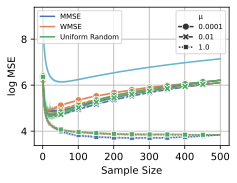
\includegraphics[width=\columnwidth]{figures/proj1/plots/GLR_MSE/BA_3_500_bandwidth_50_SNRdbs_-10.0_samps_500_mus_0.0001_0.01_1_full_band.png}
    \caption{SNR = $10^{-1}$}
    \label{GLR_BA_MSE_subfiga}
    \end{subfigure}\hfill
    \begin{subfigure}{0.3\columnwidth}
    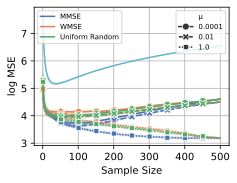
\includegraphics[width=\columnwidth]{figures/proj1/plots/GLR_MSE/BA_3_500_bandwidth_50_SNRdbs_-3.01_samps_500_mus_0.0001_0.01_1_full_band.png}
    \caption{SNR = $\frac{1}{2}$}%
    \label{GLR_BA_MSE_subfigb}%
    \end{subfigure}\hfill%
    \begin{subfigure}{0.3\columnwidth}
    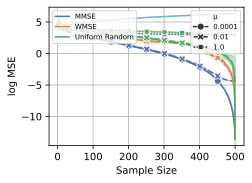
\includegraphics[width=\columnwidth]{figures/proj1/plots/GLR_MSE/BA_3_500_bandwidth_50_SNRdbs_100.0_samps_500_mus_0.0001_0.01_1_full_band.png}
    \caption{SNR = $10^{10}$}%
    \label{GLR_BA_MSE_subfigc}%
    \end{subfigure}%
    \caption{\color{black}Average MSE for GLR reconstruction on BA Graphs (\#vertices=500, bandwidth = 50) with different SNRs, line without markers is an upper bound}
\label{GLR_BA_MSE_fig}
\end{figure*}

\begin{figure*}%
    \centering
    \begin{subfigure}{0.3\columnwidth}
    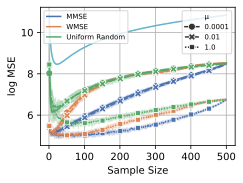
\includegraphics[width=\columnwidth]{figures/proj1/plots/GLR_MSE/BA_3_500_bandwidth_50_SNRdbs_-20.0_samps_500_mus_0.0001_0.01_1_bl_noise.png}
    \caption{SNR = $10^{-2}$}
    \label{bandlimited_GLR_BA_MSE_subfiga}
    \end{subfigure}\hfill
    \begin{subfigure}{0.3\columnwidth}
    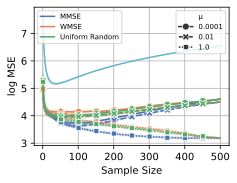
\includegraphics[width=\columnwidth]{figures/proj1/plots/GLR_MSE/BA_3_500_bandwidth_50_SNRdbs_-3.01_samps_500_mus_0.0001_0.01_1_full_band.png}
    \caption{SNR = $\frac{1}{2}$}%
    \label{bandlimited_GLR_BA_MSE_subfigb}%
    \end{subfigure}\hfill%
    \begin{subfigure}{0.3\columnwidth}
    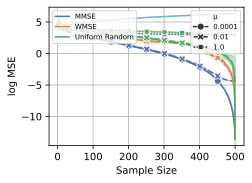
\includegraphics[width=\columnwidth]{figures/proj1/plots/GLR_MSE/BA_3_500_bandwidth_50_SNRdbs_100.0_samps_500_mus_0.0001_0.01_1_full_band.png}
    \caption{SNR = $10^{10}$}%
    \label{bandlimited_GLR_BA_MSE_subfigc}%
    \end{subfigure}%
    \caption{\color{black}Average MSE for GLR reconstruction on BA Graphs under bandlimited noise (\#vertices=500, bandwidth = 50) with different SNRs, line without markers is an upper bound}
\label{bandlimited_GLR_BA_MSE_fig}
\end{figure*}



%%%%%%%
% SBM MSE
%%%%%%%

\begin{figure*}%
    \centering
    \begin{subfigure}{0.3\columnwidth}
    \includegraphics[width=\columnwidth]{figures/proj1/plots/LS_MSE/SBM_500_bandwidth_50_SNRdbs_-10.0_samps_100_MSE_LS.png}
    \caption{SNR = $10^{-1}$}
    \label{SBM_MSE_subfiga}
    \end{subfigure}\hfill
    \begin{subfigure}{0.3\columnwidth}
    \includegraphics[width=\columnwidth]{figures/proj1/plots/LS_MSE/SBM_500_bandwidth_50_SNRdbs_20.0_samps_100_MSE_LS.png}%
    \caption{SNR = $10^{2}$}%
    \label{SBM_MSE_subfigb}%
    \end{subfigure}\hfill%
    \begin{subfigure}{0.3\columnwidth}
    \includegraphics[width=\columnwidth]{figures/proj1/plots/LS_MSE/SBM_500_bandwidth_50_SNRdbs_100.0_samps_100_MSE_LS.png}%
    \caption{SNR = $10^{10}$}%
    \label{SBM_MSE_subfigc}%
    \end{subfigure}%
    \caption{Average MSE for LS reconstruction on SBM Graphs (\#vertices=500, bandwidth = 50) with different SNRs}
\label{LS_SBM_MSE_fig}
\end{figure*}

\begin{figure*}%
    \centering
    \begin{subfigure}{0.3\columnwidth}
    \includegraphics[width=\columnwidth]{figures/proj1/LS_MSE_bl_old/SBM_500_bandwidth_50_SNRdbs_-10.0_samps_100_MSE_LS.png}
    \caption{SNR = $10^{-1}$}
    \label{bandlimited_SBM_MSE_subfiga}
    \end{subfigure}\hfill
    \begin{subfigure}{0.3\columnwidth}
    \includegraphics[width=\columnwidth]{figures/proj1/plots/LS_MSE/SBM_500_bandwidth_50_SNRdbs_0.0_samps_100_bl_MSE_LS.png}
    \caption{SNR = $1$}%
    \label{bandlimited_SBM_MSE_subfigb}%
    \end{subfigure}\hfill%
    \begin{subfigure}{0.3\columnwidth}
    \includegraphics[width=\columnwidth]{figures/proj1/LS_MSE_bl_old/SBM_500_bandwidth_50_SNRdbs_100.0_samps_100_MSE_LS.png}
    \caption{SNR = $10^{10}$}%
    \label{bandlimited_SBM_MSE_subfigc}%
    \end{subfigure}%
    \caption{\color{black}Average MSE for LS reconstruction on SBM Graphs with bandlimited noise (\#vertices=500, bandwidth = 50) with different SNRs}
\label{LS_SBM_MSE_bandlimited_fig}
\end{figure*}

\begin{figure*}%
    \centering
    \begin{subfigure}{0.3\columnwidth}
    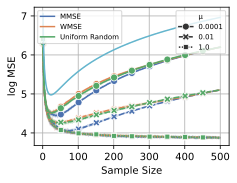
\includegraphics[width=\columnwidth]{figures/proj1/plots/GLR_MSE/SBM_500_bandwidth_50_SNRdbs_-10.0_samps_500_mus_0.0001_0.01_1_full_band.png}
    \caption{SNR = $10^{-1}$}
    \label{GLR_SBM_MSE_subfiga}
    \end{subfigure}\hfill
    \begin{subfigure}{0.3\columnwidth}
    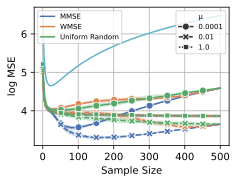
\includegraphics[width=\columnwidth]{figures/proj1/plots/GLR_MSE/SBM_500_bandwidth_50_SNRdbs_-3.01_samps_500_mus_0.0001_0.01_1_full_band.png}
    \caption{SNR = $\frac{1}{2}$}%
    \label{GLR_SBM_MSE_subfigb}%
    \end{subfigure}\hfill%
    \begin{subfigure}{0.3\columnwidth}
    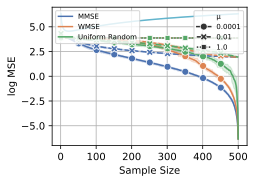
\includegraphics[width=\columnwidth]{figures/proj1/plots/GLR_MSE/SBM_500_bandwidth_50_SNRdbs_100.0_samps_500_mus_0.0001_0.01_1_full_band.png}
    \caption{SNR = $10^{10}$}%
    \label{GLR_SBM_MSE_subfigc}%
    \end{subfigure}%
    \caption{\color{black}Average MSE for GLR reconstruction on SBM Graphs (\#vertices=500, bandwidth = 50) with different SNRs, line without markers is an upper bound}
\label{GLR_SBM_MSE_fig}
\end{figure*}

\begin{figure*}%
    \centering
    \begin{subfigure}{0.3\columnwidth}
    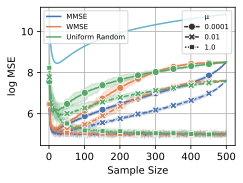
\includegraphics[width=\columnwidth]{figures/proj1/plots/GLR_MSE/SBM_500_bandwidth_50_SNRdbs_-20.0_samps_500_mus_0.0001_0.01_1_bl_noise.png}
    \caption{SNR = $10^{-2}$}
    \label{bandlimited_GLR_SBM_MSE_subfiga}
    \end{subfigure}\hfill
    \begin{subfigure}{0.3\columnwidth}
    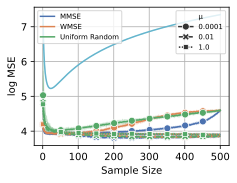
\includegraphics[width=\columnwidth]{figures/proj1/plots/GLR_MSE/SBM_500_bandwidth_50_SNRdbs_-3.01_samps_500_mus_0.0001_0.01_1_bl_noise.png}
    \caption{SNR = $\frac{1}{2}$}%
    \label{bandlimited_GLR_SBM_MSE_subfigb}%
    \end{subfigure}\hfill%
    \begin{subfigure}{0.3\columnwidth}
    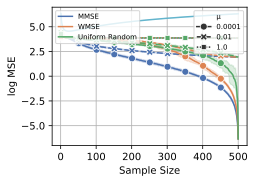
\includegraphics[width=\columnwidth]{figures/proj1/plots/GLR_MSE/SBM_500_bandwidth_50_SNRdbs_100.0_samps_500_mus_0.0001_0.01_1_bl_noise.png}
    \caption{SNR = $10^{10}$}%
    \label{bandlimited_GLR_SBM_MSE_subfigc}%
    \end{subfigure}%
    \caption{\color{black}Average MSE for GLR reconstruction on SBM Graphs under bandlimited noise (\#vertices=500, bandwidth = 50) with different SNRs, line without markers is an upper bound}
\label{bandlimited_GLR_SBM_MSE_fig}
\end{figure*}




